% ===========================
%     PREAMBLE
% ===========================

\documentclass{amsart}

% ==============================
% PACKAGES
%
% Add your own packages here
% ==============================

\usepackage{amsfonts}
\usepackage{mathrsfs}
\usepackage{amssymb}
\usepackage{amsthm}
\usepackage{amsmath}
\usepackage{mathdots}

\usepackage[all]{xy}

\def\orn{\xymatrix@C=2mm@R=4mm{
&S\ar@{}[d]|{\textcolor{red}{\Lambda_0^2}}
% \ar@/_1.5pc/[ddl]_p
\ar@/^.5pc/[ddr]
\ar@/_1pc/[dd]|(.7)\hole
% \ar[d]^k
& \\
&T^3A\ar[dl]\ar[d]\ar[dr]&\\
T^2 A & T^2A & T^2A
}}
\def\horn{\xymatrix@C=2mm@R=4mm{
&S\ar@{}[d]|{\textcolor{red}{\Lambda_1^2}}
\ar@/_.5pc/[ddl]
\ar@/^.5pc/[ddr]
& \\
&T^3A\ar[dl]\ar[d]\ar[dr]&\\
T^2 A & T^2A & T^2A
}}
\def\hhorn{\xymatrix@C=2mm@R=4mm{
&S\ar@{}[d]|{\textcolor{red}{\Lambda_2^2}}
\ar@/_.5pc/[ddl]%_p
\ar@/_1pc/[dd]|(.7)\hole
& \\
&T^3A\ar[dl]\ar[d]\ar[dr]&\\
T^2 A & T^2A & T^2A
}}

\def\cond{\xymatrix@C=4mm@R=4mm{
S \ar@{.>}[dr]\ar@/_.5pc/[ddr]\ar@/^.5pc/[drr]&& \\
& T^3 A \ar[r]^{T^2e}\ar[d]_{\mu T}& T^2 A \ar[d]\\
& T^2 A\ar[r] & ?
}}


\def\cccond{\xymatrix@C=4mm@R=4mm{
S \ar@{.>}[dr]\ar@/_.5pc/[ddr]\ar@/^.5pc/[drr]&& \\
& T^3 A \ar[r]^{T\mu}\ar[d]_{\mu T}& T^2 A \ar[d]^{\mu}\\
& T^2 A\ar[r]_{\mu} & TA
}}


\usepackage{caption}
\usepackage[inline]{enumitem}
\setlist{itemsep=0em, topsep=0em, parsep=0em}
\setlist[enumerate]{label=(\alph*)}
\usepackage{etoolbox}
\usepackage{stmaryrd}
\usepackage[dvipsnames]{xcolor}
\usepackage[]{hyperref}
\hypersetup{
  colorlinks,
  linkcolor=blue,
  citecolor=blue,
  urlcolor=blue}
\usepackage{graphicx}
\graphicspath{{assets/}}
\usepackage{mathtools}
\usepackage{mathdots}

\usepackage{tikz}
\usetikzlibrary{
  cd,
  math,
  decorations.markings,
  decorations.pathreplacing,
  positioning,
  arrows.meta,
  circuits.logic.US,
  shapes,
  calc,
  fit,
  trees,
  quotes}

\setcounter{tocdepth}{1} % Sets depth for table of contents.

% ======================================
% STYLING
%
% For those papers that need tikz (etc.) styles included
%
% ======================================


\input{./assets/paper1.tikzstyles}
\usetikzlibrary{decorations.pathmorphing}
\usetikzlibrary{decorations.markings}
\usetikzlibrary{decorations.pathreplacing}
\usetikzlibrary{arrows}
\usetikzlibrary{shapes.geometric}

\pgfdeclarelayer{edgelayer}
\pgfdeclarelayer{nodelayer}
\pgfsetlayers{edgelayer,nodelayer,main}
\tikzstyle{none}=[inner sep=0pt]


% ======================================
% MACROS
%
% Add your own macros below here
% ======================================

% Use \iam for your primary reading response
\newcommand{\iam}[1]{
  \vspace{0.25em}
  \hrule
  \vspace{0.25em}
  \textbf{{#1}'s Reading Response}
  \vspace{0.25em}
  \hrule
  \vspace{1em}
}

% Use \respond to respond to someone's primary response
\newcommand{\respond}[1]{
  \vspace{1em} \textbf{#1}
}


% Draw an (in-line) drawing of the node, given by its tikz style
% e.g. ` \node{P1X}{X} ` draws a node with style given by P1X in ./assets/paper1.tikzstyle, and labelled by `X`
\newcommand{\node}[2]{
  \begin{tikzpicture}[scale=0.3,
    every node/.style={scale=0.75}]
  \begin{pgfonlayer}{nodelayer}
    \node [style=#1] (1)   at (0, 0)   {#2};
    \node [style=none] (2)   at (-1, 0)   {};
    \node [style=none] (3)   at (1, 0)   {};
  \end{pgfonlayer}
  \begin{pgfonlayer}{edgelayer}
    \draw [-] (1.center) to (2.center);
    \draw [-] (1.center) to (3.center);
  \end{pgfonlayer}
  \end{tikzpicture}
}

  \tikzset{
     oriented WD/.style={%everything after equals replaces "oriented WD" in key.
        every to/.style={out=0,in=180,draw},
        label/.style={
           font=\everymath\expandafter{\the\everymath\scriptstyle},
           inner sep=0pt,
           node distance=2pt and -2pt},
        semithick,
        node distance=1 and 1,
        decoration={markings, mark=at position \stringdecpos with \stringdec},
        ar/.style={postaction={decorate}},
        execute at begin picture={\tikzset{
           x=\bbx, y=\bby,
           every fit/.style={inner xsep=\bbx, inner ysep=\bby}}}
        },
     string decoration/.store in=\stringdec,
     string decoration={\arrow{stealth};},
     string decoration pos/.store in=\stringdecpos,
     string decoration pos=.7,
     bbx/.store in=\bbx,
     bbx = 1.5cm,
     bby/.store in=\bby,
     bby = 1.5ex,
     bb port sep/.store in=\bbportsep,
     bb port sep=1.5,
     % bb wire sep/.store in=\bbwiresep,
     % bb wire sep=1.75ex,
     bb port length/.store in=\bbportlen,
     bb port length=4pt,
     bb penetrate/.store in=\bbpenetrate,
     bb penetrate=0,
     bb min width/.store in=\bbminwidth,
     bb min width=1cm,
     bb rounded corners/.store in=\bbcorners,
     bb rounded corners=2pt,
     bb small/.style={bb port sep=1, bb port length=2.5pt, bbx=.4cm, bb min width=.4cm,
bby=.7ex},
     bb medium/.style={bb port sep=1, bb port length=2.5pt, bbx=.4cm, bb min width=.4cm,
bby=.9ex},
     bb/.code 2 args={%When you see this key, run the code below:
        \pgfmathsetlengthmacro{\bbheight}{\bbportsep * (max(#1,#2)+1) * \bby}
        \pgfkeysalso{draw,minimum height=\bbheight,minimum width=\bbminwidth,outer
sep=0pt,
           rounded corners=\bbcorners,thick,
           prefix after command={\pgfextra{\let\fixname\tikzlastnode}},
           append after command={\pgfextra{\draw
              \ifnum #1=0{} \else foreach \i in {1,...,#1} {
                 ($(\fixname.north west)!{\i/(#1+1)}!(\fixname.south west)$) +(-
\bbportlen,0)
  coordinate (\fixname_in\i) -- +(\bbpenetrate,0) coordinate (\fixname_in\i')}\fi
  %Define the endpoints of tickmarks
              \ifnum #2=0{} \else foreach \i in {1,...,#2} {
                 ($(\fixname.north east)!{\i/(#2+1)}!(\fixname.south east)$) +(-
\bbpenetrate,0)
  coordinate (\fixname_out\i') -- +(\bbportlen,0) coordinate (\fixname_out\i)}\fi;
           }}}
     },
     bb name/.style={append after command={\pgfextra{\node[anchor=north] at
(\fixname.north) {#1};}}}
  }


% Include a tikz figure, found in the ./assets/ folder
% e.g. ` \tikzfig{paper1-CNOT} ` includes the file `./assets/paper1-CNOT.tikz`
% This makes life a lot easier if you need to move folders around.
\newcommand{\tikzfig}[1]{
\InputIfFileExists{#1}{}{\input{./assets/#1.tikz}}
}


% Refer to composition with the command \comp
\newcommand{\comp}{\circ}
% Refer to tensor product with the command \tensor
\newcommand{\tensor}{\otimes}

% bra-kets for quantum computing
\newcommand\bra[1]{\left< \, #1\, \right|}
\newcommand\ket[1]{\left|\, #1 \, \right>}
\newcommand\braket[2]{\left<\, #1 \,|\, #2 \,\right>}

%Shorthand for the set of natural numbers
\newcommand{\N}{\mathbb N}

\DeclareMathAlphabet{\mathpzc}{OT1}{pzc}{m}{it}

% ======================================
% FRONT MATTER
% ======================================

\author{ACT2019 School}
\title{Reading Responses}
\begin{document}
\maketitle{}

\tableofcontents
% ======================================
% RESPONSES FOR PAPER 0
% Example Reading Response
% ======================================

\section{Example Reading Response}
\label{sec:ex-response}

\iam{Daniel}

This is an example of how to enter your response. The
content of your response can include anything relevant to
the paper.  Some prompts are
\begin{itemize}
\item thoughts and ideas
\item worked examples
\item what you liked or disliked
\item questions about things you didn't understand
\item questions and thoughts about extentions of the paper.
\end{itemize}
But really feel free to be as creative and out of the box,
as long winded or short winded as you like.  Make
connections to other topics.

Note how I used the \verb|\iam{}| macro to introduce my primary
reading response and see how it appears on the compiled pdf.
If you have any favorite macros, feel free to include them
in the preamble. To keep this document tidy, please place
them in the MACRO's section of the preamble.  If you would
like to include any packages, you can do that in the
``packages'' sections of the preamble.

\respond{Jules} This forum is also for starting
conversations, not just giving one-off responses.  So if
you'd like to respond to someone else, you can use the
\verb|\respond{}| macro for this. Do this to answer
questions posed, ask follow-up questions, react to ideas, or
to respond with anything relevant.

You can also support your claims by citing papers. Write
the bibliography entry at the bottom of the LaTeX file. Cite
it using the command
\begin{verbatim}
    \cite{ENTRY}
\end{verbatim}
where ENTRY is what you named your reference.  Use any
format you like, this forum is an internal document only to
be seen by school participants. If the paper is available
online, link to it for convenience. Note the entry
\verb|\bibitem{CatSem}| in bibilography which, when called,
appears as \cite{CatSem}.

Quick question: what if I want to include an image into a
response?

\respond{Daniel} Even though I'm the original poster, I'm
responding to Jules, so I'll use the \verb|\respond{}|
macro.

To include images, place the file in the \verb|\assets\|
directory then by typing
\begin{verbatim}
   \begin{center}
     \includegraphics[scale=s]{FILE-NAME.XXX}
   \end{center}
\end{verbatim}
where $ 0< s \leq 1 $, FILE-NAME the name of your file, and XXX is the
extension. For example, note the file \verb|groth.jpg| in
the \verb|\assets\| directory. By including it as stated, you will see
\begin{center}
  \includegraphics[scale=0.25]{groth.jpg}
\end{center}
in the compiled document.

% ================================================
% RESPONSES FOR PAPER 1:
% ================================================

\section{A Finite Presentation of CNOT-Dihedral Operators}
\label{sec:finite-pres}


\respond{Jules}

Since you are definitely being dropped in the deep end with this paper, here's some hints to get started. Quantum computing is, to a first approximation, the study of linear maps between finite dimensional complex Hilbert spaces. Although it doesn't say explicitly, this paper lives in the symmetric monoidal groupoid [finite dimensional Hilbert spaces, unitary linear maps]. A symmetric monoidal groupoid is a symmetric monoidal category where every morphism is an isomorphism - every unitary map is invertible, where the inverse is the adjoint. (If you're rusty on linear algebra, now is a good time to get up to speed!) Every string in a string diagram represents a copy of $\mathbb C^2$, which is the state space of a qubit. So the string diagrams generate a sub-SMG whose objects are tensor powers of $\mathbb C^2$ and whose morphisms are generated by those with the matrices given in the paper.

To some extent you can think of $\mathbb C^2$ as the free Hilbert space on the set $\mathbb B = \{ 0, 1 \}$ of classical bits. The resulting basis $\{ \left| 0 \right>, \left| 1 \right> \}$ is called the `computational basis' or `Z-basis'. (That's the `Z' in `ZX calculus'.) For example, consider the classical controlled not function $CNOT : \mathbb B^2 \to \mathbb B^2$ given by $CNOT (0, b) = (0, b)$ and $CNOT (1, b) = (1, \neg b)$. (That's a function that's interesting in classical boolean circuit theory.) The linear map generated by doing $CNOT$ on the Z-basis is the quantum $CNOT$ gate. (That's definition 3.5 in the paper.) On the other hand, $T$ is a quantum gate that doesn't correspond to anything in classical circuit theory.

\respond{Hector}
For people new to diagrammatic calculi:

\begin{itemize}
\item Rather than express everything using a single line of maps joined by $\comp$ and $\tensor$,
for example $ (f \tensor id ) \comp (id \tensor g)$,
we express that same information by a diagram, where $\tensor$ is shown by maps placed side-by-side,
and $\comp$ shown by maps placed one-after-the-other and joined by a wire.
You can see the equation $ (f \tensor id ) \comp (id \tensor g) = (id \tensor g) \comp (f \tensor id ) $
written out as a diagram in \S 2.

\item Every circuit diagram can be rewritten back in usual $\tensor$ and $\comp$ form,
and every morphism built from $\comp$ and $\tensor$ can be written as a diagram.
It becomes really useful to use diagrams when dealing with complicated systems,
especially because it makes rules like those in \S 2 easy to see.

\item This paper's diagrams are read left-to-right (as is conventional for circuit diagrams.)
This means that wires should always be going left-to-right (signifying $\comp$)
and $\tensor$ is shown by subdiagrams being placed one above the other.

\item $n$ wires stacked on top of each other means $n$ $\tensor$-copies of $\mathbb{C}^2$. A bare wire signifies the identity.
The letter $I$ as an object is reserved for the monoidal unit, which in this category is $\mathbb{C}$,
but the letter $I$ as a morphism refers to the identity.

\item For example: Definition 3.1 defines the gate $X$ which sends one input (on the left) to one output (on the right.)
$X$ acts as as a matrix $X: \mathbb C^2 \to \mathbb C^2$.

\item \emph{Gate} means a morphism that has the same number of inputs as outputs.

\item Defintion 3.2 defines the gate $U$ (sending two wires on the left to two wires on the right) in terms of earlier gates.
That diagrammatic definition is equivalent to writing $U := CNOT \comp ( I \tensor X) \comp CNOT$.
If we were to express $U$ as a matrix it act as $U: (\mathbb C^2)^{\tensor 2} \to (\mathbb C^2)^{\tensor 2}$,
and we could work out its matrix form by the usual $\comp$ and $\tensor$ of the $X$, $I$ and $CNOT$ matrices.

\item $CNOT$ is drawn that way because of things Jules mentioned:
That $CNOT$ works like the identity on the first entry,
but on the second entry it acts like either $I$ or $X$
depending on whether the value of the first entry was $\ket{0}$ or $\ket{1}$.
We say that the first entry (the top wire) controls the second entry (the bottom wire.)
We will see something similar in the paper 2.
\end{itemize}

Here are some macros for displaying certain nodes (or just write diagrams out with $\tensor$ and $\comp$,)
and for anyone who wants to use tikz diagrams I have put together the file ./assets/paper1.tikzstyle.
\begin{align*}
\text{Gate} & \quad \text{Diagram} \\
X & \quad \node{P1X}{X} \\
T & \quad  \node{P1T}{T} \\
CNOT & \quad  \tikzfig{paper1-CNOT}
\\
U & \quad  \tikzfig{paper1-U}
\\
V & \quad \tikzfig{paper1-V}
\\
\end{align*}

\respond{Brendan}
Another option for drawing string diagrams is the proto-TikZ package David
Spivak and I use. It can be found here:
\url{https://github.com/appliedcategorytheory/TikZWD}. It was largely
developed by Patrick Schultz, so credit to him. Please feel free to use,
redevelop, and to push improvements to the repo!

\[
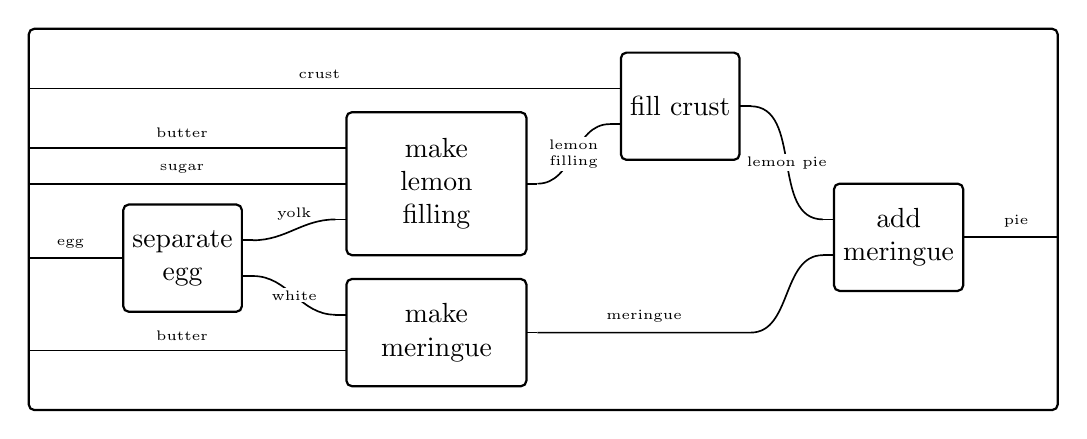
\begin{tikzpicture}[oriented WD, align=center, bbx=1.2cm, bby=2ex]
  \node[bb={3}{1}, bb min width=.9in] (filling) {make\\lemon\\filling};
  \node[bb={2}{1}, bb min width=.9in, below=of filling] (meringue) {make\\meringue};
  \node at ($(filling.west)!.5!(meringue.west)$) (helper) {};
  \node[bb={1}{2}, left = of helper] (separate) {separate\\egg};
  \node[bb={2}{1}, above right = -2 and 1 of filling] (fill) {fill crust};
  \node[bb={2}{1}, below right = of fill] (finish) {add\\meringue};
  \node[bb={0}{0}, fit=(separate) (meringue) (fill) (finish)] (pie) {};
%
\begin{scope}[font=\tiny]
  \draw (pie.west|-fill_in1) to node[above] {crust} (fill_in1);
  \draw (pie.west|-filling_in1) to node[above] {butter} (filling_in1);
  \draw (pie.west|-filling_in2) to node[above] {sugar} (filling_in2);
  \draw (pie.west|-separate_in1) to node[above] {egg} (separate_in1);
  \draw (pie.west|-meringue_in2) to node[above] {butter} (meringue_in2);
  \draw (separate_out1) to node[above] {yolk} (filling_in3);
  \draw (separate_out2) to node[fill=white, inner sep=0.8pt] {white} (meringue_in1);
  \draw (filling_out1) to node[fill=white, inner sep=0.8pt] {lemon\\filling} (fill_in2);
  \draw (fill_out1) to node[fill=white, inner sep=0.8pt] {lemon pie} (finish_in1);
  \draw let \p1=(fill.east|-meringue_out1), \n1=\bbportlen in
    (meringue_out1) to node[above] {meringue} (\x1+\n1,\y1) to (finish_in2);
  \draw (finish_out1) to node[above] {pie} (finish_out1-|pie.east);
\end{scope}
\end{tikzpicture}
\]


\iam{Mario}
This is probably a recurrent theme in all branches of applied category
theory, but I think the graphical calculus (e.g.\ having ladders, stairs\ldots)
here made following the general idea of the proof much more intuitive.

The paper proves the existence of a normal form for each CNOT-dihedral
operator but it does not give an algorithm to compute it. On its
conclusion it says the following.
\begin{quotation}
  This is because the proof of Proposition 5.5 appeals
  non-constructively to properties of the ambient symmetric monoidal
  structure.
\end{quotation}
I tried to track down this source of
\textit{non-constructiveness}, but I am a
bit confused. Coherence is used in Lemma 5.1, but only to say that a
SWAP gate can be expressed as a sequence of two-bit swap gates, so I
guess this is not problematic (is it?).  The proof of existence of a normal
form for diagonal circuits in Lemma 5.3 looks like an algorithm; and
Lafont in~\cite{LafontBooleanCircuits} seems to describe a
(canonical?) rewriting system.  Where exactly do we encounter
problems if we try to implement Lemma 5.5?

I also started trying to read~\cite{RewritingSMC}. There, it seems
that only the connectivity of the diagrams is considered, taking them
to be hypergraphs.  The paper mentions that the techniques there could
be used for CNOT-dihedral circuits.  This is probably obvious but I am
not sure if I am missing something: considering we start from a
circuit, will there be a canonical way of getting back a
\textit{circuit} after the transformations?

\respond{Fatimah}
I also thought about this, and the way I convinced myself is that relations of page 92 show us the commutation relation between each pair of operators, and to prove 5.5 they use the fact that we have these relations! But it is non-constructive because if I give you a circuit with 1000 gates, given this theorem you are sure, you can find a normal form, but this theorem does not tell you, how you can get the normal form, for example, should I start from middle gates or should I move diagonal gates first and next affine gates or vice versa and so on!
But maybe I am wrong!

\respond{Hector}
``will there be a canonical way of getting back a
\textit{circuit} after the transformations?'' -- this is referred to as \emph{circuit extraction},
and is very much an active topic in the field.
Recent results (e.g. \cite{Duncan19})
focus on how to perform optimisation strategies while preserving
certain properties that will guarantee a circuit extraction at the end.

I believe the non-constructiveness of Lemma 5.5 comes from Theorem 11 of \cite{LafontBooleanCircuits},
where the terms of Figure 18 do not give a terminating rewrite strategy.

As such you know this normal form exists, but not how to get to it.
If you are given the map $U = \omega^{p_(x_1, \dots, x_n)}\ket{q(x_1, \dots, x_n)}$
and tasked to write down a circuit that performs $U$ then you can use this normal form to do so.
Given a circuit and asked to work out a map of the form $U$ that describes the action of the circuit is a far harder task
(I suspect someone with knowledge of complexity theory can weigh in and tell us how hard.)

\respond{Mario}

Thank you both! I think I see this now. If anyone is interested, as
Hector says, in Theorem 11 of~\cite{LafontBooleanCircuits} Lafont
mentions that ``the existence of a terminating rewrite system for
$GL(Z_2)$ is an open question.''.  Thank you also for the pointer to
the circuit extraction paper.

\iam{Sophie}

To keep my head on straight, I wanted to draw some parallels with group presentations:
\begin{itemize}
    \item CNOT-dihedral operators are elements form a symmetric monoidal groupoid, the same way the set of rotations and flips of a square form a group (namely the dihedral group $D_4$). The group $D_4$ has generators (rotations and flips) and relations ($r^4 = f^2 = 1, rf = fr^3$). The symmetric monoidal groupoid similarly has a set of generators and relations. The generators (and derived generators) are divided into two types: diagonal and affine. The diagonal ones ``scale" the bits and  the affine ones are a more interdependent  linear combination of the bits. In Remark 3.8, it is said that the relations are not known to be minimal (although they are independent) meaning it's possible that there is a set of fewer relations which generate the relations given here. I've been trying to come up with a group presentation with independent but not minimal relations and haven't found anything interesting.
    \item Every operator has a unique normal form. This is like in the group $\mathbb Z^2 = \left< a, b | ab = ba\right>$ we have $abbbba = abbabb = ababbb$ so there are lots of ways of writing the same element. But we can say that the normal form of an element is the form in which all of the $a$s are written before all of the $b$s. So the normal form of the above is $aabbbb$. By applying the relations there is exactly one way to write each element in normal form. In the group setting the normal form makes it easy to read off some information about the element. For example, the normal form given above makes it easy to read off how many $a$s and how many $b$s there are. Are there any useful properties that can be read off of the operator normal form?

    \item Where does the choice of the operator normal form come from? Does it reflect some intuitions from quantum computation? It seems possible that different normal forms are more useful depending on what questions you are asking. For example, what if instead of wondering how many $a$s and how many $b$s there are, I just want to know if there are more $a$s or $b$s? Then I might choose the normal form ``interleave $a$s and $b$s and then put whatever is remaining at the end" so the new normal form of $aabbbb$ would be $ababbb$. Now, to determine if there are more $a$s or $b$s you just have to look at the last two characters. How easy!
\end{itemize}


\respond{Brandon}

A simple example of a group with independent non-minimal relations is
$$\langle x | x^4, x^6 \rangle$$
where the two relations are independent but are equivalent to
$$\langle x | x^2 \rangle$$
but this one is probably not very interesting.

In a perhaps more interesting example, the ``even subgroup'' of the free group of rank 2 (on $x,y$) containing even length words is generated by $\langle x^2, y^2, xy, yx \rangle$ where these generators are independent (I'm pretty sure) but not minimal as $\langle x^2, xy, xy^{-1} \rangle$ generate the same group.  So in the quotient by this subgroup we have presentations
$$\langle x,y | x^2, y^2, xy, yx \rangle = \langle x,y | x^2, xy, xy^{-1} \rangle$$
but I guess this is just another pair of presentations of $\mathbb{Z}/2$.


\iam{Dan}

I am relatively new to Quantum computing, so the aspect of this paper that most stood out to me was how similar the proofs felt to traditional linear algebra proofs. The ``decomposition'' of an arbitrary CNOT-dihedral circuit into the product of a diagonal normal form circuit $D'$ and an affine normal form circuit $A'$ is highly reminiscent of elementary matrix algorithms like the QR factorization or the SVD. I suppose this isn't too surprising, given Jules' comment on the relationship between quantum circuits and linear maps between finite dimensional complex Hilbert spaces. This does make me wonder to what degree these connections might be more clear if we used more familar notation. While the circuit diagrams do make it easier to see relationships between different complicated circuits, the additonal abstraction they apply can obfuscate the actual operations that the circuits perform.

One other area of confusion for me is the properties of the normal form for CNOT-dihedral circuit. The authors demonstrate that normal forms always exist and are unique. However, it's not clear to me whether the authors' normal form is the only structured form with these properties. If this is not the case, it's unclear what is ``special'' about the $D'A'$ presentation other than its uniqueness and existence.

Also, like some of the other students I was confused by the assertion that Proposition 5.5 is inherently non-constructive and does not contain an algorithm to compute the normal form of an arbirary CNOT-dihedral circuit. My understanding is that Proposition 5.5 defines the following pseudo-algorithm:
\\
\textit{Input}: A CNOT-dihedral circuit $C$\\
\textit{Output}: The normal form of C, $D'A'$\\
\begin{enumerate}
    \item Write $C$ as the product $DA$, where $D$ is a diagonal circuit and $A$ is an affine circuit (Described as an algorithm in the proof of Lemma 5.1)
    \item Convert $D$ to diagonal normal form $D'$ (Described as an algorithm in the proof of Lemma 5.3)
    \item Convert $A$ to affine normal form $A'$ (Proven possible in \cite{LafontBooleanCircuits}, but only a pseudo-algorithm is described in Theorum 11)
\end{enumerate}

\iam{John}

It is quite interesting to view this paper trough the lens of the ZX-calculus (which will be the topic of next week). The gates $U$ and $V$ defined in this paper have a nice representation in the ZX-calculus in terms of \emph{phase-gadgets} (and in fact, such gates also correspond to the commonly used Molmer-Sorensen gates in ion trap quantum computing, and the two-qubit gate of superconducting quantum computing). Using this representation in the ZX-calculus, all the rewrite rules, except for $R_{13}$ are quite easy to prove. In fact, as far as I know, there still is no direct proof of this equality in the ZX-calculus.

Like other people, I am a bit confused that the paper remarks that this paper does not give a algorithm for computing the normal form. The part where they separate the diagonal and the affine portion is definitely constructive, and the forming of the normal form of the diagonal part is also constructive, so there must be a problem in reducing the affine portion to the normal form. I think this might be because it involves some combination of SWAP and CNOTs gate where it is not clear how many SWAPs there should be.


\iam{Brandon}

This paper felt pretty approachable even given my irrational fear of complex linear algebra.  I liked the intro to the graphical language, which makes diagrams in a symmetric monoidal category much easier to read and think about (I'm new to string diagram type things but a big fan so far).  I know that this is moreover a groupoid, though I'm not sure I saw how that was reflected in the graphical techniques: was there anything in there that couldn't have worked just as well without operators being invertible?
\respond{Fatimah}
I think because they are quantum gates, and quantum gates should be unitary.

The general structure of the paper was a process familiar from group theory of describing a group via generators and relations, and giving a normal form of words in those generators uniquely determining each element in the group.  Sophie describes this in more detail above and I too am curious about the questions she asks regarding why this normal form was chosen and what properties of an operator it highlights.

I found the phase polynomials a bit tough to read through (especially with the mixing of $\mathbb{Z}/2$ and $\mathbb{Z}/8$ coefficients), but I can see how they would be efficient tools for verifying expressions in the graphical language.

I think my biggest confusion throughout this paper was about the motivation and significance of these particular operators, since I have very little background in quantum computing.  For instance, I have a hard time interpreting what the derived generators and components of the normal form really do, and I have no idea how to interpret phase shifts like $\omega$ or $T$.  I'm also not sure I see the reason for restricting to operators of order 16; is this just an approachable subproblem of a larger group, or does it have some computational significance?

\iam{Georgios}

This paper comes out of the left field for me
in the sense that it covers a lot of ground
on a field that I know nothing about (namely, quantum computing),
which is already covered by other papers in the field---understandably.
I like the use of string diagrams, even though I don't understand \emph{all}
the math present in this paper I got enough of an idea
to understand the composition of those gates.

However, because of my unfamiliarity with the subject I have
three rather ``practical'' question:
\begin{enumerate}
\item How do those gates assist with quantum fault tolerance in general?
\item For that matter of fact, how is quantum fault tolerance different
  than fault tolerance in digital systems (I get that it has to be different
  but in what way)?
\item I can see how reducing to some normal form is useful---once
  I understand how quantum fault tolerance is assured by using those gates---but
  it seems like there are other formalisms that reach similar (?)
  conclusions. If that is indeed the case, how is this formalism better?
  I am a little unsatisfied by the answer that it uses a common language---but
  that may very well be an interesting position in the event that other
  formal systems are too complicated to actually use.
\end{enumerate}

\iam{Fosco}

May of the questions I had in mind after reading the  paper have been solved by reading other people's reading responses: thank you all! The paper is evidently well-written, but I suffered from my lack of preliminaries. In particular, I am completely new to most of the aspects discussed here apart having a certain acquaintance with the rules of graphical calculus; thus, since the very beginning I felt a friendlier introduction to the rules of graphical calculus was needed. It is of course my fault, as I must admit I felt a bit lost right after the first preliminaries.

Just an example of something I feel the need to clarify in my head: after a moment of reflection, CNOT is evidently equal to $I\oplus X$, where $I$ is the identity matrix of $\mathbb C^2$. Although the monoidal structure on the groupoid $\bf Hilb$ given by coproduct $\oplus$ is never mentioned or used, in favor of the more natural choice of $\otimes$, I think this suggests that there is some additional structure on $\bf Hilb$ that can be translated into graphical calculus: $\bf Hilb$ is a \href{https://ncatlab.org/nlab/show/rig+category}{rig category}.

My question (admittedly focused on a minor detail) is then: how far can the rule that a ``vertical strand'' connecting two operators $A,B$ denotes their direct sum $A\oplus B$ be taken? Such strands appear all along the relations in Fig. 1, and not only for the CNOT gate; see e.g. $R_{13}$.

Is there a full-fledged graphical calculus for \emph{distributive monoidal} and rig categories?

\respond{Christian} That is a great observation and question. After a brief search, I did not find a graphical calculus for rig categories, which is somewhat surprising. There is Selinger's overview of many existing graphical languages \cite{SelingerSurvey}; they only mention ``going beyond a single tensor product'' toward the very end. Perhaps this has not yet been explored! We should look into this.

\respond{Alexis} I'm super interested in rig categories too! As for graphical calculi for categories with more than one monoidal products, there are two distinct approaches that I'm aware of. The first one from Girard are proof nets: they look a lot like string diagrams, but the crucial property that you lose when working with them is that not all diagrams encode valid proof nets.

Any string diagram built from composition and tensor of generators corresponds to a valid morphism in a monoidal category --- in the same way as any concatenation of monoid elements encodes a valid monoid element. Whereas for proof nets you need an additional correctness criteria --- in a similar way as for categories, where you need to check that domain and codomains match for a concatenation of morphisms to encode a valid morphism.

A second approach from Melliès, which is very related to proof nets, is that of functorial boxes. Essentially you could draw a string diagram with boxes around some of the morphisms, where concatenation of morphisms outside of the box is the tensor product, and inside of the box is the direct sum. Then the boxes encode the exponential functor sending direct sum to tensor product.

I've never really worked with either of them so I can't really tell much, but they surely are worth looking into. To go back to quantum computation, this paper \cite{AbramskyDuncan06} model protocols like teleportation and entanglement swapping using proof nets.
\\

\iam{Bruno}

As somebody with a background in Computer Science, quantum fault-tolerant
computing presents a radically different topic than the one I'm familiar with.
There seem to be a lot of technical details present in the paper, building very
intricate structures on top of already assumed foundations.

The intuitive thing that immediately clicks for me is the graphical notation; leaving out
topologically invariant details to be efficiently processed by our visual cortex
seems to be a useful aid in reasoning.

However, an obstacle to understanding the paper is the inherent complexity of the circuits. Not that I'm not claiming they are hard to understand for somebody with the sufficient background, but rather that the specification and special rules imposed seem at a first glance monolithic and non-compositional.

Some of the questions that immediately came up for me were:
\begin{itemize}
\item Why is the $\{CNOT,T, X\}$ gate focus of the recent studies of quantum circuits?
\item Why are there 4 generators for CNOT-dihedral operators?
\item How do the 4 generators give rise to the so many ``special rules''? (they
  at least seem special, as presented in paper's figures)
\item How is the presented circuit algebra different than the standard
  fault-tolerant algebra used in regular electric circuits?

\end{itemize}

\iam{Adam}
I enjoyed this paper, not least because it gave me my first opportunity in a while to revisit quantum computing  (and because the diagrams are so pretty and easy to look at!). I think I followed the main argument of the paper though it took me a little while to figure out how it all fit together, so I'll summarise what I thought the article was saying here and people can jump in to correct me if I've totally missed the point or offended anyone's sensibilities (mathematical or otherwise):
\begin{itemize}
  \item The paper gives a set of relations $\mathbf{R} = \{R_1-R_13\}$ for (graphically) rewriting quantum circuits made from the CNOT-dihedral gates $\{X, T, CNOT \}$ (and $SWAP$ (which we have for free) plus some derived gates $U$ and $V$ are added and appear in the relations to aid the argument)
  \item To show this constitutes a "presentation" for the symmetric monoidal groupoid we need to prove that any two CNOT-dihedral circuits on n-qubits defining the same operation can be transformed into each other using out relations from $\mathbf{R}$
  \item One way to prove something like this is to show that there is some normal form into which every circuit (constructed from our chosen gates) can be transformed using relations from $\mathbf{R}$ and that distinct normal forms define distinct operations.
  \item In fact, such a proof seems to be what Lafont \cite{LafontBooleanCircuits} did for circuits made from the \textit{affine} gates $\{X, CNOT, SWAP\}$ with relations $\{R_1, \dots R_6 \}$ (this wasn't clear to me until my second reading of this paper as it didn't seem clear that Lafont's paper assumed the same (or an equivalent) set of relations).
  \item Additionally the authors prove a similar result for the \textit{diagonal} gates $\{T, U, V \}$  with relations $\{R_7, \dots R_10\}$. (in lemmas 5.2 and 6.2)
  \item So, the main result of the paper follows then from showing that adding relations $R_11, R_12,$ and $R_13$ lets you rearrange any CNOT-dihedral circuits so the affine gates come after the diagonal ones (lemma 5.1) (So you get a unique normal form for CNOT-dihedral from the NFs for affine and diagonal gates)

\end{itemize}

I gather from the other posts that the I'm not alone in saying that one of the the main things that confused me in the paper was layout of the affine normal form. Can anyone shed some light on what the  motivation for/wisdom behind this is? (is this idea of "ladders" somewhat standard in QC/ACT? as it definitely didn't feel intuitive to me the first time around.)
\\
Other questions I had about this field when reading this were:
\begin{enumerate}
  \item The paper says we don't know if $\mathbf{R}$ is minimal for this CNOT-dihedral circuits. Do we know if $\{R1, \dots R_6\}$ is minimal for affine circuits? (or $\{R_7, \dots R-10\}$ for diagonal ones?)
  \item Has anyone written a program for rearranging circuit diagrams like this? It seemed like a tempting thing to do if one had more time...
\end{enumerate}

\iam{Nathan}

Like others, I am relatively new to both quantum computation, and diagrammatic languages, so this paper was a bit of a challenge to understand. I think I get the basic idea behind the graphical calculus used in the paper (which is similar to the sort of string-diagrammatic calculi I've seen before, but written in a more ''circuit-friendly'' form), but mainly had some difficulty understanding the definitions relating to the normal forms used in the paper. For instance, while I think the definition of ladders and ascending stairs is pretty clear, in definition 4.3, I'm a bit confused as to what the single boxes with an $\mathscr{X}$ are supposed to represent. Are these supposed to be just $X$ gates? And definitions 4.6 and 4.7 are even less clear to me. Thus, it was rather difficult for me to wrap my head around the rest of the paper.

I do find the approach of tying to understand quantum circuits (for arbitrary qubits $n$) by presenting a symmetric monoidal groupoid using such a generators and relations, as opposed to fixing $n$ and working with mere group presentations to be an interesting idea though. In general, I like thinking about things from a ``generators and relations'' perspective, and I would very much like to learn more about approaches to study categories themselves from that perspective, as is done in the paper, but unfortounately without the background knowledge it was difficult for me to get much out of this paper. Perhaps others will be able to help me with some of my notational confusion, and I'll be able to get more out of it on my second read-around.

\iam{Diego}

Like several other responses echo, graphical diagrams are one of the great tools that
thinking in categorical terms provides. This includes having relations to keep
the thinking completely in graphical terms.

One thing that I have personally struggled with diagrams is that often times there are
some relations that feel magical, like $R_{13}$. I'm not sure how the relations are
discovered. It feels like this is only clarified until
the effects of the gates on the phases is clarified.
In a similar sentiment, I feel that most of the work is done in a higher level than
the graphical diagrams. There is a lot of computation left to the readers that feels like either should
be formally addressed or be informally dealt with.

In a different line of thought,
the diagonal normal form seems overly complex. As I understand it, the important characteristic
of the $U$ part is that every pair of qubits has a number of $U$ gates applied. The particular
shape exists to enforce uniqueness. Similarly, the important
characteristic of the $V$ part is that every trio of qubits has a number of $V$ gates applied.
And for the sake of completeness, the important characteristic of the $T$ part is that
every qubit has a number of $T$ gates applied. Since everything commutes, composing functions
one after the other obscures what's happening, as the important thing is the multiset of these
applications. In other words, the diagonal normal form is unique but not canonical.

The current gates can't produce entangled states, mostly because they all map a base
to another one, modulo phases. I wonder what are the effects of including a set of gates
that could create entanglement in the relations needed?

\iam{Derek}

I'm also one with only a passing familiarity with the formalisms used in quantum computing. That said,
the math itself in this paper seemed mostly just motivated by quantum computing but otherwise relatively straightforward
if intricate calculations once you have the candidate for the normal form. The paper doesn't go into much
detail about how the normal form was discovered, as pointed out by others.

I'm much more comfortable with the diagrammatic reasoning and symmetric monoidal categories/groupoids as it
has connections to linear logic. I imagine the impact of an SMG as opposed to an SMC would be something like
a (classical) reversible computing framework. There's a good amount of programming language theory work on
making higher-level reversible languages. This would be a bit of a step back from the diagrammatic approach,
but it's likely some of the patterns (e.g. the $U$ triangles) as well as the relations are more intuitive at
the level of a quantum programming language. Specifically, my guess would be that the patterns would be more
like compilation artifacts, while the relations would become relatively straightforward equivalences of code
in a quantum programming language.

Peter Selinger's survey~\cite{SelingerSurvey} of diagrammatic languages for monoidal categories of various types
seems useful. Adding elaborations to the graphical language roughly like some of the ones described in this survey
may be a way to bring the high-level quantum programming language perspective back to a diagrammatic perspective, if
desired. Indeed, the triangles and ladders notation is an example of extending the graphical language, but I don't
know if it is well motivated outside the context of establishing this normal form. What do these triangles and ladders
mean at the level of (quantum) computations, in the sense that I would describe an adder circuit as performing addition
not the particular Boolean function it calculates?

\iam{Christian}

I appreciate everyone's thoughts; I was a bit lost trying to read this alone. I empathize with your responses. I am also new to this whole subject; I only vaguely know that quantum computing involves complex linear algebra. It seems like great stuff, and I decided to start reading Picturing Quantum Processes \cite{PQP}. I can see that this is a whole vibrant world of research, and I am looking forward to discussing this subject with you all into the future.

For this paper, I share the communal wondering as to the motivation. The presentation of the symmetric monoidal groupoid in terms of the basic gates T, X, CNOT is very nice, though it takes time to build intuition of how they transform qubits and why they are universal (and the meaning of the distinction between affine and diagonal). As many have said, though, the reasoning for the paper is not entirely clear. Of course, normal forms are essential for computation. But why these? How were they determined? What will be done with them? I'm sure these questions can be answered through a literature search, and consulting mentors; we will figure it out.

I am very interested in the idea of generalizing the ``presentation'' of algebraic structures from one-sorted theories, such as monoids, to multisorted theories, such as categories. The general framework exemplified here has been formalized in terms of pseudomonads \cite{Pseudomonad}; for example, there is a ``free symmetric monoidal groupoid'' pseudomonad on $\mathrm{Cat}$, one algebra of which is the CNOT-Dihedral Operator calculus. This level of generality embraces computer science and category theory under the beautiful umbrella of higher algebra, which for too long has been a secret of the upper categorical echelons. These ideas could help connect quantum computing languages with other mathematical concepts; I may look into this more.

More concretely: in the case of unitary gates, adjoints and inverses coincide - is that what makes this calculus ``circuitous'', as opposed to the ``string'' general formalism? What are the primary differences of this language from the ZX-calculus? I think I would be able to ask more intelligent questions after reading the Lafont paper, but I am already late to the party. Looking forward to the discussion tomorrow.

The gate colors are nice. I want to do research that involves graphical languages.

\iam{Bryce}

Without repeating what others have shared, I too enjoy the graphical calculus, however I wonder if it necessary.
Given that we have matrix representations for each of the generators, one could also represent the derived generators as matrices, for example \ldots
\[
  \tikzfig{paper1-U} =
    \begin{bmatrix}
        1 & 0 & 0 & 0 \\
        0 & 1 & 0 & 0 \\
        0 & 0 & \omega & 0 \\
        0 & 0 & 0 & 1
     \end{bmatrix}
\]
% Add in other matrix calculation.
\ldots if I haven't made any mistakes (perhaps someone else calculate the other one). However I am not sure if this perspective is actually useful for the rest of the paper. Does it make any of the computations easier?

\respond{Alexis} One way to see how much easier computation can get with circuit diagrams (or more generally string diagrams for tensor networks) as opposed to writing down explicit matrices is that in general the matrix form will be exponentially bigger than the diagram. Indeed, as each wire represents a copy $\mathbb{C}^2$ and their concatenation encodes the tensor product, a diagram with $n$ wires will encode a $2^n \times 2^n$ matrix.
You needed $16$ matrix entries to represent $2$ gates, so imagine writing down all of the $256$ entries corresponding to the $5$ gates of the left-hand side of $R_{13}$.
\linebreak

 Admittedly I haven't had a much time to read this week as I would like, so I will try and edit this response later with some more.


 \iam{Alexis}

 I was already quite familiar with the ZX-calculus and quantum computation with string diagrams in general, but it's very nice to read the thoughts and questions of people from different backgrounds.

 I'm especially interested by the discussion about the constructivity of the normal form, and like others I have a hard time pinpointing the exact place where non-constructivity comes in.
 Assuming that we could come up with a decision procedure for computing the normal forms, a natural question (which was mentioned above by Hector) would be: what is the computational complexity of this procedure? i.e. given a circuit with $n$ gates, can we find a bound on the number of rewrite rules needed to get to normal form?

 Considering that the size of the matrix can be exponentially bigger than that of the corresponding circuit, one would expect the problem to be at most in \textsc{Exptime} (just compute all of the matrix entries). Because we can compute these entries one at a time, reusing space, I'm guessing this should give a \textsc{Pspace} algorithm. Going down the hierarchy one step further, can we show the problem is in \textsc{NP}? This would amount to showing that there exists a proof (a certificate) with at most a polynomial number of rewrites.

\iam{Toby}

I am shamefully late to the party this week, but as a result I have enjoyed reading the responses of the more dilligent of you -- thanks! (Like many of the others, I too am not an expect in quantum computing -- so please forgive the inevitable errors in what follows.)

A couple of people above have mentioned $\bf Hilb$, the category in which we normally think of quantum circuits as living, but one of the things I liked about the presentation in the paper is that it only makes implicit reference to that ambient category -- through labels such as `affine' and `diagonal', and by having to prove lemma 5.2 that ``diagonal gates commute'' -- and instead focuses only on its particular symmetric monoidal groupoid structure. At the beginning of section 3, the authors give matrix representations of their generators, but it seems to me that their results do not depend on these particular representations, and so their results should also apply to CNOT-dihedral circuits in any other symmetric monoidal groupoid.

Now, that probably isn't particularly interesting, but like Mario, it makes me wonder about the general theory of rewriting in symmetric monoidal categories \cite{RewritingSMC}. In particular, one of the most pleasing aspects of \textit{Picturing Quantum Processes} \cite{PQP} is its extremism: its ambition seems to be to have entirely graphical proofs of results in quantum computing. By contrast, the authors in this paper frequently translate their circuits into the ``phase polynomial representation''. It seems that, at the cost of requiring explicitly that the symmetric monoidal groupoid admits sums, this representation could also have been given graphically -- though I can't say that that would have added anything to this paper apart from a pleasing aesthetic.

A number of responses above have mentioned the non-constructivity of the main result (I think I agree with Fatimah's intuition); and I am also interested in the open question about whether the given presentation is minimal. Like the others, I can't help wondering if there exists a general algorithm (with a useful complexity) for `compiling' a hypergraph circuit into a (unique?) normal form, given some set of relations. Is that the context in which we should take the work of Bonchi \textit{et al.} \cite{RewritingSMC}? I can imagine that such an algorithm could be useful also in biology: consider a complex experimentally determined gene regulatory network; understanding its `normal form' might well be pharmaceutically useful.

I did of course also have some technical questions arising from my naivety, such as ``where did those particular relations come from?'', and ``why is the $U$ gate defined that way?''. But those are less interesting to me than the general theory.

\iam{David}

I am even more shamefully late to the party than Toby, so I had the added benefit of reading their response as well as everyone else's. I also found myself a little bewildered in new territory; mostly I felt (along with Diego) that some of the relations were pure magic. How could you discover this? I suppose by playing around diligently.

I am struck again by the persistence of graphical languages in remaining intuitive against all calculational odds. In particular, I am thinking of the commutation rules in Figure 2, which (apart from the big one in the middle) are generally of the form ``slide this past that" familiar from the `Yangs-Baxter' or bifunctoriality equations. I'd hope that a good notation for direct sums could make some of these even more obvious -- and maybe if we put ``phases'' on our diagrams we could find the ones involving $\node{P1T}{T}$ to be just a matter of sliding things around.

How ``literal'' can one take these diagrams? Would a quantum circuit look like a diagram like this, the way a wiring diagram for a circuit looks like a blown up version of that circuit? Can I imaging particles travelling through the circuit, being affected by the boxes?

Now, I don't know any quantum physics. The only thing I've seen is Bob Coecke's \emph{Kindergarten Quantum Mechanics} (see URL below)
-- and I'm not sure I'm ready to graduate Kindergarten yet. On page 8, Coecke gives the quantum teleportation and proof of its correctness. At the bottom of the page, they cite a ``usual textbook approach''. This textbook approach describes Alice using a CNOT gate. The thing is, I don't see a CNOT gate happening in Coecke's string diagrams, and I'm not sure how to see one if I did.

So I think the string diagrams are the same, except that this paper has some more names which don't appear in Coecke's paper because they're not getting that specific. But because Coecke doesn't have a notation (for kindergarteners at least) for direct sum, we can't express CNOT out of smaller parts. The teleportation proof given by Coecke doesn't need it though, where the textbook one cited uses it. Could anyone help me understand the difference? Is the difference that Coecke is teleporting any finite quantum system (i.e. the string could be any finite dimensional hilbert space) whereas the textbook example specifically teleports a single qubit?


\url{https://arxiv.org/pdf/quant-ph/0510032.pdf}


\iam{Miriam}

In the Zoom meeting about this paper, participants brought up a couple of questions that I wanted to answer. Apologies for the delay in posting this.

\textit{The complexity of CNOT-dihedral circuits}: CNOT-dihedral circuits are efficiently classically simulable. I don't know why this result is not mentioned anywhere in the Amy et al.\ paper -- it does appear in one of their references, \cite{Scalablerandomised}, which is the original paper to introduce the concept of CNOT-dihedral circuits.
The efficient classical simulability of CNOT-dihedral circuits plays an important role in that paper because the authors propose to use them as a randomised benchmarking scheme. The question of complexity is specifically addressed in the paragraph ``Efficient computation in $G_{2^k}$'' \cite[p.~3]{Scalablerandomised}.

\textit{Universality of the Clifford+$T$ gate set}: The Clifford+$T$ gate set corresponds to the set of CNOT-dihedral gates together with the Hadamard gate.
As indicated in the previous paragraph, CNOT-dihedral circuits are efficiently classically simulable, but adding Hadamard gates promotes their computational power to full quantum computation. (This is analogous to the better-known case of Clifford circuits, which are classically simulable but gain the full power of quantum computation if $T$ gates are added.)
The universality of the Clifford+T gate set was originally proved in \cite{universalfaulttolerant}. Note that the paper uses the notation $\wedge_1(\sigma_x)$ for CNOT and $\sigma_z^{\frac{1}{4}}$ for $T$.
The term ``basis'' is used to refer to a gate set; the property of fault-tolerance is dicussed because this research is inspired by quantum error-correcting codes and the question of which quantum gates can be performed on encoded states in an error-resistant way.



% ======================================
% RESPONSES FOR PAPER 2:
% ======================================

\section{The ZX-calculus is complete for stabilizer quantum
  mechanics}
\label{sec:zx-calculus}

\iam{Hector}
Here is a link to the survey paper I wrote back in 2017:
It includes a brief description of the link between ZX and quantum computing,
what it means to be in the stabilizer fragment, and so on.
There were so many results in 2017-2018 that we decided to put trying to write a survey paper on hold for a bit,
but now seems like a good time to start updating it again.
\cite{HectorSurvey}

There were a couple of topics we touched on last meeting,
and I think everything is covered in the survey
(usually in the form of ``read this other paper if you want to know more''.)
Corrections, typos, complaints etc. are all welcome,
either email me or create an issue on github (see the paper link for the repo address.)

\iam{Mario}
I had studied before the graphical calculus applied to quantum from
\emph{Picturing Quantum Processes}~\cite{PQP}, but my problem is always
my lack of background in physics.  For example, it is a bit difficult
for me to understand the motivation behind the definition of
stabilizer states; but then we have a characterization in terms of
\emph{graph states} (Theorem 7), that have a nice representation
(Proposition 4). I am curious to know if the fact that this
extensively studied part of quantum mechanics could be
described in this way was obvious or to be expected.  (While I was
pushing this response to the repo, Hector uploaded the link
to~\cite{HectorSurvey}. Maybe reading this will answer my question,
thanks!)

I had also seen the ZX-calculus and its rules before and it bothered
me that they all look really general with the single exception of the
Euler decomposition rule. It makes a lot of sense from a geometrical
perspective in the sphere but maybe looks unnatural if one is not
explicitly thinking about quantum
mechanics. In~\cite{DuncanPerdrixEulerDecomposition}, Duncan and
Perdrix show that the rule is equivalent to the fact that locally
equivalent graphs represent the same entanglement. Has the ZX-calculus
without the Euler decomposition rule been studied for other
applications (outside quantum)? This would be something like a special
Frobenius structure plus the phase spiders (right?) and a color change
gate.

\respond{Mario} Tangentially related to all of this, I think some
people were interested on learning categorical quantum mechanics and
the problem was that \emph{Picturing Quantum Processes}, while being
really interesting, is more about \emph{diagrams} than
\emph{categories} (although you have the \emph{Notes} at the end of
each chapter).  Vicary and Heunen have made public some earlier
versions of their notes on Categorical Quantum
Mechanics~\cite{HeunenVicaryNotes}. I have found them really useful if
one wants to keep in mind how everything looks like in terms of
categories while reading \emph{Picturing Quantum Processes}.

\respond{John} There are some interesting things that can be done when the Hadamard Decomposition rule is dropped. In particular, we can create a very similar diagrammatic calculus for Spekkens toy model~\cite{SpekkensCompleteness}. You might also be interested in the ZW-calculus, where the `phases' on the spiders can be taken to come from any ring \cite{AmarZW}.

\respond{Mario} Thank you! These look very interesting. If anyone is
interested, the one on ZW-calculus~\cite{AmarZW}, for example, says
that \emph{the ZW calculus is complete for the category of free
  abelian groups on a power of two generators - “qubits with integer
  coefficients”}.


\iam{Jules} If anyone still had a conception of category theory as a `magic bullet', hopefully this paper cured you! The only magic here is process-state duality (which holds in any compact closed category) - everything else is lots of elbow grease and combinatorics.

I noticed a possible connection between the encoding of graph states in section 4.1 and the encoding of graphs in \cite{PawelCompGT} (which I'm doing some work with Pawel Sobocinski about). It's definitely not the same, but they look similar if you squint. I plan to look into that some time.


\iam{John}
I will be giving the presentation on this paper. I will update this response with the answer to asked questions in the other responses where applicable.

I want to start by giving a bit of general context for this paper. As we saw in the previous paper, quantum computation is done on circuits with a couple different types of gates. A few of these gates, CNOT, NOT, have classical counterparts, while others, Hadamard, T gates do not. There is also the `S' gate, which is T$^2$.

Based on which gates you allow in your circuit, your model of computation will have a different amount of power. If we use all the aforementioned gates, we have a system that is \emph{approximately universal} for quantum computing. In the previous paper they studied the CNOT+NOT+T gate set, which is in fact efficiently simulable. The current paper concerns \emph{stabilizer} circuits/states, also commonly referred to as \emph{Clifford} circuits/states. The gate set that corresponds to Clifford computation is CNOT+S+Hadamard.

This gate set is interesting for multiple reasons. Many well-known protocols in quantum information can be understood purely in terms of Clifford computation, such as state-teleportation and quantum key distribution. They are also absolutely essential in quantum error correction and magic state distillation, which is where their stabilizer properties become important. The graph-states in this paper are a very natural type of state to create in photon-based quantum computers, and in general form the background to \emph{measurement-based quantum computation}.

So even though Clifford computation seems to be very `quantum', you can for instance have Clifford states with arbitrarily large amounts of entanglement, by the Gottesman-Knill theorem, computation with this gate set can be efficiently simulated. This makes a very interesting distinction where CNOT+Hadamard+T is approximately universal, while CNOT+Hadamard+T$^2$ is efficiently simulable.

We can see hints of this efficient simulability in this paper. The normal form reduces an arbitrary diagram with $n$ inputs and outputs to a graph-state with $n$ vertices. In a way, all the `internal' structure (the spiders not connected to inputs/outputs) of the diagram has been simplified away. In particular, a $n$-qubit circuit of arbitrary length will always be reduced to a circuit with at most $n^2$-gates.

The paper is significant for multiple reasons. For one, it is the first result regarding completeness of the ZX-calculus. Before this paper it was unknown whether the rules of the calculus were enough. As a consequence, the rules used in this paper still form the basic set of rules that everyone uses. Second, it established in a way the superiority of using ZX-diagrams over just using circuit notation, as the amount of rules needed in the ZX-calculus to get completeness for Clifford computation is way smaller than the amount of circuit rewrite rules needed. This is also apparent in comparison to the previous paper where 13 rewrite rules were needed; all of which, except for one, can be easily proven to hold with the ZX-calculus.

I would also like to compare this paper to a recent paper by Duncan, Perdrix, Kissinger and myself \cite{ZXCircuitOptimisation}. We also use the rules of Miriam's paper, and we use local complementation and pivoting, but in a slightly different way. In particular, we give a different way to reach the normal form of Miriam, that also works to simplify diagrams that have some non-Clifford spiders. In this way we build a quantum circuit simplification routine.

\iam{Dan}

In the introduction of the paper, the author introduces the ZX-calculus and describes how it must exhibit universality, soundness and completeness in order to be ``useful''. This made me curious about how other forms of calculus that we use do and do not exhibit these properties.

To begin with, it is clear that basically any calculus will need to be sound in order to be at all usable. However, many useable calculi are neither universal nor complete, such as 2D graphical reasoning. I've personally struggled with defining a "calculus of programming" that can represent or convert between programs that perform approximations. The calculi I've used before (such as the system introduced in \cite{BirdAOP}) are sound but do not appear to be universal nor complete.

As for this paper's central proof of completeness, I really enjoyed the proof structure that the author employed. It felt clean and clear, and I've summarized it (to the best of my understanding) below:
\begin{enumerate}
  \item{First, the author introduces the concept of the GS-LC diagram (Definition 11).}
  \item{Next, the author shows that any stabilizer state diagram is equal to some GS-LC diagram (Theorum 7).}
  \item{Next, the author introduces the rGS-LC diagram (Definition 12) and shows that any GS-LC diagram can be transformed (in the ZX-calculus) into an rGS-LC diagram (Theorum 13)}
  \item{Next, in order to show how we can convert between equal rGS-LC diagrams, the author introduces the concept of a "simplified" pair of rGS-LC diagrams and shows both that:
    \begin{itemize}
      \item{We can simplify any pair of rGS-LC diagrams}
      \item{In a simplified pair of diagrams, the two diagrams are identical if they represent equal quantum states}
    \end{itemize}
    Because the rewrite steps in the ZX-calculus are invertible, the existence of this equality checking procedure implies an algorithm to map from one rGS-LC to another.}
  \item{The author extends the construction from states to operators (Theorem 20).}
\end{enumerate}

On another note, I had not encountered the Choi-Jamiołkowski before this paper, but it struck me as remarkably reminiscent of currying in functional programming (transforming a multi-argument function into a function-valued function that accepts one argument and uses the value of that argument as a sort of ``state'' of the output function). Perhaps both currying and Choi-Jamiołkowski are part of some larger theory on the relationship between states and inputs.

I was also impressed with the convenience of using graph states as a view of stabilizer states. The recognition of equivalence classes of diagrams seems to be one of the more mentally challenging aspects of graphical calculi, but sequences of local complementations are relatively easy to reason about.

Finally, I was quite confused by the author's assertion that:
\begin{quotation}
  The ZX-calculus for all of quantum mechanics has the same elements as the calculus for stabilizer quantum mechanics, the only difference being that arbitrary phases $\alpha$ in the interval $-\pi < \alpha \leq \pi$ are allowed.
\end{quotation}
Is this simply saying that the set of stabilizer states is only closed under the operations of ZX-calculus if we limit ourselves to the discrete $\alpha$ sets specified in section $3.2$? Are there no other primitives/generators that we need for general quantum mechanics?

\respond{John} If you have a ZX-diagram where every phase is a multiple of $\frac\pi2$ then it is a stabilizer diagram, and via the Choi-Jamiolkowski isomorphism (which is a specific example of `compact closure', as you were wondering what the more general concept is). If we allow arbitrary phases in the spiders then we can indeed represent \emph{any linear map between qubits}. This is what is meant by the ZX-calculus being \emph{universal}. So in this sense, we do indeed not need any other primitives to describe (finite-dimensional, qubit) quantum mechanics.

\respond{Jules} To go a bit further into the analogy with currying (which is well understood) - the most general setting you can talk about currying is a monoidal closed category, which is a monoidal category with an adjunction $\hom (X \otimes Y, Z) \cong \hom (X, Y \multimap Z)$. You can show that any compact closed category is monoidal closed (hence the name, historically) with $Y \multimap Z := Y^* \otimes Z$, and if CCC is self-dual (like this one) then moreover $Y \multimap Z = Y \otimes Z$. But for logical purposes it's considered a degenerate case (conjunction and implication coincide) and often something to be avoided for that reason.

\iam{Daniel}

I think it's fair to say that many mathematicians
have reservations as to the usefulness of the
linguistics of math.  They might ask, for example,
for the point of creating these graphical
languages. They'd say that creating things like
the zx-calculus isn't doing anything ``new'' and
it's not furthering our knowledge of quantum
mechanics. You can translate this sort of argument
across disciplines. I'd respond that the same
thing can be said about the Arabic number
system. It doesn't create anything new that the
Roman number system couldn't do. All the same
numbers are there. I might agree that we aren't
strictly adding any new content to mathematics by
inventing graphical languages, we're merely
repackaging pre-existing things.  But we are
adding something new to practice of mathematics;
specifically our relationship to the
mathematics. Graphical calculi changes the way we
interact with the mathematical concepts. This has
as much potential to beget mathematical progress
as does a new theorem.  Would we have ever
invented $ \mathbb{Z} $, $ \mathbb{Q} $, or
$ \mathbb{R} $ if we were working with Roman
numbers still?  In general, I'm of the mind that
we STEM types have strayed too far from philosophy
and that a symptom of this is that we are ignoring
our relationship to the language (verbal and
written) that we use.  This is not ideal, given
the massive influence that language has on how we
can reason. In short, I am a fan of graphical
calculi and its development.

\respond{Fosco} I'd daresay that Roman and Arabic numeral systems are quite different settings to do arithmetic: the former system doesn't have the notion of zero, whereas a neutral element for addition is the distinguishing feature of Indian-Arabic numeric systems. The latter system has a precise set of rules to compare equal strings of symbols -so precise and so much easier than Roman rules to add/subtract that we can teach arithmetic to almost all 6 years old-.

But let's assume for a moment that a certain symbol, say capital "{\bf O}", works as zero in Roman numerals, and that hyphening a Roman numeral (say, "{\bf -XVII}") adds a ``sign'' to said numeral; now the set of Roman numerals $SPQR$ is in bijection with the ring of integers; and sure, the ring structure on the latter set transports to a ring structure on the domain. But what do you know about $SPQR$ that you didn't know about $\mathbb Z$?

The mere existence of an isomorphism between two structures adds no information about the structure itself; what instead is nontrivial is an independent explanation of \emph{how} the isomorphism is constructed and of \emph{why} it holds true. Shortly, the fact that some structures are isomorphic, but that complexity is not a conserved quantity under isomorphism (so a computation in structure $A$ can be \emph{way} easier than the corresponding computation on structure $B$, even though $A\cong B$) is the very reason why we use category theory so much :-)

Incidentally, this is also the reason why John Napier loved logarithms so much: back in the days where we didn't have computers, additions were way less onerous to perform than multiplication; it wouldn't be awesome to have an isomorphism $\mathbb R_{>0} \cong \mathbb R$ such that the multiplication of two very big numbers $p,q$ reduces to the sum of $f(p)$ and $f(q)$, in that $p\cdot q = f^{-1}(f(p) + f(q))$?

\respond{Leo}
Do you think that the reservations about different notations/languages could be an artifact of mathematical Platonism? It is rather easy to get into this mindset that the notation doesn't matter, or that there is only one correct way to talk about a theory, which of course ignores the mathematical practice and the way the results are obtained. It seems plausible that this is a consequence of the idea that somehow mathematical entities are sitting out there, and once discovered we know everything about them.

\respond{Fosco} Mathematics has a transcendental side (you appreciate it especially meeting constraints or pathological object: where do such constraints come from, and what causes those pathologies?), but it is also a human product, an object of design subject to the rules of ergonomics. Ideally, Mathematics shall be subject to the same rules of interaction design: it should be intuitive how to tinker with a new gadget, whose function is unknown or partially known.

There's a concept in interaction design, that of a \emph{Norman door}: it is a door where it's unclear if you have to pull or push, or worse, a door on which you have to \emph{write} ``pull'' or ``push''. To some extent, Mathematics works the same way: what we do when we seek meaningful isomorphisms between objects is to decrease their degree of Norman-ity.

\respond{Christian}
Oh, the Normanity!

\respond{Diego}
I feel constructivism is relevant here, in the sense that representations matter when you are
computing like Fosco said. Stretching this a bit, this also extends to constructing proofs.
If there is a tax involved in making proof steps, we would want the representation that
would make this computation faster for us. By analogy with programming, the relevant thing
is developer productivity, rather than how close to "metal" we are.

\respond{Brandon} This discussion feels quite close to a broader one about the role of category theory in mathematics: many mathematicians object to developing categorical formalism for dealing with concrete problems on the basis of it not being necessary for some motivating field.  But even aside from any interest in using categorical language for generalization, developing different ways of reasoning about or thinking about or visualizing a topic lets different people with different backgrounds understand and contribute to a field.  So visual graphical calculi like this based on categorical principles give a new way of understanding these ideas which broadens their reach.  For instance I am quite intimidated by complicated linear algebra and matrices which makes it quite difficult to think about quantum anything, but monoidal categories and diagrams are more approachable for me, so this linguistic development has been the deciding factor in my understanding of these topics.  On a more personal note, it's encouraging to see this kind of discussion since a lot of my research feels quite linguistic at the moment.

\iam{Bartosz}
I recognize Pauli matrices as generators of the Clifford algebra in $\mathbb{R}^3$. Is this what gives name to Clifford states/computations? A Clifford algebra is generated by a vector space with a quadratic form. Is there some particular quadratic form of importance here?

\respond{Fosco} I had a similar question in mind; Pauli matrices generate a subalgebra of $M_2(\mathbb R)$ (as a vector space, this is traceless $2\times 2$ complex matrices), and this algebra is the Clifford algebra $Cl(3,\mathbb R)$ with respect to the canonical quadratic form (this latter algebra is, if I remember well, noncanonically isomorphic to the exterior algebra $\bigwedge \mathbb R^3$; this is in turn isomorphic to $\mathbb C \otimes_{\mathbb R}\mathbb H$ -as $\mathbb R$-algebras, I guess?); you're certainly more experienced in this, but I vaguely remember Lounesto's book \cite{Lounesto} on Clifford geometry, where he writes Schrodinger-Pauli equation in terms of Clifford elements.

I wonder if there is a chance to see if the pin and spin groups of $Cl(3)$ arise somewhere in the paper\dots

\iam{Leo}
The ZX-calculus is known to be universal and sound for pure state quantum mechanics. Universality means that any state, operator and measurement expressible in ordinary matrix mechanics can also be expressed graphically in ZX. This is a property one would certainly want to have in a language meant for reasoning about quantum processes. Soundness, on the other hand, entails that the graphical language doesn't bring anything new to quantum processes; more formally, whenever an identity can be derived between diagrams using the rules of the ZX, it can also be derived using matrix mechanics. This is also a desirable property provided that we believe that matrix mechanics fully captures the (finite dimensional) quantum theory. The converse of soundness is completeness, that is, the ZX-calculus is complete if whenever an identity is derivable in matrix mechanics, it is also derivable in ZX. The present paper gives a partial completeness proof, namely, it is shown that the ZX-calculus is complete for states which are stabilized by a subgroup of the Pauli group (Definitions 1 and 3) and for the (unitary) operators which map stabilizer states to stabilizer states. This restriction is reflected in ZX by only allowing phases which are an integer multiple of $\frac{\pi}{2}$.

I noticed that Dan already made a very neat summary of the main ideas of the proof, but since I made this one to clarify things for myself I'm including it anyway.
\begin{enumerate}
\item It is first shown that any stabilizer state can be written as some GS-LC diagram using the rules of the ZX-calculus. The notion of a GS-LC diagram (Definition 11) strongly relies on the observation made in the section 2.2 that the stabilizer states are closely linked to finite undirected graphs.
\item It is then shown that any GS-LC diagram can be further rewritten as a {\em reduced} GS-LC (rGS-LC) diagram, hence any stabilizer can be transformed into a rGS-LC diagram using the rules of the calculus.
\item Theorem 18 says that two rGS-LC diagrams are identical if and only if they correspond to the same quantum state. This shows completeness for stabilizer states, as given any identity between two such states, there is a way to transform both of these to rGS-LC diagrams, and these diagrams will moreover be identical. This produces a derivation of the identity in the ZX.
\item The proof is completed by using the map-state duality between linear maps and quantum states.
\end{enumerate}

Some questions/problems I had with the paper:
\begin{enumerate}
\item In Lemma 10 there is a sentence: "In the ZX-calculus, the Z-basis states are denoted (somewhat counter-intuitively) by red effects: \dots". This is very mysterious to me, I thought that spiders of the same colour always correspond to the same basis. Is this not correct, or am I misunderstanding the sentence?
\item Has there been any progress in proving completeness of larger fragments of the ZX-calculus since the paper was published? (I've just started reading Hector's survey paper, which will probably answer this!)
\end{enumerate}

\iam{Bryce}

I really enjoyed the introduction to this paper, and thought it was exceptionally clear
in sharing the story of what the paper was about, even though I have no background in
the subject matter. Unfortunately it is too often I go to read a paper whose title or
subject matter looks interesting, yet the abstract and introduction are technically
dense and reveal nothing towards why I should care about the content of the paper!

Something I struggled with was attempting to understand what was being said in terms
of category theory (especially given we are here to do Applied Category Theory).
It isn't until Section~3.1 that the word \emph{category} is first mention, with
reference to the graphical calculus introduced by Abramsky and Coecke \cite{CatSem}
is ``equivalent to the equational reasoning in dagger compact closed categories,
 which are the category theoretical framework for quantum mechanics.''
In the same section, the paper mentions that ZX-calculus is only considered for
``the subcategory that represents pure state stabilizer quantum mechanics'', however
I am left wondering which subcategory is meant here
(perhaps I am missing something obvious?).
I am also very curious when I read in Section~3.3 that the Euler decomposition of the
Hadamard operator doesn't have any \emph{categorical} meaning,
and perhaps this warrants a closer read to understand why this is the case.

One of the overwhelming sentiments from responses to the two papers so far
is that everyone is a big fan of graphical calculuses. For the ZX-calculus, I do
have some meta-questions. Like does the use of colour introduce avoidable
accessibility issues (see \cite{PDF-A3u} for some ideas on PDF standards)
for people with colour-blindness? Does colour increase potential publication costs
associated with physically-printed journals?
More generally, what work behind-the-scenes goes into designing a graphical calculus
which is both aesthetically pleasing yet has nice properties like universality,
soundness, and completeness?

One of the primary reasons I was attracted to category theory was the use of
commutative diagrams. Obviously string diagrams for monoidal categories are also very
popular, especially among the ACT community. The ZX-calculus for pure qubit stabilizer
quantum mechanics now provides another attractive example of a graphical calculus.
What other graphical calculuses do people have experience with and enjoy using?

\respond{Jules} The links with category theory could be the subject of a whole other project. The heart of ZX calculus (with the specifically quantum stuff like phases removed) is the algebraic theory of interacting Hopf algebras \cite{BSZ_hopf}. I think there was some parallel theoretical development by Bonchi-Sobocinski-Zanasi and the Oxford ZX folks, with totally different motivation.

I think your meta-questions are important! Regarding colourblindness I think the real answer is Bob Coecke and Ross Duncan didn't think things through enough, and everyone afterwards didn't care to push back against their choice. Bonchi-Sobocinski-Zanasi (followed by some other people including me) use black and white (filled/unfilled circles) for the same purpose, and it works equally well.

I think part of the reasons that string diagrams took off when they did was the tools used for typesetting them, and the demise of print journals and the rise of arXiv. If you look at early papers using string diagrams such as \cite{joyal_street} they are drawn with a pencil, which is expensive in a literal sense. The tool that is mainly used by ZX people is Aleks Kissinger's TikZiT, which had version 2 released recently. (Personally I use raw TikZ and lots of patience)

\respond{Hector} On the accessibility front:
The colours red and green came from the fact that those were the pens by the whiteboard at the time.
I know some people have taken care to ensure that different lightnesses of red and green are used
so that the papers are still legible in greyscale (myself included,)
but in reality far too little work goes into refining these things before they are used.
Aesthetic concerns are considered: If no-one like using (or remembers) your rules then they aren't going to use them.

\iam{Christian}

Great paper - clear, concise, and effective. As John said, it really drives home the superiority of ZX. Looking back to its creation in \cite{zx}, it is very nice to understand the original idea - determine what is essential about the category of Hilbert spaces: symmetric monoidal gives \emph{compound systems with resource sensitivity} (i.e., no-cloning, no-deleting); compact closure gives \emph{preparations and measurements of entangled states}; and biproducts gives \emph{indeterministic branching, classical communication, and superpositions}. This is intended to give precise formulations of protocols, such as teleportation, and proofs of their correctness.

Any way, with how ideal much of category theory is, I was expecting there to be some kind of Curry-Howard-Lambek correspondence between quantum theory and the ZX-calculus. Alas, it appears this is not even close to being true. The result here is certainly important, even without being very familiar with the literature; but I was surprised to learn that the completeness regarded a fragment which is ``significantly less powerful'' - my main question is, what is the limitation of ZX, compared to more general quantum theory? Can this be overcome?

Thank you for a good introduction to this very interesting subject.

\iam{Adam}
Overall, I think these last two papers have been a great whistle-stop tour of graphical languages for quantum processes and I'll echo some of the above debate in welcoming this discussion of the \textit{language} in which we're doing mathematics/physics/computer science. I'm glad that this community isn't just interested in abstracting everything into category theory but seeing how CT interacts with (and maybe enables) some of these interesting vernacular languages. \\
As for the ZX-calculus itself, I came to this paper with no previous knowledge of it (all of my QC experience up to this point has been with circuit diagrams) but I'm going away convinced that it is a powerful and interesting tool. I think I overall found interpreting ZX-calculus diagrams quite a lot less intuitive than for circuit diagrams but I imagine clarity on this just comes with practice? It does make me curious as the whether there is a translation between these two formulations? (I'm not even sure if this is a well-defined question but it certainly was a translation I tried (and largely failed) to do in my head while reading this paper. \\

\iam{Georgios}

(Note: It seems to me that a lot of math papers are not well motivated,
in the sense that they say we apply this tool to problem X.
I felt the previous paper was a little bit like that,
this one however seems closer to what I am used to because
it explains both the reasoning and the limitations in the introduction.
I really liked that.)

I definitely see the graphical calculus as
that of electrical circuits.
Every circuit is a matrix but deriving
intuition without the graph is almost impossible.
Therefore, I believe this is an important result
to communicate stabilizer quantum mechanics.

I fail to see however how it is more useful than,
let's say, matrices to simulate by a computer.
Is there something specific to the zx-calculus
that would make it easier to simulate such systems?

\iam{Nathan}

The paper this week I found much more accessible to someone without a background in quantum mechanics.
Giovanni Caru actually gave a seminar last semester at Tulane on quantum contextually where he made
some use of the correspondence between stabilizer states and graph states. Thus, it was interesting
to read about in this paper how the formalism of graph states can be applied to study the ZX calculus,
and to prove completeness for this formalism.


\iam{Bruno}

I am finding the paper more accessible than the last one, although I still feel
I lack the foundations in quantum mechanics to properly begin to understand the
main ideas.
I found myself often taking detours to Wikipedia and Kindergarten Quantum
Mechanics \cite{KindergartenQuantumMechanics}, which does seem to be more
accessible.

Some of the questions that crossed my mind are outlined below.

For example, I find the concept of irreducibility of certain quantum states
intriguing: can we relate it to other notions of irreducibility found throughout
mathematics, physics and computer science? Since this calculus does admit a
\textit{categorification}, one would assume the answer is indeed yes.

This seems related to diagrams one might use to draw electric circuits - at
least in the very literal sense that there are wires that we can draw, split,
join and that there is a concept of a \textit{phase}. There's work on the
compositionality of passive linear circuits by Baez and Fong
\cite{CompositionalPassiveLinearNetworks}: can one relate the two papers?

\iam{Diego}

I really enjoyed this paper and it was interesting to see, like Jules said, the elbow grease
of doing the transformations to get at the proofs instead of saying "if you multiply everything
it works out". The structure of the paper was clear and the moves in ZX were clear.

This subset of quantum comptuing can be effectively simulated by classical computers.
I wonder if this is a necessary condition for having a graphical language for
universal, complete, and sound subsets of quantum mechanics.
This seems reasonable, given the fact that these two papers were over classicaly simulable subsets,
and at least this paper kind of sketched how to simulate it.

Maybe a reason to believe otherwise is that classical
computers can verify quantum computations \cite{classicalverificationqc}
(although I have only read the popsci version at \href{https://www.quantamagazine.org/graduate-student-solves-quantum-verification-problem-20181008/}
{Quanta Magazine}).
The model is a bit different since it's an interactive proof, but maybe something based on this
could work?

\iam{Toby}

Like others, I had two principal responses to the paper this week: a
linguistic/aesthetic one (both about the organization of the paper
itself, and again about graphical calculi themselves); and a more
categorical one (similar to Bryce's, above).

Firstly, then, I am certainly a believer in exploring new
representations for problems. It strikes me that, in the history of
thought, many (if not most) conceptual breakthroughs involve framing a
problem in a new way, or in new terms. Indeed, I think category theory
itself provides us with the tools to understand this phenomenon: that
is to say, our understanding of things is by our nature limited, and
new representations let us see them from new perspectives; in
particular, understanding how different representations relate can be
particularly useful (and that is a tradition in which we may site this
paper). Really, this is just an instance of the Yoneda lemma, with the
``change of perspective'' interpreted by a natural
transformation. Moreover, it seems that science itself is just about
informally specifying adjunctions: canonical translations between
representations.

But to come to the substance of the paper specifically, I can't help
but feel similarly to Bryce: the particular method of proof felt like
a kind of hybrid, involving both categorical reasoning (using the
compact closed structure) and what we might call `internal' reasoning,
by introducing quantum-theoretic results directly, rather than in
terms of categorical structure.

This leads me to wonder: what would be an appropriate way to
understand this proof purely categorically? My initial (and
undoubtedly naive) feeling is that the graphical calculus defines an
algebra, and the matrix calculus defines another algebra... Perhaps
they are both algebras of the same functor -- and then the way we show
the completeness of the graphical calculus is to show that it has the
same map from the initial algebra. In this way, the steps of the proof
(as given in Theorem 21 of the paper) would constitute edges in a
commuting diagram.

Is that sensible? Does such an abstract perspective give us anything
extra? My hunch is that it must, even if just by making explicit the
structures involved.

\respond{Toby} During John's presentation, he occasionally suggested
that we might prefer \textit{simpler} sets of rules (or generators),
or rewriting algorithms. This made me wonder: do we expect `simpler'
representations to be operationally better, or is this really
arbitrary? This is just Kolmogorov complexity, I suppose -- or
as Dan pointed out, Occam's Razor. So a better question is: is there a
categorical way of understanding this imperative? Are these ``minimal
representations'' somehow like colimits (think of pushouts, or
quotients)?

\respond{Jules} A classic historical example of intentionally non-minimal presentation is combinatory logic. Curry's original version had 3 generators $S = \lambda x y z . x z (y z)$, $K = \lambda x y . x$ and $I = \lambda x . x$. Then it was noticed that $I = SKK$ so $I$ (the identity!) is redundant. Later still it was noticed that a single generator is enough: you can write $S = X (X (X (XX)))$ and $K = X (X (XX))$ where $X = \lambda x . x S K$. But I've never seen the one element basis used for anything, other than being philosophically interesting.

\iam{Sophie}
Like many others, while reading this paper I was curious about what the explicit links to category theory are.
Some of paragraphs made me think that Miriam has thought about this more than is apparent in the paper.
For example section 3.3 mentions that the Euler decomposition of the Hadamard operator does not have a category-theoretical meaning. What then is the category-theoretical meaning of the other operators and what does that translation tell us?

\iam{Brandon}

At this point many of my questions have been addressed quite thoroughly by others.  I had a harder time seeing the categorical concepts at play here than in the circuit diagram language, but it seems like this is based on dagger compact categories rather than symmetric monoidal ones, so perhaps it's just that I have less experience with those.  I'm also curious about the lack of ``category theoretical meaning'' of the Euler decomposition of H.

Regarding the paper more broadly, my impression is that it accomplishes a similar feat to the previous one but using a different formalism for a different fragment of quantum processes.  It's still not quite clear to me the correct way to interpret these different fragments, but perhaps the idea is something close to finding a restriction of all possible quantum processes that is more computationally tractable?

I really like how these papers have brought up discussions of the linguistics of presenting and reasoning about mathematical ideas.  We saw two different linguistic approaches one could say to similar tasks and were able to compare our comfort with them to eachother and to other approaches like matrices and polynomials.  I feel quite strongly about the value of introducing and comparing different approaches to the same ideas, especially when those ideas are quite complicated.  On the one hand this can feel flimsy as it is sort of meta-meta-theory and can be far removed from the content itself, but I think that proving an approach to be equivalent to other known ones is quite valueable, and can make it easier to attract new ideas from different perspectives that can lead to concretely new results.  So I'm a big fan of all this :)

\iam{David}

This was an interesting paper. I felt like I could sink my teeth into it a little more than the last.

Cutely, some of the interesting structure in this paper comes from the fact that
$$2 + 2 = 2 \times 2 = 2^2.$$
Or, suitably ``categorified'',
$$\mathbb{C}^2 \oplus \mathbb{C}^2 \cong \mathbb{C}^2 \otimes \mathbb{C}^2 \cong [\mathbb{C}^2, \mathbb{C}^2].$$
The frobenius structure (which, by Lemma 6, gives the whole calculus together with the unary operators) is a quirk of this fact. Writing two wires together means their tensor product; but for cubits, this happens to also be their sum. Therefore, we have copy and delete operators, as well as sum and zero. I think -- maybe I have the wrong kind of algebra here.

Anyway, once we know that we are working with qubits, we get this special extra structure we wouldn't have had if our strings were single copies of $\mathbb{C}$. Then we add a little more jazz in the form of change-of-phase unary operators. Finally, we note that we are working between two different bases, so we throw in the change of basis Hadamard operator. I wonder if throwing in different groups of unary operators gives us different interesting models.

The other end of the cute equalities $2 + 2 = 2 \times 2 = 2^2$ comes up at the end, with the rather grandly named Choi-Jamio\l{}kowski isomorphism, namely that
$$[A, B] \cong A^{\ast} \otimes B$$
(the ``material implication'' of linear categories). That is, a pair of qubits can represent a unary transformation of qubits; and generally, we can move from a one-sided string diagram to a two-sided one.

It's super cool that a ``graph state'' is represented by that graph (with some extra $H$'s and dangling inputs). This is what I love most about graphical calculi -- the ability to express the relationships between parts of systems \emph{almost} literally.


% ======================================
% RESPONSES FOR PAPER 3:
% ======================================

\section{Monads, partial evaluations, and rewriting}
\label{sec:monads}

\iam{John}

I might fill in some more stuff here once I've had a bit more time to digest the contents of this paper, but before then I will leave here a few questions that other people might know the answer to:
\begin{itemize}
  \item Of course any pullback is a weak pullback, but therefore the property of preserving weak pullbacks is actually stronger. It is then a non-trivial question whether any cartesian monad is a weak cartesian monad. Is this true?
  \item The proof of proposition 2.4 only uses the weak pullback property for the special object $S$. Hence, the property of weak cartesianness of the monad is not fully needed (this is also implicitly noted in Theorem 6.4). Can something more general be said about monads having (2.3) be a weak pullback for some specific $S$ such as the terminal object?
  \item Is there some converse result with regard to weak cartesianness? So, if I have a monad where the partial evaluation is transitive for all $S$, is the monad then weakly cartesian?
  \item What would happen if you apply the interpretation of partial evaluation to the maybe monad?
\end{itemize}

\respond{Mario} After reading your question (thanks!), I tried
interpreting partial evaluations for the Maybe monad
$(+1) \colon \mathbf{Set} \to \mathbf{Set}$ as an exercise to see if I
was following the definitions. Please correct me if I got confused at
any point: \textit{monad} algebras for this functor are equivalent to
pointed sets; and the partial evaluation goes from any element to
itself but also from $\bot$ to the base point. That looks like a
language for speaking about pointed sets: a partial evaluation can
choose to evaluate $\bot$ or not, but the total evaluation takes
it to the base point. (Did I get this right?)

\respond{Paolo} Thanks for the good questions! To answer your first one: every cartesian monad is a weak cartesian monad. A way to see this is to notice that a functor is weakly cartesian if and only if it turns \emph{ordinary} pullbacks into \emph{weak} pullbacks. If you want to know the details, you can take a look on the ``cartesian-monads.pdf'' file in the folder of our group.

I don't know the answer to the second and third question. This is part of what we are trying to figure out during this school. Has anybody got any insight?

For the partial evaluations applied to the maybe monad: what Mario said is correct, and I think he explained it well, too!

\iam{Mario} I have enjoyed this paper a lot. I think it is written
in such a way that makes it very easy to follow. The definitions feel
also intuitive and elegant, and then the properties of the rewriting
system in Section 4 show that they work as one would expect.  Even the
last section I think I could follow reasonably well considering I have
a very limited background in probability.

I wrote this
\href{https://gist.github.com/mroman42/67babea2b5c13aef3a2a4eb344f635cc}{Agda
  code}.  It is very naive and many of you know better how to write
these things properly, but I had a lot of fun. It takes the Maybe
monad we were discussing yesterday as an example.

As far as I understand, this definition of \emph{partial evaluations}
assumes that we always have a \emph{total evaluation} given by the
algebra structure.  Sometimes partial evaluations are useful precisely
because we do not necessarily have a total evaluation (I was thinking
of programs or partial functions in computability theory).  Is there
some way of changing the definition so we can study partial
evaluations that have no \emph{total evaluation}? I would expect the
rewriting system from 4.1 to be reflexive and confluent but maybe not
necessarily terminating.

\respond{Paolo} Wow, nice that you wrote the code! This could actually be quite useful. Thanks!

Honestly I don't know how one could model partial evaluations without total evaluations. Do you have any particular example in mind? What axioms would we need the formalism to have?

\respond{Mario} As we talked during the presentation, it is different
to formalize categories internally to some dependently typed language
than it is to simply start using its \textit{category of types}.  I do
not know if there is a better way of giving this a clear
interpretation but to go into models of dependent type theory. For me,
the implementation was a way of checking the definitions on something
that I imagine would look like a category of sets if one would have
Martin-Löf type theory as their favorite metatheory.  Martin also
linked \href{http://math.andrej.com/2016/08/06/hask-is-not-a-category/comment-page-1/}{this
  post}
about why Hask is not a category.

My example in mind for partial evaluations was the interpreter of some
programming language (take the untyped lambda calculus). I do not know
however which axioms would be reasonable to ask for this, but I will try
to think about that if I have more time.

\iam{Fosco} This is a beautiful piece of applied categorical algebra. Reading the paper was so pleasant I couldn't wait to reach Paolo and discuss a bit more a few points.

\begin{itemize}
\item In Definition 1.1 a "generalized formal expression" is nothing more than an arrow $p : S\to A$ in the Kleisli category of $T$, so nothing more than a generalized element of the $T$-algebra $A$. Now, the \emph{Kleisli extension} operation amounts to a family of maps $\hom(A, TB)\to \hom(TA,TB) : f\mapsto f^\star$ such that the $(-)^\star$ satisfies the following identities
\begin{enumerate}
\item $\eta_X^\star = \mathrm{id}_{TX}$
\item $f^\star\circ\eta_X = f$
\item $(g^\star\circ f)^\star =  g^\star \circ f^\star$
\end{enumerate}
As you will see on Wikipedia, monads are precisely pointed endofunctors endowed with a Kleisli extension operation. Now, what is interesting is that this characterization of monads never mentions the existence of the multiplication $\mu$, and thus can be employed to speak about ``monads'' that are not endofunctors \cite{notendo} (see also \cite{gambo} and \cite[Appendix A]{yosegi})

I wonder how all this relates to the ``computational'' interpretation of monads of this paper.
\end{itemize}
The connection with the bar construction is one of the juicy parts of the paper for who's coming from homotopy theory or $\infty$-categories.

Let me recall a few definitions. The observation that there exists a fully faithful functor $N : {\bf Cat} \to {\bf sSet}$ dates back to Grothendieck: $N\mathcal C$ is called the \emph{nerve} of a category, sending $\mathcal C$ to the family of sets $(N\mathcal C)_n = \{c_0\to \dots \to c_n \mid c_i \in \mathcal C\}$ of \emph {composable} morphisms of $\mathcal C$; it turns out that obvious choices of faces and degeneracies (compose two contiguous maps; insert identity) turn this into a simplicial set. More is true: it is possible to neatly characterize those simplicial sets that are nerves of categories. There is a set of morphisms $\lambda_{k,n} : H_{k,n} \to \hom(-,[n])$ in $\bf sSet$ such that $X\cong N\mathcal C$ if and only if ${\bf sSet}(-,X)$ sends each $\lambda_{k,n}$ into a bijection.

Now, this condition translates into a `uniqueness of extension' property: it holds if and only if in every diagram of solid arrows
\[
\xymatrix{
  H_{k,n} \ar[r]^s \ar[d]_{\lambda_{k,n}}& X \\
  \hom(-,[n])\ar[ur]
}
\]
there exists a unique dotted arrow making the triangle commute).

When doing algebraic topology is however way more natural to assume that the above extension condition holds \emph{weakly}, i.e. that there is a non-unique choice of such extension. The `categories' we obtain if we ask that the map $\bar s$ exists without being unique are the \emph{$\infty$-categories} everybody is working with these days. What makes this so interesting -from my partial point of view- is that category theory (limits, adjoints, Kan extensions, monads, coends, topos theory, homological algebra\dots) survives in its entirety when passing from boring categories to alluring $\infty$-categories.

Now!

The paper, as well as the $n$café entry, exploit a nice result about the bar construction of a monad: if $T$ is a cartesian monad, its bar construction is the nerve of a category (see in particular Todd's \href{https://golem.ph.utexas.edu/category/2007/05/on_the_bar_construction.html#c009959}{answer} on the café).

Such a result is a goldmine of intuition and deep questions; here are mine.
\begin{itemize}
  \item {\bf Fact:} let $\mathcal V$ be a monoidal category; one-object $\mathcal V$-categories = monoids in $\mathcal V$;
\item a monad on a cateory $C$ is a monoid in $\mathcal V =[C,C]$, with respect to the composition monoidal structure; but then a monad is merely a special kind of one-object $[C,C]$-category. The bar construction of the monad is now its nerve as a $[C,C]$-category (in the sens of nerves of enriched categories). All along the paper, there's the idea that "tuples of composable arrows of length $p$" = $T^{p+1}A$, where "arrow" is a nickname for generalized element of the monad.
\item If $T$ is cartesian, its bar is the nerve of a \emph{category}; this means that somehow you're able to pass from a $[C,C]$-category (defined over a `very big' monoidal category) to a $\bf Set$-category. I suspect there's some subtle set theory going on here ($[C,C]$ is not concrete, but a suitable subcategoryof small functors $[C,C]_s$ in the sense of the $n$Lab or our \cite{yosegi} might be concrete: now a faithful functor $U : [C,C]_s\to \bf Set$ induces a locally fully faithful 2-functor $U_* : [C,C]\text{-Cat}\to {\bf Set}\text{-Cat}$).
\item the problem of determining which monads $T$ have a $\infty$-category as bar construction is interesting and it doesn't seem to appear in the standard references. My guess is that, in the same way strong/weak cartesianity of $T$ entails a strong/weak lifting property againts inner $2$-horns of its bar construction, a suitable generalization to weak limits yields horn-filling for higher simplices.

Of course, were this conjecture true, it carefully avoids to address a much more interesting problem: how can we interpret higher simplices of the bar construction of $T$ in a computational perspective?
\end{itemize}
Let's assume we have a 2-simplex of partial evaluations:
\[
\xymatrix{
 &1\ar@[blue][dr]^p&\\
0 \ar@[blue][rr]_r \ar@[blue][ur]^q && 2
}\]
(I'm painting the arrows blue because I don't want to mingle a 1-simplex $p : i \mathrel{\textcolor{blue}{\to}} j$ with the arrow $p : S \to TA$ in $\mathcal C$!). The simplex amounts to the following diagram
\[\xymatrix{
  &S
  \ar@/_1.5pc/[ddl]_p
  \ar@/^1.5pc/[ddr]^q
  \ar@/_2pc/[dd]|(.7)\hole_r
  \ar[d]^k & \\
  &T^3A\ar[dl]_{T\mu}\ar[d]|{\mu T}\ar[dr]^{T^2e}&\\
  T^2 A & T^2A & T^2A
  }
\]
This tells us right away what is the shape of horns. Outer horns and the existence of outer fillers amounts to:
\begin{center}
  \begin{tabular}{ccc}
    $\tiny \orn$ & $\tiny\cond$ & ??? \\ \hline
    % $\tiny \horn$ & E & F \\
    $\tiny \hhorn$ & $\tiny\cccond$ & $\mu$ is cartesian
    \end{tabular}
\end{center}
while for the unique inner horn in dimension 2 we have the request that $T$ is a weakly cartesian monad.

Now it should be possible to state a similar condition for higher simplices\dots But I'll leave this to you for the moment!

\respond{Paolo} Very nice questions and diagrams. It is indeed tempting to ask whether weak cartesianness implies some sort of weak filler condition. Has anybody got any insight on this?

By the way, I think that the outer horn that you call $\Lambda_0^2$ corresponds to the following diagram instead:
$$
\begin{tikzcd}
 S \ar[dotted]{dr} \ar[bend left]{drr} \ar[bend right]{ddr} \\
 & T^3 A \ar{r}{T^2 e} \ar{d}{T\mu} & T^2 A \ar{d}{Te} \\
 & T^2 A \ar{r}{Te} & T A
\end{tikzcd}
$$
which is the $T$-image of the multiplication square of $(A,e)$.


\iam{David}

This paper was a real joy to read. All of the mathematics is really well motivated with concrete examples, and it definitely whet my appetite for more of the probabilistic interpretation.

The paper mentions that the cartesian monads give rise to a category of partial evaluations, while weakly cartesian monads just have a ``2-horn filling condition''. But this set-up struck me more as a Segal space like thing, rather than a Kan complex like thing.

A \emph{Segal space} (which, by the way, were defined by Rezk) is a model for an $(\infty,\, 1)$-category (or, really, a pre-category if you are familiar with the term from HoTT). Its easiest to understand the definition if we first describe how to build one out of a category.

Given a category $\mathcal{C}$, we can form a simplicial set $N\mathcal{C}$ called the \emph{nerve} of $\mathcal{C}$ where
\begin{itemize}
    \item $(N\mathcal{C})_0$ is the set of objects of $\mathcal{C}$.
    \item $(N\mathcal{C})_1$ is the set of morphisms of $\mathcal{C}$.
    \item $(N\mathcal{C})_{n + 1}$ is the pullback
    \begin{center}
        \begin{tikzcd}
(N\mathcal{C})_{n+1} \arrow[r] \arrow[d] & (N\mathcal{C})_1 \arrow[d, "s"] \\
(N\mathcal{C})_n \arrow[r, "t"]               & (N\mathcal{C})_0
\end{tikzcd}
    Expanding this out, we see that this is the same as the $n+1$ long chains of composable morphisms of $\mathcal{C}$ (which is also how it is usually defined).
    \end{center}
\end{itemize}

Now for any simplicial set $X$, we can form an analogous construction which we might call $NX$ by replacing all the $(N\mathcal{C})$'s above by $X$'s. In other words, $NX_n = X_1 \times_{X_0} X_1 \times_{X_0} \cdots \times_{X_0} X_1$ is the sequences of tip-to-end 1-simplices in $X$. There is a natural map $X \to NX$ which takes the spine of any $n$-simplex.

Now, for a category $\mathcal{C}$, the map $N\mathcal{C} \to NN\mathcal{C}$ is an isomorphism by definition. But a theorem due to someone (Rezk? Segal? Kan?) says that a simplicial set $X$ is the nerve of a category if and only if $X \to NX$ is an isomorphism. Whoever proved it first, its a fun thing to work out for yourself.

So I'm not actually going to describe the definition of a Segal space since its really not what I need. I'm going to describe something else, which for lack of a better name I'll call a \emph{partial category}. A partial category is a simplicial set $X$ together with a retract $r : NX \to X$ of $X \to NX$ -- the idea being that we have a consistent way of completing any chain of $1$-simplices into an $n$-simplex (but not necessarily a unique way).

Now let's make a quick observation. Consider a square like so:
\begin{center}
    \begin{tikzcd}
P \arrow[r] \arrow[d] & A \arrow[d] \\
B \arrow[r]           & C
\end{tikzcd}
\end{center}
Then this square is a weak pullback if and only if the canonical map $P \to A \times_C B$ admits a retract. If $P \to A \times_C B$ admits a retract, then we can map any $X$ at the apex of a cone over $A \to C \leftarrow B$ into $P$ by first mapping it into $A \times_C B$ (using its universal property) and then composing with the retract. On the other hand, if the square is weakly cartesian, consider the following diagram:
\begin{center}
\begin{tikzcd}
A \times_C B \arrow[rrrdd, bend left] \arrow[rrddd, bend right] \arrow[rd, dashed] &                                                             &                                  &             \\
                                                                                   & P \arrow[rd] \arrow[rrd, bend left] \arrow[rdd, bend right] &                                  &             \\
                                                                                   &                                                             & A \times_C B \arrow[r] \arrow[d] & A \arrow[d] \\
                                                                                   &                                                             & B \arrow[r]                      & C
\end{tikzcd}
\end{center}

So, I wonder if a weakly cartesian monad gives rise to a partial category of partial evaluations. Maybe keeping track of the explicit retracts of the pullbacks onto $T^nA$ could help?

I'll post more if I can flesh this idea out further.

\respond{Tobias} This sounds really exciting! Here are some questions that could help us understand your idea better.

As far as I understand, a Segal space is a simplicial set enriched in $\infty$-groupoids which satisfies the Segal conditions---which for ``plain'' simplicial sets characterize the nerves of categories---with respect to homotopy pullbacks. So what do these have to do with partial categories?

And assuming that we really do get some form of Segal space, where do you expect the $\infty$-groupoid structure on the set of $n$-simplcies to come from? Or even only on $0$-simplices?

(The final observation about the pullback being a retract of every weak pullback is also in our auxiliary notes partial\_evaluations/cartesian-monads.tex, which could perhaps be generally useful.)

\respond{Brandon}

This is a really neat perspective!  My first inclination was to try to go from Cartesian $\rightarrow$ Category to Weak Cartesian $\rightarrow$ Quasicategory, but it's certainly not obvious that this correspondence holds, so using this property of weak pullbacks to construct a more conceptual correspondence with the weak Cartesian condition feels very productive.  I plan to spend some time thinking about this in the coming days, but in case you've already done so I'll explain what I have in mind:

I'm curious about how one might go about this from the opposite direction, in the sense that (I'm pretty sure) any quasicategory is (non-canonically) a partial category, but unlike in a partial category which need only have such a retract and can have extraneous higher simplices, in a quasicategory everything must fit into the image of some such retract (this is just my intuition; if I'm off about something please say so!). So maybe some analogous relationship at the level of the monad's behavior on pullback squares could be more relevant to characterizing when we get quasicategories (even if such a condition were ultimately equivalent to being weakly Cartesian).

\respond{Brandon}

I'm a bit confused about your construction of $NX$; I don't think it's a simplicial set, as for a sequence of edges in $NX_2 = X_1 \times_{X_0} X_1$ there's no obvious image of the face map $d_1$.  I guess this could all work just fine for maps of ``outer'' simplicial sets (which have outer face maps and I suppose degeneracies but no inner face maps), or instead (perhaps equivalently) for the simplicial set setting $N'X_1$ to be the transitive closure of $X_1$ (or morphisms of the free category generated by the graph $X_1 \rightrightarrows X_0$), then taking $NX_0=X_0$ and $N'X_n=N'X_1 \times_{X_0} \cdots \times_{X_0} N'X_1$ ($n$ times). Another good definition of $NX$ (say $N''X$) is the nerve of the homotopy category of $X$, which is the same construction as $N'X$ but considering $N''X_1$ to be $N'X_1$ modulo the relation identifying the formal composite of two adjacent edges $p$ and $q$ with any edge $r$ on the other side from them in a 2-simplex of $X$:

\[
\xymatrix{
 &1\ar@[blue][dr]^p&\\
0 \ar@[blue][rr]_r \ar@[blue][ur]^q && 2
}\]

Since we're looking at bar constructions of weakly cartesian monads however, composites are known to exist, so $N''X_1$ just identifies all the composites of each pair of adjacent edges. In either construction, there's a well defined composite of any sequence of edges, where in $N'X$ this is purely formal and ignores higher cells of $X$, whereas in $N''X$ the 2-cells witness compositions. So we now have all the composition face maps like $d_1 : NX_1 \times_{X_0} NX_1 \to NX_1$.

I think we have a partial category structure on maps from $S$ into the bar construction of a weakly cartesian monad if we use $N'X$ but not necessarily $N''X$.  My initial thought after reading your post was to use the weak pullback squares

\begin{center}\begin{tikzcd}
T^{k+1}A \arrow{r}{T^k e} \arrow{d}{\mu} & T^k A \arrow{d}{\mu} \\
T^k A \arrow{r}{T^{k-1} e} & T^{k-1} A
\end{tikzcd}\end{center}

to fill out a cone of $S$ over the following diagram from the bottom up, starting with a cone over the bottom two rows (describing the partial evaluations we wish to compose):

\vfill

\begin{center}\begin{tikzcd}[column sep=.1cm,]
 & & & & & T^{n+1}A \arrow{dl}[swap]{\mu} \arrow{dr}{T^n e} & & & & & \\
 & & & & T^n A \arrow{dl}[swap]{\mu} \arrow{dr}{T^{n-1} e} & & T^n A \arrow{dl}[swap]{\mu} \arrow{dr}{T^{n-1} e} & & & & \\
 & & & T^{n-1} A \arrow{dl}[swap]{\iddots} \arrow{dr}{\ddots} & & T^{n-1} A \arrow{dl}[swap]{\iddots} \arrow{dr}{\ddots} & & T^{n-1} A \arrow{dl}[swap]{\iddots} \arrow{dr}{\ddots} & & & \\
 & & T^3 A \arrow{dl}[swap]{\mu} \arrow{dr}{T^2 e} & & \cdots \arrow{dl}[swap]{\mu} \arrow{dr}{T^2 e} & & \cdots \arrow{dl}[swap]{\mu} \arrow{dr}{T^2 e} & &  T^3 A \arrow{dl}[swap]{\mu} \arrow{dr}{T^2 e} & & \\
 & T^2 A \arrow{dl}[swap]{\mu} \arrow{dr}{T e} & & T^2 A \arrow{dl}[swap]{\mu} \arrow{dr}{T e} & & \cdots \arrow{dl}[swap]{\mu} \arrow{dr}{T e} & & T^2 A \arrow{dl}[swap]{\mu} \arrow{dr}{T e} & & T^2 A \arrow{dl}[swap]{\mu} \arrow{dr}{T e} & \\
 TA & & TA & & TA & \cdots & TA & & TA & & TA \\
\end{tikzcd}\end{center}

Now this diagram tells us that we have surjective maps $X_n \to X_1 \times_{X_0} \cdots \times_{X_0} X_1$, but doesn't immediately say enough for global associativity.  While a map $S \to T^{n+1} A$ provides consistent composites of a string of $n$ partial evaluations, giving a consistent choice of composites for all partial evaluations in this manner will require the ability to carefully order the compositions we make choices for.  The benefit of $N'X$ is it fulfills the mantra of completing any chain of 1-simplices into an $n$-simplex, the benefit of $N''X$ is it takes existing compositional structure in $X$ into account.

Here's where the complication arises: say we do this for three partial evaluations.

\begin{center}\begin{tikzcd}[column sep=.1cm, row sep=scriptsize]
 & & & T^4 A \arrow{dl}[swap]{\mu} \arrow{dr}{T^3 e} \\
 & & T^3 A \arrow{dl}[swap]{\mu} \arrow{dr}{T^2 e} & & T^3 A \arrow{dl}[swap]{\mu} \arrow{dr}{T^2 e} & & \\
 & T^2 A \arrow{dl}[swap]{\mu} \arrow{dr}{T e} & & T^2 A \arrow{dl}[swap]{\mu} \arrow{dr}{T e} & & T^2 A \arrow{dl}[swap]{\mu} \arrow{dr}{T e} & \\
 TA & & TA & & TA & & TA \\
\end{tikzcd}\end{center}

Starting with 4 maps $x_i : S \to TA$ (i=1,2,3,4) and 3 maps $f_{j,j+1} : S \to T^2 A$ (j=1,2,3) commuting with the bottom two rows of the above diagram.  Using the weak pullback condition we can fill in 2 compatible maps $S \to T^3 A$ and ultimately $S \to T^4 A$.  Taking ``inner'' face maps then gives consistent (ie associative) composite maps $f_{j,j'} : S \to T^2 A$ ($1 \leq j < j' \leq 4$).  But what if, in our process of selecting composites for adjacent partial evaluations, we had already selected a composite of $f_{1,2}$ with $f_{2,4}$?  If our pullbacks are strict, then we can show that the map $S \rightarrow T^4 A \xrightarrow{T \mu} T^3 A$ satisfies the conditions of a witness to this composition (which takes the form $S \to T^3 A$) and is therefore equal to our witness, which proves that our previous composite has to be $f_{1,4}$ as desired.  But with only weak pullbacks this need not be the case, and we could be stuck with a composition of $f_{1,2}$ with $f_{2,4}$ that's different from $f_{1,4}$ and that other previously chosen compositions might depend on.

So if we want to get a map $NX \to X$ in this way, we need a way to choose all of our compositions in an order that avoids this problem (since accounting for such previously selected compositions would require having more complicated limit diagrams).  If our chosen $NX$ (which in either case is the nerve of a category) is freely generated by some arrows $\{f_i\}$, then every edge in $NX$ can be uniquely expressed as a string of the $f_i$'s, and no controversy arises in using this strategy for choosing composites.  This is always the case for $N'X$. But in the case of $N''X$ without such a generating set, it's not clear to me how to choose composites in a way that guarantees no conflict.


\respond{Paolo}

Very good ideas all of you! Concerning the last part, Brandon makes a good point, namely that even given that all the naturality squares involving $\mu$ and $e$ are weakly cartesian, still some choice of composites may be incompatible. If the monad is (non-weakly) cartesian, composition is unique, and so this problem doesn't appear.
Very fuzzy idea: could one solve that problem (and associativity-related problems) by appealing to higher equivalences, given the existence of the higher-dimensional simplices?

\respond{Brandon}

I think the issue with higher equivalences is that given only the weak cartesian condition (and using it only in the diagrams of outer face maps I use above, which could be very limiting, I'm not sure yet) we don't necessarily get higher cells witnessing equality of simplices above dimension 1, and what would really help is higher cells guaranteeing equality of some 2-cells.  We have this in a quasicategory, since the fillers account for higher dimensional simplices, but here (at least without using the weak pullback condition beyond the outer face maps which I haven't thought much about) I can only see how to fill strings of 1-simplices.


\iam{Dan}


I really enjoyed this paper, and I felt that using weak pullbacks to enforce the transitivity of the partial evaluation relation was both clean and intuitive. However, a few parts of this paper confused me.

First, I was a little unclear on the exact definition of a ``formal expression''. The authors mention that for categories where the objects are sets, we can take $S$ to be the unitary set. Is there a reason for this choice beyond interpretability? In general, what properties does the object $S$ need to have in order for the elements of $C(S, TA)$ to be considered formal expressions? Could we consider every arrow in the Kleisli category of $T$ to be a formal expression? As far as I can tell, the theorums in the paper don't seem to explicitly depend on any properties of $S$.

I was also quite confused by the authors' commentary on Theorum 6.8:

\textit{We are only looking at the distributions, and not at the correlations between the random variables...the theorem does not give an equivalence of structures (partial evaluations and conditional expectations), but merely an equivalence of properties of admitting those structures.}

To my understanding, the correlation between two random variables is simply a view of the joint distribution upon which those random variables are defined. I am not certain how this relates to the law of total expectation.

Finally, I was uncertain as to why the equivalence in Theorum 6.10 only exists between p-dilations and partial decompositions, rather than dilations and partial decompositions. In the case that there exists a partial decomposition of $p$ into $q$, is it possible for there to be a set of $p$-measure $0$ such that $e(k_a) \neq a$? If it is not simple to construct such a set, I wonder whether we could tighten this equivalence. To the best of my understanding, the current theorum is phrased in terms of a $p$-almost construction because it relies on Lemma 4.2.16 in \cite{stochasticdominancemetricspaces}, which only proves that $k_x$ has a finite first moment for $p$-almost all $x$.

\respond{Brandon}

I think the answer to your question is yes: formal expressions in the sense considered here are precisely the arrows in the Kleisli category of $T$. I don't think that correspondence is meaningfully used here, since when studying partial evaluations $S$ and $A$ are fixed, though I would be curious to see if Kleisli composition gave some interesting structure relating partial evaluations for varying $S$ and $A$.  As for taking $S$ to be the unitary set, I think it's primarily for interpretability.  A single formal expression is easier to reason about intuitively and visually (like in the partial evaluation diagrams throughout the paper) than a `space' or `$S$-worth' of formal expressions, but all of this works just as well when our category doesn't have a terminal object, or we are interested in making `coherent' choices of expressions indexed by something like a space.

\respond{Tobias}

Brandon already nicely answered the formal expressions question. Concerning the other question, we did not mean to imply any sort of equivalence between a joint distribution and a conditional expectation in distribution. I have tried to clarify this in the paper itself (here in this repo at partial\_evaluations/partial-evaluations.tex). Nevertheless, there are interesting things to say in general about how to think of conditional expectations, which may (or may not) be useful to you or others. If you have a probability space $(X,p)$ and a measurable map $f : X \to Y$, then the pushfoward measure $f_*p$ makes $(Y,f_*p)$ into a probability space. Now if we have some random variable $g : X \to \mathbb{R}$, then the conditional expectation is a function $\mathbb{E}[g|Y] : Y \to \mathbb{R}$ is a function that looks like $g$ ``integrated over the fibres'' of $f$. For example if $Y = 1$ is the singleton space with the unique map $f : X \to 1$, then $\mathbb{E}[g|1]$ is just a plain number, namely the ordinary expectation; at the other extreme, for $f = \mathrm{id} : X \to X$, the conditional expectation is just $g$ again. Roughly speaking, the conditional expectation $\mathbb{E}[g|Y]$ always exists and is unique up to ambiguity on sets of measure zero.

\iam{Jules} Those of you coming from functional programming have a secret advantage over mathematicians in having a deeply intuitive way to think about monads. (I consider this one of my \emph{secret weapons}.) If you're confused about how your usual thoughts about monads relate to this algebraic stuff, the literature on \emph{algebraic effects} is a half-way point.

Since I'm not familiar with (weakly) cartesian monads, my first thought was to classify all of my usual go-to examples: identity, powerset, list, reader, writer, state, exception, probability, continuation, selection. Some of these are answered: identity is easy; powerset and list are in the paper under the less vivid name `free (commutative) monoid'; writer is the monoid action example; and probability is done in detail. Given the title of next week's paper, I expect we're going to spend a lot more time on mathematical examples.

Many of you know a \emph{lot} more than me about simplicial sets. I hope I can learn something from you.


\iam{Bryce}
So this was fun to read and largely accessible for an audience of (applied)
category theorists.
As I was reading, I was wondering how much of the paper holds for \emph{formal monads
in a $2$-category}.
Working through the details was a nice exercise; let me share some of the details.
Given a $2$-category $\mathcal{K}$, a \emph{formal monad} consists of an object
$C$, a morphism $t \colon C \rightarrow C$, and $2$-cells
$\eta \colon 1_{C} \rightarrow t$ and $\mu \colon t^{2} \rightarrow t$ satisfying the commutative diagrams:
\begin{equation*}
\begin{tikzcd}
t
\arrow[r, "t \eta"]
\arrow[d, "\eta t"']
\arrow[rd, "1"]
& t^{2}
\arrow[d, "\mu"]
\\
t^{2}
\arrow[r, "\mu"']
& t
\end{tikzcd}
\qquad \qquad
\begin{tikzcd}
t^{3}
\arrow[r, "t \mu"]
\arrow[d, "\mu t"']
& t^{2}
\arrow[d, "\mu"]
\\
t^{2}
\arrow[r, "\mu"']
& t
\end{tikzcd}
\end{equation*}
When $\mathcal{K} = \mathbf{Cat}$, the $2$-category of (small) categories, functors,
and natural transformations, we recover the original definition.

An \emph{algebra} for the monad $(C, t, \eta, \mu)$ consists of a $1$-cell
$x \colon D \rightarrow C$ and a $2$-cell $\varepsilon \colon tx \rightarrow x$
satisfying the commutative diagrams:
\begin{equation*}
\begin{tikzcd}
ttx
\arrow[r, "\mu x"]
\arrow[d, "t \varepsilon"']
& tx
\arrow[d, "\varepsilon"]
\\
tx
\arrow[r, "\varepsilon"']
& x
\end{tikzcd}
\qquad \qquad
\begin{tikzcd}[column sep = small]
& tx
\arrow[rd, "\varepsilon"]
& \\
x
\arrow[ru, "\eta x"]
\arrow[rr, "1"']
& & x
\end{tikzcd}
\end{equation*}
Again when $\mathcal{K} = \mathbf{Cat}$, we would like to take $D = \mathbf{1}$ to be
the terminal category, so $x \colon \mathbf{1} \rightarrow C$ chooses an object in the
category $C$.

Now considering Definition~1.1 of the paper, a \emph{generalised formal expression}
on a $1$-cell $x \colon D \rightarrow C$, consists of a $1$-cell $s \colon D \rightarrow C$ and a $2$-cell $\alpha \colon s \rightarrow tx$, whose
\emph{result} is given by the composite $2$-cell:
\begin{equation*}
\begin{tikzcd}[column sep = small]
& tx
\arrow[rd, "\varepsilon"]
& \\
s
\arrow[ru, "\alpha"]
\arrow[rr, "\varepsilon \cdot \alpha"']
& & x
\end{tikzcd}
\end{equation*}

Considering Definition~2.1 of the paper, given (generalised) formal expressions
$\alpha, \beta \colon s \rightarrow tx$, a \emph{partial evaluation} of
$\alpha$ into $\beta$ consists of a $2$-cell $\kappa \colon s \rightarrow ttx$
satisfying the following commutative diagram:
\begin{equation*}
\begin{tikzcd}
& s
\arrow[ld, "\alpha"']
\arrow[d, "\kappa"]
\arrow[rd, "\beta"]
& \\
tx
& ttx
\arrow[l, "\mu x"]
\arrow[r, "t \varepsilon"']
& tx
\end{tikzcd}
\end{equation*}
Proposition~2.2 and Proposition~2.4 follow directly, with proofs analogous to those
given in the paper.

The interesting part for me was trying to consider what it mean for a formal monad
to be \emph{cartesian}, or even what it means for a $2$-cell in a $2$-category to be
cartesian.
Given a diagram in a $2$-category below,
\begin{equation*}
\begin{tikzcd}
A
\arrow[r, bend left = 40, ""{name=U, below}, "x"]
\arrow[r, bend right = 40, ""{name=D}, "y"']
& B
\arrow[r, bend left = 40, ""{name=U1, below}, "f"]
\arrow[r, bend right = 40, ""{name=D1}, "g"']
& C
\arrow[Rightarrow, from=U, to=D, "\alpha"]
\arrow[Rightarrow, from=U1, to=D1, "\Psi"]
\end{tikzcd}
\end{equation*}
then \emph{naturality} means that there is a well-defined horizontal composition of
$2$-cells via whiskering, that is, the following commutative diagram (of $2$-cells)
is satisfied:
\begin{equation*}
\begin{tikzcd}
fx
\arrow[r, "\Psi x"]
\arrow[d, "f \alpha"']
& gx
\arrow[d, "g \alpha"]
\\
fy
\arrow[r, "\Psi y"']
& gy
\end{tikzcd}
\end{equation*}
We say that the $2$-cell $\Psi \colon f \rightarrow g$ is \emph{cartesian} if
for any $2$-cell $\alpha \colon x \rightarrow y$ shown above, the following
universal property is satisfied:
\begin{quote}
Given a $1$-cell $z \colon A \rightarrow C$ and $2$-cells $\sigma \colon z \rightarrow
fy$ and $\tau \colon z \rightarrow gx$ such that
$\Psi y \cdot \sigma = g \alpha \cdot \tau$,
there exists a unique $2$-cell $\delta \colon z \rightarrow f x$ such that
$ f \alpha \cdot \delta = \sigma$ and $\Psi x \cdot \delta = \tau$.
\end{quote}
This universal property seems a lot nicer when draw up with objects, $1$-cells, and
$2$-cells all present, however I don't have the patience with \LaTeX\ at the moment.

One can then go on to phrase (weakly) cartesian formal monads in the above terms,
and Proposition~2.11 follows.
I guess the point the exposition above is that many of the details from the first two
sections of the paper can be applied to monads in $2$-categories other than
$\mathbf{Cat}$.
It might be interesting to choose your favourite $2$-category and see what falls out.

As a digression, many readers would be familiar that \emph{lenses} are algebras
for a monad \cite{JRW}. The example of monoid and group action monads is very
reminiscent of considering (state-based / very well-behaved / lawful set-based)
lenses as algebras.
Let $(S, V, g, p)$ be a lens with set of source states $S$, set of view states $V$,
get function $g \colon S \rightarrow V$ and put function
$p \colon S \times V \rightarrow S$.
Given a sequence of updates $(s, v, v') \in S \times V \times V$, then consider
the pairs $(p(s, v), v')$ and $(s, v')$ in $S \times V$.
Then we can say that $(p(s, v), v')$ is a partial evaluation of $(s, v')$, and this
makes perfect sense as we have just ``partially updated'' a sequence of updates.

\respond{Brandon}

This is really cool! I guess in this context something like the bar construction would be a functor $\Delta^{op} \rightarrow \mathcal{K}(D,C)$ sending 0 to $tx$, 1 to $ttx$, and so on.  But unlike in $\mathbf{Cat}$, this functor could only land in the `objects' of $C$, rather than the algebras of the monad, since in a general 2-category there isn't necessarily an object representing the algebras like the Eilenberg-Moore category.  Something I've wondered about for a while is when this can be done, that is, when a 2-category admits Eilenberg-Moore objects.

\respond{Tobias}

Really intriguing ideas! I suppose that if the \href{https://ncatlab.org/nlab/show/Eilenberg-Moore+category}{Eilenberg--Moore object} $C^T$ exists, where $T = (t,\eta,\mu)$ denotes the monad, then we can take an algebra to be a $1$-cell $D\to C^T$, and then the bar construction gives us a functor $\Delta^{\mathrm{op}} \to \mathcal{K}(D,C^T)$. Then again Brandon knows this already :) But in fact, in order to talk about the compositional structure inherent in the bar construction in the basic case of an algebra of a monad on $\mathsf{Set}$, we also just consider the simplicial set as a \emph{set} rather than as an algebra; so from this perspective, it would make sense to work with $\Delta^{\mathrm{op}} \to \mathcal{K}(D,C)$. I wonder whether we can prove at a level of generality like this that cartesianness (in Bryce's sense) implies that this simplicial object satisfies the Segal conditions, so that it looks like the nerve of a category? This may perhaps require some sort of \href{https://ncatlab.org/nlab/show/regular+2-category}{regularity} assumption on $\mathcal{K}$.

\iam{Lachlan}
I have really enjoyed this paper; it's well written and well motivated. I think I have read this paper as a sort of introduction to categorification of universal algebra, since universal algebra to me is essentially the study of playing around with brackets and operations.

I have had a hard time understanding why people care about monads in pure maths, but having read this paper I have seen that they are in fact useful. I am sure I will learn more uses for monads throughout this school.

I have not studied the bar construction or simplicial things thoroughly, so those parts of the paper were a bit confusing. Also, measure theory is not at my fingertips, but section 6 has definitely motivated some revision for me. Also, was I the only person who was confused at first by the $\in$-notation for generalised elements? I actually quite like the notation now though - but it was a small shock to the system.

I have been trying to define the free commutative monoid monad explicitly for myself, but it is proving to be a bit tricky. I feel like with these algebraic types of monads we know exactly what we want them to do (Functor = "generate a canonical monoid from a given set", multiplication = "remove brackets", unit = "add brackets") but still writing explicitly/symbolically what they are is not completely trivial. Am I missing the plot about this do you think? Even nLab seems to sweep the details under the rug...

I am interested in the example on page 11, but if you were to replace the category of sets with some category of vector spaces. This makes the group action into a group representation, and then the corresponding monad is essentially all the data of a representation. I feel like this paper provides some basic structure for categorified representation theory, but have not given so much thought to this yet.

\respond{Tobias}

Glad that you've found it interesting and helpful! Here are some hints on how to construct the free commutative monoid monad; let me focus on how to construct the functor part $M : \mathsf{Set} \to \mathsf{Set}$ of the monad. For a set $X$, we want $M(X)$ to be the free commutative monoid generated by $X$. If we were talking about the free vector space monad over a field $K$, then we clearly would have to take this to be the vector space which has $X$ as a basis, or in other words the vector space whose elements are the formal $K$-linear combinations of elements of $X$. For the free commutative monoid monad, we need to do something a bit more restrictive, since only formal sums rather than $K$-linear combinations are allowed. Hence $M(X) := \mathbb{N}[X]$, the set of finite formal linear combinations with coefficients in $\mathbb{N}$. Equivalently, you can define $M(X)$ to be the set of functions $X \to \mathbb{N}$ which are zero on all but finitely many elements; because such functions and finite formal $\mathbb{N}$-linear combinations are the same thing. So this defines the functor $M$ on objects. How should we define it on morphisms?

One more thing: \href{https://ncatlab.org/nlab/show/categorification+in+representation+theory}{categorified representation theory} is an entire subject area of its own on which partial evaluations (unfortunately) have no bearing at all. But probably what you mean by ``categorified representation theory'' is something else, namely the application of categorical methods to representation theory? Then there is some truth to this: studying the bar construction in the context of representation theory is exactly what gives rise to \href{https://en.wikipedia.org/wiki/Group_cohomology}{group cohomology}, and it's conceivable that a more fine-grained analysis of it, as in ``higher partial evaluations'', could lead to additional insight. But at the moment this seems highly speculative.



\iam{Bartosz}

Here's a programmer's perspective. We use monads to implement computations with side effects. A Kleisli arrow represent such computation, and a monad lets us compose Kleisli arrows. The result of a Kleisli arrow is a potential value (or values) combined with side effects.

Monadic multiplication $\mu$ is used to consolidate side effects of two consecutive computations.


A monad algebra $(a, e : T a \to a)$ is a way of stripping or summarizing the side effects and extracting the final value of type $a$.

A monad algebra must be compatible with monadic multiplication. If you have a composite result $T(T a)$, you can either consolidate it using $\mu$, or evaluate nested side effects using the algebra $T e$.

\begin{equation*}
\begin{tikzcd}
T(T a)
\arrow[r, "\mu"]
\arrow[d, "T e"']
& T a
\arrow[d, "e"]
\\
T a
\arrow[r, "e"']
& a
\end{tikzcd}
\end{equation*}


For instance, the \verb|Maybe| monad deals with partial computations. An algebra for it extracts the result, if successful; or provides a default value, if there was failure. The list monad deals with nondeterminism. The algebra for it folds over all possible results.


The way the problem was formulated, we have two Kleisli arrows $p$ and $q$. Let me redraw the diagram that defines partial evaluation and paste it with the previous diagram:

\begin{equation*}
\begin{tikzcd}
s
\arrow[d, "k"']
\arrow[dr, bend left=40, "p"]
\arrow[dd, bend right = 60, "q"']\\
T(T a)
\arrow[r, "\mu"]
\arrow[d, "T e"']
& T a
\arrow[d, "e"]
\\
T a
\arrow[r, "e"']
& a
\end{tikzcd}
\end{equation*}

One way of interpreting it is to ask whether $p$ can be decomposed into two consecutive Kleisli arrows (using Kleisli composition $\mu \circ T g \circ f$):
$$f \colon s \to T x$$
$$g \colon x \to T a$$

\begin{equation*}
\begin{tikzcd}
s
\arrow[d, "f"]
\arrow[dd, bend right = 40, "k"']
\arrow[ddd, bend right = 80, "q"']
\arrow[ddr, bend left=40, "p"]\\
T x
\arrow[d, "T g"]\\
T(T a)
\arrow[r, "\mu"]
\arrow[d, "T e"']
& T a
\arrow[d, "e"]
\\
T a
\arrow[r, "e"']
& a
\end{tikzcd}
\end{equation*}

Notice that this diagram also decomposes $q$ (using regular composition):

$$ q = T(e \circ g) \circ f$$
In other words, $q$ is a Kleisli arrow $f$ followed by a (lifted) regular morphism $h = e \circ g$. Here $g$ has already been evaluated by applying the algebra. What remains to be evaluated is the $f$ part.

In Haskell, we would write:

\verb|p = f >=> g|

\verb|q = fmap (e . g) . f|

Composition of partial evaluations would correspond, in this picture, to subsequent decompostion of $f$ into two new Kleisli arrows, and so on.

I don't know how much it helps.


\respond{Paolo}

This is a very nice way to look at this! So yes, a partial evaluation amounts to asking whether the Kleisli morphism $p$ can be written as a composite $g\circ f$, in such a way that $q$ is obtained by evaluating $g$ (termwise/inside the box, hence the $T$), but not $f$. I find this quite suggestive.

By the way, this is also very similar to how one thinks of conditional probability in probability theory. The probability of $Y$ given $X$ is in fact a Kleisli morphism $X\to PY$, with $P$ a probability monad. In probability theory, conditionals are defined in terms of conditional expectation, which we know is tightly linked to partial evaluations.


\iam{Adam}

I really enjoyed this paper and found the presentation of partial evaluations (particularly with all the examples!) to be interesting and very readable. I never ceased to be amazed by good applied category theory papers, such as this one, which take something which looks very simple and innocuous (e.g. partial evaluation) and expose some rich category theoretic structure lying just under the surface. As I haven't seen much about nerves and Kan fillers before, I'm not sure I can entirely appreciate the connection to simplicial objects but I found that bit intriguing and it will definitely motivate some further reading for me. \\
One thing I want to understand a little bit better is this condition for when a monad is (weakly) cartesian. For example, when working through the paper, I found that verifying Example 2.10 was more work for me than it probably should have been. I'd like to know if there are easier necessary or sufficient tests for checking the cartesian monad conditions. For me, in verifying this example, it seemed the crucial difference between the free monoid monad and the free symmetric monoid monad on $\mathbf{Set}$ was that (w.r.t some sort of grading on number of terms in each formal expression) the non-commutative case satisfies
\[ (TX)_n \times (TY)_n \cong (T(X \times Y))_n \]
but the commutative case does not, e.g. because $(1,2) + (2, 1) \neq (1,1) + (2,2)$ in $(T(\mathbb{N} \times \mathbb{N}))_2$ but in $(T\mathbb{N})_2 \times (T\mathbb{N})_2$ $(1+2,2+1) = (1+2,1+2)$. What I'd like to know then is is this enough in some sense? i.e. If in some category with a terminal object 1 and a monad $T$, we define for each $n: 1 \rightarrow T1$ and each object $X$ an object of \textit{n-graded} partial sums $(TX)_n$ as the pullback:

\begin{equation*}
\begin{tikzcd}
(T X)_n
\arrow[r]
\arrow[d]
& T X
\arrow[d, "T!_X"]
\\
1
\arrow[r, "n"']
& T1
\end{tikzcd}
\end{equation*}

Then can we say that $T$ is cartesian if and only if that condition above holds and does the existence of a map one way give us the weak cartesian property? This is a bit speculative and probably wildly wrong but I spent a while thinking about it so thought I'd record it here. \\
My second question on this was what was meant by a monad being "associated to a non-syymetric operad" (cf. Section 5) and why that guaranteed that the monad satisfied the Cartesian property. \\
Looking forward to this presentation and (hopefully) more examples to come in the second paper on this topic!

\respond{Paolo}

I like your idea of looking at grading. This seems related to the idea of a \emph{graded monad} (see for example the paper \cite{gradedmonads}, or this blog post about the Kantorovich monad, \href{https://golem.ph.utexas.edu/category/2019/03/the_kantorovich_monad.html}{link here}).
I can't say whether this is related to weak cartesianness though.

\respond{Brandon}

I think your first question can be addressed by answering your second one.  There are a lot of different ways to think about operads, but one in particular (which makes the statement in section 5 circular, so I want to emphasize that this isn't the standard definition) is as follows:

For $M$ the free monoid monad on $\mathbf{Set}$, define a (non-symmetric) operad as a monad $T$ with a {\em cartesian monad morphism} $\rho : T \to M$, that is, a natural transformation from $T$ to $M$ commuting with the units and multiplications for which all naturality squares are cartesian.  In particular, the following squares are pullbacks for all sets $X$:

\begin{center}\begin{tikzcd}
T X \arrow{r}{T!_X} \arrow{d}{\rho} & T 1 \arrow{d}{\rho} \\
M X \arrow{r}{M!_X} & M1
\end{tikzcd}\end{center}

This means that, for $n : 1 \to M1$ (here $n$ is determined by a natural number), your definition above of $MX_n$, and $T1_n$ the fiber of $\rho_1$ over $n$, we have $$TX = \sqcup_n T1_n \times MX_n$$ so $\rho : T \to M$ is determined by $\rho : T1 \to M1$, or alternatively the sets $T1_n$ for $n \in \mathbb{N}$.  In fact, we can express all of the monad structure on $T$ using only the sets $T1_n$, where the unit amounts to a map $i : 1 \to T1_1$ and multiplication amounts to something like a `composition.' We want $\mu : TT1 \to T1$, which we can write as $$\mu : \sqcup_n (T1_n \times (MT1)_n) \to \sqcup_n T1_n$$ where $(MT1)_n$ is the set of $n$-tuples of elements of $T1$.  However, we know that the following square commutes:

\begin{center}\begin{tikzcd}
TT1 \arrow{r}{\mu} \arrow{d}{\rho \cdot \rho} & T 1 \arrow{d}{\rho} \\
MM1 \arrow{r}{\mu} & M1
\end{tikzcd}\end{center}

The map $\rho \cdot \rho$ (called the horizontal composite of $\rho$ with itself in 2-category speak) can be written as $$\rho \cdot \rho : \sqcup_n (T1_n \times (MT1)_n) \to \sqcup_n (MM1)_n$$ and acts on $(n,x,(y_1,...,y_n))$ by preserving $n$, ignoring the element $x$ of $T1_n$, and sending the sequence of $n$ elements $y_i$ of $T1$ to their index $\rho_1(y_i)$ (that is, $y_i \in T1_{\rho_1(y_i)}$).  So we end up with $(\rho(y_1),...,\rho(y_n)) \in MM1 \cong M\mathbb{N}$.

$\mu_M$ then sends this sequence of numbers to its sum in $M1 \cong \mathbb{N}$.  This means that, according to the square above, $\mu_T$ should send $(n,x,(y_1,...,y_n)) \in (TT1)_n$ to an element of $T1_m$ where $m = \rho_1(y_1) + \cdots + \rho_1(y_n)$.  Multiplication for $T$ is then given by functions $$T1_n \times T1_{m_1} \times \cdots \times T1_{m_n} \to T1_m$$ where $m = m_1 + \cdots + m_n$.  The monad laws require this multiplication to be associative in an appropriate sense and have $i \in T1_1$ as a unit.

This structure on the sets $T1_n$ is precisely the usual definition of an operad $P$: sets $P_0,P_1,P_2,\cdots$ equipped with a `unit' element $id \in P_1$ and a `multiplication' or `composition' operation $$P_n \times P_{m_1} \times \cdots \times P_{m_n} \to P_m$$ where we usually think of $P_n$ as being sets of different $n$-ary operations for some algebraic structure. For instance semirings have two constants in $P_0$, the identity in $P_1$, two binary operations in $P_2$, and all composites of those, where equations governing the composition functions express things like units, distributivity, and associativity. We can associate a monad to $P$ by $PX = \sqcup_n P_n \times MX_n$ which is cartesian essentially by construction (and $M$ being cartesian).  We can also define generalized operads in the same way by replacing $M$ with some other monad.

Now if $T$ comes from an operad, $$T(X \times Y)_n = T1_n \times M(X \times Y)_n \cong T1_n \times MX_n \times MY_n$$ so if you modify your original condition to include $T1_n$ then it's true for all monads arising from (non-symmetric operads).  Even better, if $T$ is cartesian then the following diagram is a pullback:

\begin{center}\begin{tikzcd}
T(X \times Y) \arrow{r}{T\pi_1} \arrow{d}{T\pi_0} & T Y \arrow{d}{T!_Y} \\
T X \arrow{r}{T!_X} & T1
\end{tikzcd}\end{center}

and the same is true of the $n$ components in that square (now for general $n : 1 \to T1$), so $T(X \times Y)_n$ is the subset of $TX_n \times TY_n$ in which the pairs lie over the same element of $T1_n$, which is a singleton for $T=M$ so there it's the whole product.  Not sure about the converse though, that would be really great.


\iam{Leo}

Viewing monads as spaces of generalised elements or formal sums gives a perspective on monads which was new to me, in fact I feel like I understand monads slightly better after reading the paper! I was wondering whether there is a way to extend partial evaluations of formal sums to partial evaluation of functions or even arbitrary morphisms? I'm not even sure if this makes sense, what I'm thinking of is given a map $f:X\rightarrow Y$ in some category, we can see maps of the form $fm$ for subobjects $m:M\rightarrow X$ as `partial evaluations' of the map $f$. Is there a way to make this into a monad or is the similarity merely superficial?

The bits of the paper which hint at higher category theory were a little too much for me, I know the definition of simplicial sets as presheaves on the simplex category, but that's more or less it. Hopefully rereading the paper and the presentation tomorrow will clarify things!

\respond{Tobias}

One could also say that a partial evaluation of $f : X\rightarrow Y$ is rather a \emph{factorization} $f = hg$ for some $g : X \to Z$ and $h : Z \to Y$, and then the application of $g$. If we think of $f$ as a computation, this amounts to a partial execution of the computation.

So we're talking about ways of \emph{factorizing} $f$ into other morphisms. This is indeed related to monads, since \href{https://ncatlab.org/nlab/show/algebraic+weak+factorization+system}{algebraic weak factorization systems} consist of a monad and a comonad on the arrow category. But then again I don't think that the partial evaluations of \emph{this} monad will give rise to partial evaluations of $f$ as \emph{arbitrary} factorizations. I don't know whether the latter can be written as partial evaluations for some monad.

\iam{Christian}

Travelling the past few days - another late reply. The responses to this paper are really impressive; I'll ask about them later. The bar construction is a really beautiful idea, a perfect example of mathematics deepening by studying itself: computations within an algebraic structure themselves form a higher structure, which makes explicit all possible paths of reasoning in that algebraic structure. John Baez gave a class about doing cohomology on the simplicial objects given by the bar construction, and explained that this was actually the original motivation for cohomology - to classify all the ways to build finite groups from finite simple groups by group extensions. The given an abelian group $A$, a second cohomology class of the bar construction of a group $G$ corresponds precisely to a group extension of $G$ by $A$.

I had never considered the idea of ``blowing up'' an algebraic structure into a higher space, and there seems to be so much potential there. As I mentioned in the previous presentation, these ideas apply not only to algebraic structures but programming languages, because they can be presented by enriched Lawvere theories which give enriched monads. Then ``partial evaluations'' are exactly the rewrites in that language: the bar construction of that monad is all possible computation in that language. Amazing to think about.

Regarding the paper, it had a lot of good ideas, but to me it felt somewhat rushed or incomplete. With enough background on cartesian monads, one can appreciate the distinction between cartesian and weakly cartesian, but otherwise one needs more explicit examples and explanations. There seem to be very few expositions in the literature.

Any way, the idea of extending the bar construction notion of rewrites to this higher category of ``generalized rewrites'' is fascinating. I wish the paper had given some examples of these generalized elements and their rewrites - again, someone with familiarity in programming with Kleisli objects would have no problem interpreting this notion and its significance; but many of us here do not have that yet. At least there was one simple example with group actions, which happens to be the classic one which Baez also used in his class.

I am really looking forward to the presentation! This is some great stuff. I'm glad both of the authors are here, and that many other people seem to know this subject well. I think this has serious computational utility. Thanks for all the good discussion.

\respond{Paolo}

I like the way you describe it, ``all possible paths of reasoning in that algebraic structure''. This seems to be a very good description. Can I still this expression?

I hope that after the presentation some points are clearer. If you still think we could explain somethiing better, or give more examples, please feel free to ask!

Also, are those lectures by John Baez recorded anywhere? I would like to take a look!

\respond{Christian}

Yes, you can steal it. Sorry I hadn't seen this. I'll probably ask you more about these ideas in person. And no, unfortunately it was not recorded. Although I think he gave a similar course back in 2007 called ``Computation and Cohomology'', of which he posted notes online.

\iam{Bruno}

It's quite fascinating that such simple partial evaluations contain rich
categorical structure. The paper seems like an interesting approach to something I haven't thought before at all!

I'm trying to understand the free commutative monoid monad on $\mathbf{Set}$.
It's my understanding that, given a set $\{a, b\}$, elements of the free
commutative monoid are of the form $\{\epsilon, a, b, ab, a^2b, a^4b^3,...\}$.
We can give the monad structure on this by noting this construction is a functor and that for each set $X$ there are two morphisms $\eta_X: X \rightarrow TX$ and $\mu_X:TTX
\rightarrow TX$. First one embeds each element of some set into the set of linear
combinations of those elements (by just picking that element). The second one
just rewrites each element of $TTX$: given $\{\{a^2b\}^3, ...\} \in TTX$ we get
$\{a^6b^3, ...\} \in TX$.

A formal expression on $X$ in ${C}$ is a morphism $p: S \rightarrow
TX$, for some $S \in Ob({C})$. I'm not sure I understand the need to specify
$S$ as a variable, as it seems that we only consider the case where $S$ is the terminal set $1$. How does this look when we pick some other $S$: are we just picking more
formal expressions in such a way, or is there some other subtle effect?

I'm confused by the Example 2.3., ``take the algebra $A$ to be the set of
natural numbers $\mathbb{N}$, and let $X = 1$, the terminal set.''.  Does this refer to $X$ from the Definition 1.1? I assume we're then considering
formal expressions of form $p: S \rightarrow T 1$. This implies the codomain is
a set $(\epsilon, *, *^2, *^3,...)$ which can then be identified with the
natural numbers $\mathbb{N}$. But this doesn't match our algebra whose carrier
is $\mathbb{N}$. We have a formal expression $S \xrightarrow{p} T1$ and an
evaluator morphism $T\mathbb{N} \xrightarrow{e} \mathbb{N}$. I'm not sure how to
conclude from the paper how to relate those two things.

\respond{Paolo}
Oh, that's merely a typo! We wanted to set $S$ to $1$, not $X$. The set $X$ is not appearing anymore, replaced by an algebra $A$. Thanks for pointing this out, we will correct it in the next round of edits.


\iam{Giovanni}
This was a really nice read. Most sections of the paper are self contained and give a nice intuition, although I felt like the step to probability monads was quite a big jump. With the interpretation of partial evaluation in mind it was nice to go back through some examples of monads that I know of. Trying with the list monad I realized I don't know of a general way of characterizing its algebras (do you?). Two very different examples: the \emph{head} algebra works for any $A$ and the partial evaluation relation from some list $l$ gives sublists of $l$ containing its head. Also any monoid $A$ gives rise to an algebra given by evaluation, and here we get the usual notion of formal expressions and partial evaluation.

Another interesting example is the monad $T = A \otimes - $ induced from a monoid $A$ in any closed monoidal category $\mathcal{V}$. Algebras for this monad are better known as \emph{modules}, and in general partial evaluation has to do with orbits as in the example given in the paper with $\mathcal{V} = Set$. For general $\mathcal{V}$ when is $T$ (weakly) cartesian?
As $\mathcal{V}$ is closed $T$ is a right adjoint and preserves limits, so in particular it preserves pullbacks and the first condition for cartesianness is satisfied (in fact I think that limit-preserving monads in $\mathcal{V}$ all arise from a monoid in this way). This doesn't directly imply the first weak cartesianness condition, so I wonder whether there are some conditions on the monoid $A$ for that to hold.
The second condition says that the naturality squares are weak pullbacks. In the case shown in the paper the tensor is cartesian product and the naturality squares are (strong) pullbacks. In general, I wonder for which non-cartesian tensors $\otimes$ the weak pullback property holds.

\respond{Tobias}

The algebras of the list monad are \emph{exactly} the monoids; that's why mathematicians also call the list monad the ``free monoid monad''.



% ======================================
% RESPONSES FOR PAPER 4:
% ======================================

\section{The monads of classical algebra are seldom weakly
  cartesian}
\label{sec:weakly-cart}

{
  \vspace{0.25em}
  \hrule
  \vspace{0.25em}
  \Large{\textbf{Suggestions on how to read this paper}}
  \vspace{0.25em}
  \hrule
  \vspace{1em}
}


This paper is quite technical, and also takes a certain amount of things
for granted which may not be obvious to everyone. Concerning the latter,
you may want to take a look at our notes
partial\_evaluations/cartesian-monads.pdf, which gives some
relevant background material. Concerning the former, you may want to
leave out Secs 6 to 8, with the exception of Thms 8.7 and 8.11, in order
to reduce the amount of technical material a bit.

As the authors have confirmed to me, Lemma 8.6 is also wrong as stated, as it is missing the assumption that $T$ should be weakly cartesian. I (Tobias) can point to the mistake in the proof if anyone is interested.


\iam{Dan}

\textbf{Dan's Summary:}\\
To the best of my understanding, the paper had four main components:
\begin{enumerate}
  \item Section 2, which explores the concept of a \textit{pseudo-constant} unary term $t$ with the property that $t(x) = t(y)$ for distinct $x,y$ and demonstrates that the functor $T$ and natural transformation $\mu$ associated with varieties of algebras that contain certain kinds of psuedo-constant terms are not weakly cartesian.
  \item Section 3, which introduces \textit{weakly subtractive} varieties of algebras that contain a $0$-element and an operation $s$ that looks vaguely like n-ary subtraction and shows that the functor $T$ associated with a weakly subtractive algebra is not weakly cartesian.
  \item Section 4, which shows that the functor $T$ associated with an algebra that contains a commutative, non-pseudo-constant binary operation is not weakly cartesian.
  \item Sections 5-7, which explore the relatively complicated conditions under which the functor $T$ and the natural transformations $\mu$ and $\nu$ associated with a semimodule over a semiring are weakly cartesian.
\end{enumerate}

It seemed to me that the authors' main tooling for disproving weak cartesian-ness was to exploit the property that the following commutative diagram is a weak pullback whenever $\langle {p,q} \rangle$ is a split epimorphism (surjective function in \textbf{Set}):

\begin{equation*}
\begin{tikzcd}
W
\arrow[r, "q"]
\arrow[d, "p"']
& Y
\arrow[d, "g"]
\\
X
\arrow[r, "f"']
& Z
\end{tikzcd}
\end{equation*}

Therefore, several of the authors' proofs that $T$ does not preserve weak pullbacks are based on the argument that the cardinality of $T(W)$ can be smaller than the cardinality of $T(X) \times_{T(Z)} T(Y)$

\textbf{Dan's Reaction:}\\
I really appreciated the juxtaposition of this paper with the previous one. I feel like I often encounter papers that propose some obscure-seeming constraint as a requirement on their core result, but don't provide any good intuition for what kinds of structures actually satisfy them.

One thing about this paper that bothered me a bit was the choice of the term ``seldom'' in the title. This implies that there is some sort of frequency with which algebraic structures appear. In order to formalize this notion, we would need to define a probability distribution over algebraic structures. The authors are likely implicitly assuming some version of the probability distribution of "mentionship in academic papers." I am curious about whether the authors' claim of "seldom" would hold under other practical distributions, such as the distribution of algebraic structures that appear in some natural phenomena.

\iam{Bartosz}

I was playing some more with the idea of decomposing Kleisli arrows. Here's a diagram that describes composition of such decompositions: $p$ is decomposed into $f$ followed by $g$, where $g$ can be partially evaluated. Then $q$ is decomposed into $f'$ followed by $g'$ with partial evaluation of $g'$. The question is, can these two partial evaluations be composed.

\begin{equation*}
\begin{tikzcd}
&&& s
\arrow[lldd, bend right=30, "p"']
\arrow[ld, "f"]
\arrow[dd, "q"]
\arrow[rd, "f'"']
\arrow[rrdd, bend left=30, "r"]
& & \\
& & Tx
\arrow[d, "Tg"]
&& Ty
\arrow[d, "Tg'"] \\
& Ta
& T(Ta)
\arrow[l, "\mu"]
\arrow[r, "Te"']
& Ta
& T(Ta)
\arrow[l, "\mu"]
\arrow[r, "Te"']
& Ta
\end{tikzcd}
\end{equation*}

Here's a pullback diagram of these two evaluations:



\begin{equation*}
\begin{tikzcd}
& z
\arrow[ld, "h"]
\arrow[rd, "h'"']\\
x
\arrow[rd, "e \circ g"']
&& y
\arrow[ld, "e \circ g'"] \\
& a
\end{tikzcd}
\end{equation*}

And this is the image of this pullback under $T$. If $T$ is weakly cartesian, there exists an $m$ (not necessarily unique) that factorizes this diagram:


\begin{equation*}
\begin{tikzcd}
& s
\arrow[ldd, "f"']
\arrow[d, dashed, "m"]
\arrow[rdd, "f'"] \\
& Tz
\arrow[ld, "Th"]
\arrow[rd, "Th'"']\\
Tx
\arrow[rd, "T(e \circ g)"']
&& Ty
\arrow[ld, "T (e \circ g')"] \\
& Ta
\end{tikzcd}
\end{equation*}

I think $m$ is the Kleisli arrow that can be used to decompose and partially evaluate $p$ down to $r$, although I haven't worked out the details (I guess weak cartesianness of $\mu$ and $\eta$ should play some role in it).



\iam{John}

I am not used to working with universal algebra and monads on a daily basis, so it took me a few tries to get trough this paper. Even though I do not understand most of the arguments being used in the proofs, I do appreciate the results. I especially like how this very abstract (to me) idea of Cartesianness/preservation of pullbacks translates into purely algebraic conditions when working with semimodules.

Having worked a bit with semirings before, I recognized some of the conditions specified in Proposition 9.1. In particular, the cancellativity property of 9.1(a), means that the semi-ring is actually part of a ring: Given a cancellative semi-ring $S$, we construct its \emph{formal difference ring} $D(S)$ as the quotient of $S\times S$ trough the equivalence relation $(a_1,b_1)\cong (a_2,b_2) \iff a_1+b_2 = a_2+b_1$. The addition of $S$ always lifts to $D(S)$, but for multiplication to lift we need the cancellativity property to hold. We can now see $S\subseteq D(S)$ by the identification $s\mapsto (s,0)$. The condition that $S$ contains no additive inverses except for $0$ is then simply that $S\cap (-S) = \{0\}$. When this is the case, we can define a partial order on $D(S)$ by $x\leq y \iff y-x \in S$. The other condition of 9.1(a), namely that $\forall a,b\in S \exists x\in S$ such that either $a+x=b$ or $b+x = a$, then states that this partial order is in fact a \emph{total order}. Equivalently we can state that $D(S) = S\cup (-S)$.

If we now combine the properties of Proposition 9.1(a) with that of 9.1(b), we see that $D(S)$ must also be a \emph{field}. These two conditions then ensure that $D(S)$ is a \href{https://en.wikipedia.org/wiki/Ordered_field}{totally ordered field}. Such a field always embeds a copy of $\mathbb{Q}$. An example of a totally ordered field, next to the standard $\mathbb{Q}$ and $\mathbb{R}$, is the \href{https://en.wikipedia.org/wiki/Archimedean_property#Non-Archimedean_ordered_field}{field of rational functions}, or the \href{https://en.wikipedia.org/wiki/Non-Archimedean_ordered_field}{hyperreal numbers}. So by the results of this paper, the monad associated to the S-semimodules where $S$ is the semi-ring of rational functions with positive coefficients satisfies the (BC) condition, but is not weakly Cartesian. Which I guess is a fact that you would not want to check directly.

The only example the authors give of a semi-ring $S$ that leads to a monad with the (BC) condition, that is not embeddable into a totally ordered field, is the set of Booleans $\{0,1\}$ with addition being OR and multiplication being AND. In a way this feels like a maximally 'degenerate' example, that contrasts with the very well behaved elements of a totally ordered field. I wonder if there is some dichotomy here, where $S$ is either the Booleans, or else it must be embeddable into a totally ordered field. Is there some intermediate example that lies in between these two extremes?

Also, if a totally ordered field is \emph{Archimedian}, meaning that whenever $x\leq \frac{1}{n}$ for all $n\in \mathbb{N}$, then $x\leq 0$, then the field must embed into the real numbers, and if the field is furthermore \emph{complete}, then it must be the full set of real numbers. I wonder if these conditions somehow translate to some natural properties of the monad.

\respond{Tobias}

That's a very nice question! By now I can say two things about it:

\begin{itemize}
  \item First, the authors never assume that the semiring $S$ is commutative. So while your argument on ordered fields still goes through in this case, you only get that $S$ must be a totally ordered \href{https://en.wikipedia.org/wiki/Division_ring}{division ring}! It \href{https://www.jstor.org/stable/1990552}{turns out} that there are plenty of these which are noncommutative. (I've also emailed the authors to make sure that my statement about commutativity not being assumed is correct.)
  \item Here's an example of a semiring $S$ which satisfies the conditions of Theorem 8.10 but not those of Proposition 9.1: the \href{https://en.wikipedia.org/wiki/Tropical_semiring}{tropical semiring} $(\mathbb{R}_+,\max,\cdot)$, with max as addition and ordinary multiplication as multiplication. Then the conditions of Theorem 8.10 are not so difficult to check: for (b), assume without loss of generality that $a \leq c \leq b = d$, where $b = d$ follows from $\max(a,b) = \max(c,d)$. Then we can use the decompositions
    \[
      \max(a,a) = a, \quad \max(c,b) = b, \quad \max(a,c) = c, \quad \max(a,b) = b = d.
    \]
    For condition (d), we can assume $c > 0$ since the case $c = 0$ is trivial, and then take $t(a/c,b/c) := c$, and zero everywhere else.
\end{itemize}


\iam{Mario}

Even if some parts of the paper were a bit too technical to me, I
thanked a lot this time the notes in \texttt{cartesian-monads.pdf} and
they were very nice to follow and to get a first understanding of
everything.

Something that I wanted to get was an intuition on when a monad that I
encounter is weakly cartesian.  In particular, Bartosz proposed this
idea that a naturality square was pullback if the natural
transformation does not \textit{lose elements}.  This intuition relies
in working only with natural transformations between endofunctors of
$\mathbf{Set}$, thinking of them as containers.  Because of this, I
was happy to find Theorem 18 in the notes saying that, in
$\mathbf{Set}$, finitary monads are taut if and only if we can present
their algebraic theory with equations that do not drop variables in
one side of the equation.  The paper referenced there, \cite{manesCollection}, looks
clearly directed to programmers and addresses questions like these.

From what I get of the paper, the main results we have are that

\begin{itemize}
\item the monad for a variety that admits a pseudo-constant term that
  is not constant is not weakly cartesian (Theorem 3.3);
\item the monad for a variety that is \textbf{weakly subtractive} is
  not taut (Proposition 4.4); and
\item the monad for a variety with a non pseudo-constant
  \textbf{commutative operation} does not preserve pullbacks
  (Proposition 5.1).
\end{itemize}

However, the properties of the rewriting system for the paper on
partial evaluations relied on the monad to be weakly cartesian.  What
is the direction the research is taking now?

\begin{itemize}
\item Simply accept that we have some wide classes of monads that
  cannot be used to produce nice partial evaluations and focus on
  these that do?
\item or take these partial evaluations to be useful to consider even
  if they do not satisfy all the rewriting properties that the ones
  with a weakly cartesian monad do?
\item Maybe study other notions of partial evaluation to encompass a
  wider class of monads? Although my feeling until this point was that
  definition was very natural.
\end{itemize}

\respond{Tobias} The question about our research direction is a very good one. Our hope has been that also all non-(weakly cartesian) monads on $\mathsf{Set}$ would display the same compositional properties as those of weakly cartesian monads, since this turns out to be the case in examples such as the vector space monad or the free group monad. But I don't want to give away too much yet, because this will be part of the presentation tomorrow!

\iam{Leo}
The connection between universal algebra and monads was new to me, so I'll try to sketch my understanding of it. I am mostly following \cite{Voutas}, which I found very helpful.

Let $\Omega$ be a set of operation symbols, each of some finite arity $n\in\N$. Let $\Phi$ be a set of equations, which may use the constant symbols from $\Omega$ (the operations of arity $0$), operation symbols from $\Omega$ applied to the correct number of terms, as well as variables and the equality symbol. An $(\Omega,\Phi)$-{\em algebra} is a set $A$ and a function
$$h : \coprod_{\omega\in\Omega} A^{ar(\omega)}\rightarrow A,$$
where $ar(\omega)$ stands for the arity of $\omega$. Moreover, the equations in $\Phi$ must be satisfied once all operation symbols $\omega\in\Omega$ are interpreted as $\omega^A:A^{ar(\omega)}\rightarrow A$ for $\omega^A:=hc_{\omega}$, where $c_{\omega}:A^{ar(\omega)}\rightarrow\coprod_{\omega\in\Omega} A^{ar(\omega)}$ is the relevant coprojection. The equations containing variables must be satisfied whenever the variables are replaced by any elements of $A$.

A morphism between two $(\Omega,\Phi)$-algebras $(A,h_A)$ and $(B,h_B)$ is a function $f:A\rightarrow B$ such that the diagram
\begin{equation*}
\begin{tikzcd}
\coprod_{\omega\in\Omega} A^{ar(\omega)}
\arrow[r, "Ff"]
\arrow[d, "h_A"']
& \coprod_{\omega\in\Omega} B^{ar(\omega)}
\arrow[d, "h_B"]
\\
A
\arrow[r, "f"']
& B
\end{tikzcd}
\end{equation*}
commutes, where $Ff$ denotes the map
$$Ff(a_1,\dots,a_n) = (f(a_1),\dots,f(a_n)).$$
Note that this assignment is functorial.

The $(\Omega,\Phi)$-algebras together with morphisms as defined above form a category, the {\em variety} of $(\Omega,\Phi)$-algebras, denoted by $Alg(\Omega,\Phi)$. It can be shown that the forgetful functor from $Alg(\Omega,\Phi)$ to $\mathbf{Set}$ has a left adjoint, the free algebra functor. Let $T$ be the monad arising from this adjunction, and let $\mathbf{Set}^T$ be its Eilenberg-Moore category (the category of $T$-algebras). We then have that the adjunction is strictly monadic, that is, the comparison functor
$$K : Alg(\Omega,\Phi)\rightarrow\mathbf{Set}^T$$
is an isomorphism. This is proved very nicely in \cite{Voutas}. Thus the study of varieties of algebras amounts to the study of algebras of monads.

\iam{Bryce}

So I read this paper a while ago, and looking back over my notes I felt confused
about how the paper related to the stated goal of project to investigate
\emph{``finanical risk via second-order stochastic dominance''} via the composition
structure of partial evaluation. Especially when so many of the monads in the paper
are not weakly cartesian.
The previous paper posed the problem, \emph{``Is the Kantorovich monad weakly cartesian?''} Does the current paper shed any light on that question?

\iam{Fosco}

I fear this is not going to be a very insightful response, but I feel this is a question that someone might ask: if it happens to be such a rare property, what is the point of weak cartesianity again?

Don't get me wrong, I do understand the definition and its importance, all the more after the partial eval paper. But if after reading that, I felt weak cartesianity was a useful and quite natural request to make on a monad, now I have a totally different feeling.

I grew a certain fifth sense for those situations where a seemingly unnatural property/definition, once placed in the right context makes evident something that previously escaped clarity. An example from my personal mathematics: the notion of concreteness of a category. I have the feeling (I would like to shoot a conjecture in the dark, and know what you think) that something similar happens with weak cartesianity: as we saw in the paper about partial eval, weak cartesianity is tightly linked with a Kan condition in its bar construction, in some sense the simplicial object that best describes the monad in the simpicial world. Shouldn't this mean that, passing to the world of infty-categories, weak cartesianity is encountered ``more often'' (in whatever probability measure you might want to consider)?

I don't know: maybe I'm not putting enough thought into this and I fail to see something obvious?


\iam{Toby}

Like the others, I am curious about the connection between the negative results
of this paper and the research programme about partial evaluations. It seemed in
that context that weak cartesianness is a very natural property to desire of a
monad, not only because it led to transitivity of partial evaluations, but also
because weak cartesianness is seemingly simple. So, in Fosco's terms, it looks
like an instance where a seemingly natural property/definition actually works to
make life more difficult, since weak cartesianness turns out to be rather
subtle.

So I look forward to hearing about the proposed alternative. Weak cartesianness
seems to have been a sufficient condition for transitivity of partial
evaluations, so I guess the question becomes: what are the necessary conditions
for transitivity? And can they be characterised in a way that is as natural as
weak cartesianness?

For some reason, I always feel like Fosco's ``unnatural property'' that
clarifies ``something that previously escaped clarity'' inevitably hints at a
context in which the property is no longer unnatural, because it seems like the
essence of clarity should be simple.


\iam{Sophie}

Like others before me, I found the title a little confusing. I was expecting some result showing some finite classification of weakly cartesian monads. I think that the ``rareness" of weakly cartesian monads comes from Theorem 3.3 which gives a wide class of monads which are not weakly cartesian.

This was the first time I had seen variety of algebras and universal algebras. I did a bit of reading on nlab etc. and now understand that a variety is a class of models which represent algebraic objects. A variety may be given by a theory $T$ and all models in the variety are models of $T$. For example, there is a variety of groups given by a theory $T$ which explicates the multiplication, identity, inverse operators and their relationships. I was unable to connect what being cartesian or more importantly weakly cartesian means in terms of the variety. For example, Prop 4.4 shows that the varieties of groups, rings, modules, and other familiar algebraic objects are {\bf not} weakly cartesian. And the main result of this paper shows that the variety of semirings over semimodules are weakly cartesian. Is there a purely algebraic property that corresponds to weak cartesianness? I suppose I am in search of a theorem that says: ``an algebraic object satisfies XXX iff its corresponding variety is weakly cartesian."
Very possibly this is too much to ask since in order to determine if a class of
algebraic objects satisfies a property we must view that algebraic object as the
variety describing it. Of course, I could also just be very confused!


\iam{Bruno}

As this paper is very technical, I found myself revisiting some fundamentals.
Working through the \path{cartesian_monads.pdf}, and also through the previous
paper on partial evaluations and rewriting proved to be of great help.
I found a small typo in ``Monads, partial evaluations and rewriting'' on the
bottom of page 7., Example 2.10. - the reference should point to the example
``9.2'', not ``8.2''.


Rather than diving deeper into the details of this week's paper, here are some
questions which will hopefully give me a better understanding of the general
categorical landscape around it:
\begin{itemize}
\item Split epimorphisms are mentioned often - isn't every epimorphism split? Given an epi $A \xrightarrow{e} B$, isn't there always a morphism $B \xrightarrow{s} A$ such that $e \circ s = 1_B$? I'm not sure if I can come up with a case where there an epimorphism \textit{isn't} split.
  \href{https://ncatlab.org/nlab/show/split+epimorphism}{nLab invokes the axiom
    of choice} (on the bottom) - whose main statement is exactly the question
  I'm asking . I never dove deeper into AoC, but the nLab statement seems to different than the usual story about infinite sets.
\item \href{https://ncatlab.org/nlab/show/cartesian+functor}{nLab tells me that
    cartesian functors} are used with several different, but related meanings.
  How does the story change if one considers general limit-preserving functors?
  I'm aware this is a behemoth of a question - I guess it's my way of
  understanding why one is interested in functors which preserve pullbacks, rather than a different limit. The definition of a \textit{cartesian natural transformation} might be
  a hint.

  Every natural transformation involves the naturality \textit{square}.  The
  only kind of limit this naturality square \textit{could be} is a pullback. I guess this
  makes pullbacks unique among limits in a certain way. A fundamental concept
  such as a map $F \Rightarrow G$ between some functors can have an additional
  property that also relates it to a certain type of limit. How can I
  understand this better?
\end{itemize}

\iam{Christian}

Thanks to Paolo for the clear notes on cartesian monads, and to those above for the good thoughts. I really enjoy this subject.

Classical universal algebra via (qua?) monads seems to be a very deep and largely unexplored world. Papers like this which lay some of the foundations are fascinating, and are making important contributions to algebra and computer science. It's interesting how ``nitty-gritty'' the work is compared to much of category theory - the methods and results are far more specialized than those in \textit{The Formal Theory of Monads}, for example. In general I consider this to be a good sign, that one is making difficult connections that need to be made.

My research is related to these kind of ideas. Given two (enriched) algebraic theories (with binding), what are necessary and sufficient conditions for there to exist a composite theory? Or equivalently, when is there a distributive law between their generated monads? In full generality, this seems to be a very difficult question, especially when you look at how hard-fought and specific the results are in related papers.

However as I'm sure many of you empathize, categorical thinking gives me a conviction that everything can be completely systematised. So when I read these kind of papers I wonder, will we one day be able to do this in full generality? Can we consider an arbitrary theory and derive its properties and structure as a monad directly? Can we know exactly when two theories can be composed? I don't see any reason why not, but I also don't yet have a real feeling for the subject; it will take time for these ideas to sink in.

In ``No-Go Theorems for Distributive Laws'' by Zwart and Marsden \cite{nogodistlaw}, they are determining the existence of distributive laws between monads which represent the data structures of the ``Boom hierarchy'', i.e. trees, lists, multisets, sets, etc. There are certainly connections between this paper and Seldom Weakly Cartesian. Both show that there are essential problems with ``unbalanced equations'', which have different lists of variables on either side. Considering that cartesian structure on a category is what allows for duplicating and deleting, it is ironic that this is precisely what goes wrong for the cartesianness of the monad. Perhaps that is not a coincidence.

Personally the only motivation I really know for cartesian monads is for the definition of generalized multicategories. These seem to be a very powerful unifying framework for enrichment, internalization, and representability. So my only natural question regarding weakly cartesian monads is, do they give us a useful generalization of these? Or does the weakness of the pullback, when composing two monad-spans, give us something that is not well-defined enough to be of interest? I suspect the former. Looking forward to the presentation.


% ======================================
% RESPONSES FOR PAPER 5:
% ======================================

\section{Behavioral mereology}
\label{sec:mereology}

\iam{Dan}

In this paper, the authors define the \textit{lattice of parts} as a preorder where the objects are parts and the morphisms are commuting triangles of epimorphisms defining the behavior types of these parts. The authors also introduce the adjoint triple $\exists_{Q}^P, \Delta_{P}^Q, \forall_{Q}^P$ that maps between the exponentials $\textbf{Prop}^{B_{P}}$ and $\textbf{Prop}^{B_{Q}}$ which represent constraints on parts. They demonstrate that we can use this triple to define the ensurance $\square_{P}^Q$ and compatibility $\diamondsuit_{P}^Q$ operators on constraints across parts.

One thing I was curious about was how to use these operators to define a preorder on the constraints of a particular part: for example, expressing that ``my hand is within 1 foot of my body'' is a tighter constraint than ``my hand is within 2 foot of my body''. The reflexive ensurance operator $\square_{P}^P$ seems like a perfect fit here, but I'm not certain how to express this explicitly. My current thinking is that we would do something like this: for $\phi_1, \phi_2 : \textbf{Prop}^{B_{Q}}$, we can say $\phi_1 \geq \phi_2$ if for all $q : Q$ there exist epimorphisms from $\exists_{Q}^P \phi_1(q)$ to $\exists_{Q}^P \phi_2(q)$ and from $\forall_{Q}^P \phi_1(q)$ to $\forall_{Q}^P \phi_2(q)$.

Also, it's interesting to consider the properties of the monad that the adjunction $\diamondsuit_{Q}^P \dashv \square_{P}^Q$, defines on $P$. First, the unit of this monad is $\diamondsuit_{Q}^P \circ \square_{P}^Q$, which seems to represent a weakening of constraints: the unit maps a constraint $\phi$ on $P$ to the constraint of being compatible with the constraint on $Q$ that $\phi$ ensures. Second, since we can represent many system-level constraints with different combinations of part-level constraints, this monad seems reasonably likely to support a notion of partial evaluation.


\iam{Mario}

The fact that all the constructions are general enough to be
interpreted in any topos is continuously referenced on the paper; so
now I am curious about what constitute interesting examples that arise
this way.  I think I can imagine how this should work in
$\mathbf{Sets}$ and maybe in presheaf categories over posets. The
paper says that a topos can be understood as a system of
\textit{variable sets}, so I guess that precisely these presheaf
categories are main examples we should consider. I do not have,
however, an intuition of how would this work in other toposes (not
that I know many examples, but things like graphs or effective toposes
come to my mind).  Would it be essentially the same or can we expect
to get interesting examples there?  I am even more curious after
reading this in~\cite{whatIsAThingDoering}; where the idea seems to be that quantum
theories would need a different underlying topos.

\begin{quote}
  Our basic contention is that constructing a theory of physics
  is equivalent to finding a representation in a topos of a certain
  formal language that is attached to the system. Classical physics
  uses the topos of sets. Other theories involve a different topos.
\end{quote}

I was reading the beggining of~\cite{whatIsAThingDoering} because was a bit confused by
what the original goal of defining \textit{a thing} means exactly, or how
I should think about it.
My understanding right now is that the realist perspective
said that a state determines truth values for all properties of things
(as \textit{bearers of properties}), but because of Kochen-Specker we
need to revise this and give a different notion of thing. Am I
understanding this? What would be the criteria to determine that we
have found a plausible notion of \textit{thing}?

Finally, this inter-modal logic generalizes the classical semantics
with Kripke frames of modal logic in \S 3.6, but only when the
accesibility relation is an equivalence. I am undestanding that the
problem for the general case is that we have
$\Diamond_W^{W/A}\Diamond_{W/A}^W \varphi (w) = \exists w'. (w'
\sim_{W_{A}} w) \wedge \varphi(w')$ and we should put the accesibility
relation in place of the $\sim_{W/A}$, which is always an equivalence
relation.  Is this correct? Would it be useful or interesting to
consider a theory with \textit{observational relations} in general
instead of only equivalences? I guess it would be difficult to change
that if only because it comes from a kernel pair.

\iam{Bartosz}

The idea of a system composed of parts has always fascinated me. Here are some of my thoughts after reading the internal discussions on the topic.

It would seem that everything we study is decomposable, as if it were a property of the Universe. On the other hand, decomposition is the only way we humans (or groups of humans, nowadays with powerful computers at their disposal) can comprehend things. So we have this built-in bias: we only see things that are decomposable.

Category theory is the ultimate tool for studying composition. To put it another way, category theory cannot be used to study things that are not decomposable. We have no reason to believe that the Universe as a whole is decomposable. There are some aspects of it that can be modeled using decomposable models, and we've been successfully exploring those aspects.

An autopoietic system that can meaningfully interact with the environment must contain a model of the environment. A model itself is decomposable, therefore it makes sense to talk about its parts.

I wouldn't consider a rock as an example of an autopoietic system. In fact, I would consider a rock part of our model of reality. The idea that a rock has a boundary is pretty arbitrary. I can imagine a whole spectrum of density fluctuations with more and more diffuse boundaries. In computer vision we have to deal with edge detection, and we can appreciate how arbitrary it is. We also arbitrarily categorize something as a rock only if it reaches a certain size. One molecule of silicon oxide is not a rock, neither are two, but a billion probably is. And at some point it is reclassified as a planet. All our definitions are dependent on scales, either spatial and temporal. We say that a rock is persistent because geological scale is much larger than human scale.


I don't think it makes sense to talk about how the internal model tracks the state of the environment, because this assumes that the environment has state, which only makes sense if the environment itself is decomposable. I think the only meaningful discussion may be about some internal model tracking an external model (a model within a model).

The arbitrariness of decomposing a system into parts is manifest in particle physics where trying to separate "components" may result in creating them. Or, as in the case of quarks, the components cannot exist outside of the aggregate (quark confinement).

In quantum mechanics, if we try to separate a two-particle state into two single-particle states, we get the "spooky action at a distance."

We have a similar problem in biology. How do we draw the boundary between a human being and the environment? Are the bacteria in our gut part of the system, or are they the environment? You might say that only the cells that contain our DNA are human, but then you'd have to exclude red blood cells.

Self organization is also tricky. Any system away from thermal equilibrium might exhibit self-organizing behavior. The classic example is Benard cells in a non-uniformly heated liquid. Are they examples of autopoietic systems? They don't have a model of the environment, so I would say, no.

The bottom line is: It makes perfect sense to talk about the structure of our models, but we have no language to describe the relation of those models to what we call "reality." I wish we had a way of describing things that are non-decomposable, but I can't imagine how this would be possible. I'm curious to hear arguments why the world should be decomposable. I haven't seen anybody discussing this, except maybe in religious terms (Kant comes close to defining God as the non-decomposable mind).

For the curious: I have a couple of blog posts about these topics:

\href{https://bartoszmilewski.com/2018/01/11/the-earth-is-flat/}{The Earth is Flat}

\href{https://bartoszmilewski.com/2018/03/28/life-and-thermal-death-in-the-universe/}{Thermal Death of the Universe}

\respond{Bruno}
The question if the world is truly decomposable is a peculiar one. I agree,
we're hardwired to find patterns in data and decompose the world around us -
that's how we comprehend it. I also agree that just because we decomposed a
large chunk of the world so far it doesn't mean the world is inherently
decomposable. After all, we've only been focusing on decomposing stuff we
\textit{can} decompose.

But I feel there is a certain unscientific flavour to the statement/question of
inherent undecomposability of the world. Karl Popper's famous scientific
pricinple of falsifiability tells us that any scientific theory about the real
world needs to be testable. If there's no empirical way to falsify the theory -
the theory is not a scientific one. What that means is, in some sense, that we
can't extract any useful information out of a theory which can't be proven
wrong. And if the world is truly not decomposable - could we ever falsify that
claim? For every new piece of data I bring to the table and manage to decompose,
it would always be possible to assert that there might be something new, unknown
which we cannot decompose and don't yet know about.

This seems to be exactly the case here. Since we can't really prove this theory wrong, it doesn't seem like the theory can tell us anything new about the world.
Taking this a step further - if my understanding is correct - there really isn't anything we can do about it - other than to continue doing what we're doing so far - trying to decompose the world around us.

\respond{Bartosz}

Let me turn your argument around: There is a certain unscientific flavor to the
assumption that the world is decomposable. Every time I bring something to the
table that looks non-decomposable, you might argue that in the future we'll be
able to decompose it. In fact that's exactly the argument: there are many things
we are currently unable to decompose, most notably separating general relativity
from quantum mechanics, but we hope that we'll be able to disentangle it in the
future. Yes, we've been successful in the past, but it seems like, most
recently, we are hitting walls in all directions (e.g., almost no progress in
fundamental physics in the last 40-50 years) despite investing more and more
resources.

\respond{Bruno}

Interesting! That seems like a great argument and gets right to the gist of the matter.
I agree with it. I'm not sure how scientific it is - the assumption that the world
is decomposable.
I've been thinking about how to respond, but I'm not sure if can I come up
with a good answer. Here are some attempts.

\begin{enumerate}
\item Does the statement that the world is (not) decomposable tell me anything
  about the world? It seems in both cases the answer is no. In that case, why
  should the question be of importance?
\item Sure, we don't know the world is truly decomposable, but
there's nothing else we can do other than to try to keep understanding and
decomposing the world.
\item How is this statement different from the ``There are unknowable truths.'' statement?
  For every truth whose understanding I share with you, you might argue that there's a truth I'll never be able to understand - and vice versa - for everything I don't
  understand - perhaps there will come a day when I will. The statement about
  unknowable truths doesn't seem to be as controversial. Sure, there might be
  stuff I'll never know, but since that stuff will \textit{never} affect me it shouldn't
  change how I act right now.
\end{enumerate}

I have a hunch there is a simple answer to all of these, but that we don't have the right perspective.

\respond{Bartosz}

The incredible success of the scientific method in the 20th century made us all very optimistic. The ultimate theory of everything, TOE, seemed to be just around the corner. This hasn't happened yet, and we should be aware that it could be just our hubris and wishful thinking. There is a strong belief among mathematicians and some physicists that reality can be described using mathematics: see Eugene Wigner's manifesto,  "The Unreasonable Effectiveness of Mathematics in the Natural Sciences." All I'm saying is that this optimism may be premature and, every time I see confusion between our models and the reality, I will shout "Objection!" So I'm fine with autopoiesis analyzing the decomposability of our models, but I want to be very careful not to tacitly or explicitly identify reality (or the "environment") with parts of our model. I keep seeing the discussion veering in these dangerous directions.

One of the questions raised was how good should the model of reality inside an autopoietic system be, going as far as demanding that it be isomorphic to the environment. I will object to this language, since isomorphism, or even a mapping, is only definable inside a model. All we can ask is how \emph{useful} a given model is for achieving a certain goal (presumably some kind of survival), and even that is tricky.

Of course, it makes perfect sense to analyze autopoietic systems inside a simulation, which itself is decomposable.


\iam{Carmen}

This is a very late reading response, and my first one on the forum, but I enjoyed reading this paper, perhaps because I already had some familiarity with the philosophy of seeing a system as the sum of its parts from the Isham/Doering topos approach, where one takes classical windows on a quantum system and uses these to reconstruct original system.

The idea there was that although a quantum system is non-commutative and cannot be reduced to any of its commutative 'subparts', if we consistently keep track of how all the subparts relate to each other we will hopefully encode sufficient information to be able to reconstruct (the behaviour of) the initial system. Taking time evolution into account was the key to eventually expressing this idea at the desired level of generality.

Is this an objective of the behavioural approach too? That keeping track of simpler parts of a system in a consistent way (via some presheaf or otherwise) encodes enough information to characterise a more complicated non-decomposable system (by non-decomposable I don't mean that the system doesn't have parts, but that it apears to be more than just the sum of its parts).

Finally, I should mention that, having almost no background in logic, I found the definition of the adjoint triple (on page 9) a bit difficult to parse, I can sense that there is a certain connection with the usual $\exists$ and $\forall$ quantifiers, but $\Delta$ was harder to interpret. Some examples would have been useful. I generally found the examples in this paper very illuminating.

\iam{Brandon}

As someone who spends most of their time considering questions like ``what is a thing?'' I particularly enjoyed the philosophical lean of this paper, despite thinking about ``things'' quite differently. The paper breaks up things into `smaller' parts exhibiting interacting structure often of related types.  So I'll try to use its philosophy to describe the kinds of things I think about.

So what are the parts of a category? We have objects, arrows, identities, and composition.  If we fix the objects we need a set of morphisms for each pair of objects, but we also need some extra information for composition and identities.  One nice choice of ``parts'' is parameterized by nonempty finite lists of objects, each consisting of all composable strings of morphisms between the objects in the list (in order) along with all composites.  The singleton list parts would contain just the identity at that object. Equivalently, if $\mathcal{C}$ is our category and $N\mathcal{C}$ it's nerve, then the ``behaviors'' of the part indexed by $[c_0,...,c_n]$ is the fiber over $(c_0,...,c_n)$ of the map $N\mathcal{C}_n \to N\mathcal{C}_0^{n+1}$ identifying the $n+1$ objects of the $n$-simplex. Compatibility with respect to some fixed sequence of objects would then describe two strings of arrows with composites between potentially overlapping lists of objects that can fit into a larger composed string.  Perhaps then the logic could specialize to expressing properties of the category (I look forward to thinking more about this when I have more time).  A pertinent question in this example is what the ``behaviors'' of the entire category should be, and I'm not really sure.  Maybe the parts could be generalized to arbitrary diagram types...

Perhaps a different sort of thing could be the theory of categories (or any other algebraic theory, this is just the one I think about most). The parts could be the classes of graphs, with subparts given by the classes of sets of vertices and sets of edges, then a class of composition operations in some sense, and a class of ``choices of identities''... compatibility means two such things fit into the definition of some particular category.  But here these things would have to be defined carefully to avoid the dependence of a composition operation on the particular graph at hand...  this is still very vague, but I like the idea of using this framework to study lots of different sorts of things (and if cats aren't very interesting I could try dogs instead)

On a different note, and this may just be my limited experience with topoi, this definition of thing seems very related to that of a sheaf, which opens up relationships with lots of cool stuff.

\iam{Jabari}
I don't know anything about subobject classifiers outside of \textbf{Set}, though I imagine intervals come up frequently in probabilistic models and settings wherein constraints may be satisfied to a degree. Setting \textbf{Prop} to the interval $[0,1]$ implements a very simple version of this idea. In doing so, the constraint transformation functors have to be redefined over a fuzzy logic. I'm curious about the extent to which the choice of a subobject classifier determines which formal languages you can define the constraint functors within. Maybe this is trivial, but I'd assume there are generally many interesting \textbf{Prop}-valued logics over which one may define these functors.

\iam{Adam}
As somewhat of a counterpoint to Brandon's response above, I will start by admitting that I am not someone who spends a huge amount of time (if any at all) pondering questions as big as \textit{What is a thing?} Nonetheless, I found this paper intriguing and enjoyed reading it. In particular, the perspective (as summed up at the end of section 2.2) of "\textit{defining parts of S to be equivalence relations of S-behaviours}" seemed quite appealing and the examples throughout certainly made it easy for those less philosophically-minded of us to follow along. \\

As someone who spends quite a lot of time around finite model theorists, one question that came to mind reading this was whether there is a way of using this framework to study relational structures and their substructures. (Perhaps by letting the behaviours of a $\sigma$-structure $A$ be defined by the set $\{(R,\mathbf{\bar{x}}) | \ R \in \sigma, \ \mathbf{\bar{x}} \in R^{A} \}$ or the set of all (existential positive?) FO sentences satisfied by $A$.) In this setting, it is pretty natural to ask whether relations on substructures of a structure (or sentences satisfied by substructures) are compatible with each other. In this context I'd be interested to know if the characterisations of $\leq$ in terms of the new modalities introduced (given for example in Propositions 22 and 25) have any interesting interpretation in terms of the sentences satisfied by the substructures in question. \\

This is a fairly hastily written thought that hopefully I'll come back to after the talk this evening! \\

\iam{Leo}
I found the paper very inspiring, I feel like I want to learn more about the topic. There is both practical and philosophical motivation, mathematical proofs are clearly presented, things generalise nicely to any topos, there is a neat connection to the usual modal operators, in word, very enjoyable to read!

I am not sure if this is already implicitly answered in the paper, as I'm not too familiar with an internal logic of a topos, but I'm not quite sure what the semantics of the logic defined in the third part of the paper? Section 3.6 shows that the usual Kripke semantics may be recovered as a special case, but I don't see what the models would be in general. (Although someone pointed out during the discussion that this is perhaps not even relevant, as we are only interested in {\em behaviour}, which is not necessarily sensitive to the `ontology' of the model.)

My main feeling/intuition after reading about all the interactions between parts of a larger system and about how their behaviour can be compatible with the other parts is that sheaves must be hiding somewhere behind the corner.

\iam{Christian}

This is a very nice paper, short and sweet. Another interesting and original expansion of the ACT frontier, from Brendan and David. The running examples were helpful and elucidating, and encouraged the reader to think of possible applications.

To be honest, I'm not sure how much of this has to do with ``what a thing is''. Every object in every topos has a lattice of ``parts'' - is a thing simply an object in a topos? In some ways that may be reasonable. But of course, it cannot be the whole story. The paper seems to be primarily about the part-whole relation (what many here may consider synonymous with ``composition'', which is fair). I would like to determine to what extent these ideas represent what we generally understand by this relation.

That's why I like Brandon's comment above, beginning to test this definition of \textit{part} with familiar mathematical objects. Categories do not form a topos, but simplicial sets do; we can use the nerve construction to consider some interesting questions about the lattice of parts of (the nerve of) a category. We could define an ``$n$-part'' to be an $(n+1)$-tuple of objects, and its behavior to be the set of n-tuples of composable morphisms between them. This would allow us to explore the space of diagrams in that system of objects.

It may also be interesting to think of the nerve as the whole system, and consider the entire lattice of its parts, although it takes a little more time to adjust to dealing with simplicial sets rather than sets; but in some sense, this is probably the most natural way for Behavioral Mereology to interpret a category as a system. The epimorphisms in simplicial sets are degreewise surjections; by virtue of degeneracies, every (nerve of a) subcategory is a part of the category, by collapsing the rest to identities, but perhaps also in more interesting ways.

Given the nerve of a category, are all of its parts the nerves of subcategories? In what sense are these the ``behaviors'' of the category? What are the modal operators doing? What nice category theory can be derived from this perspective? These are questions that will float in and out of my mind over the weekend. If anyone has thoughts, please let me know. Sorry I couldn't attend the meeting today; hope it went well.

% ======================================
% RESPONSES FOR PAPER 6:
% ======================================

\section{Graphical regular logic}
\label{sec:reg-logic}
\textbf{Dan's Summary}\\
My understanding is that the main goal of this paper is to define the notion of a regular calculi and demonstrate how we can form a free and faithful functor that maps regular categories to regular calculi. I believe that the construction works as follows:
\begin{enumerate}
  \item Given a set of types $T$, we define the free regular category $FRg(T)$ on $T$ to be the comma category of:
    \begin{itemize}
      \item The inclusion functor from $\mathbb{P}_f(T)^{op}$, the opposite of the poset of finite subsets of $T$, to $FinSet^{op}$.
      \item The identity functor on $FinSet^{op}$.
    \end{itemize}

  \item Since $FRg(T)$ is regular, we can construct the po-category of relations $\mathbb{F}Rg(T)$, which we term the free regular po-category.

  \item We define a regular calculus to be a set $T$ along with a lax monoidal functor $P$ that has right adjoint laxators and maps from $\mathbb{F}Rg(T)$ to the category of posets.

  \item The following functors form an adjunction:
    \begin{itemize}
      \item The map from $T$ to the associated free regular po-category $\mathbb{F}Rg(T)$.
      \item The identity on objects that maps regular po-categories in $RgPocat$ to sets in $Set$.
    \end{itemize}
   For some regular category $R$ with associated relations po-category $\mathcal{R}$, the counit of this adjunction is a strong monoidal functor from $\mathbb{F}Rg(Ob \mathcal{R})$ to $\mathcal{R}$.

  \item If we compose this counit functor with the ``subobjects functor'' that maps objects in a regular po-category $\mathcal{R}$ to the po-sets on their subobjects, then we have a functor from $\mathbb{F}Rg(Ob \mathcal{R})$ to the category of posets. This functor is a regular calculus, so we have a mapping $\textbf{prd}$ from the regular category $R$ to a regular calculus.

  \item $\textbf{prd}$ is full and faithful, and there exists a left adjoint $\textbf{syn}$ such that $\textbf{syn}(\textbf{prd}(R)) = R$.
\end{enumerate}

\textbf{Dan's Comments}\\
My first thought upon reading this paper was to wonder about how its approach compares to that in the \cite{zxcomplete} paper. In both papers, the authors endeavored to prove that their calculi serves as an effective and reliable model for the underlying systems they represent. In \cite{zxcomplete} the authors do this by directly demonstrating that derivations and equalities in matrix mechanics can be represented in ZX-calculus and vice versa. In this paper, the authors take a more indirect approach by defining a full and faithful functor from regular categories to regular calculi. My understanding is that the author of the ZX-calculus paper could have taken the same approach, and that their construction could be extended to a full and faithful functor as well. I might be wrong about this though.


\iam{Fosco} Just a few lines of comment on a detail that struck me; during my Ph.D. I worked extensively with factorization systems, so I'm quite sensitive to whatever topic brings them on the stage. I suspect that a certain look to the main theorem of the paper paves the way to a generalization.

First of all, how far are regular categories from being categories such that \textbf{a}) admit finite limits \textbf{b1}) where $(\mathcal{RE}, \mathcal{RE}^\perp)$ is a factorization system, where $\mathcal{RE}$ = regular epis \textbf{b2}) $\mathcal{RE}^\perp = \mathcal M$, monomorphisms and \textbf{c}) $\mathcal{RE}$ is pullback-stable (this means in the terminology of \cite{}, that the FS is \emph{left exact}).\footnote{In light of the link between factorization systems, stability properties of their left classes under limits, and stability of the associated reflective subcategories under limits, every regular category is endowed with a canonical choice of a coreflective subcategory, the ones of objects $X$ such that $\varnothing \to X$ is a regular epi: this is a pretty trivial notion in every case I can think of, but maybe you can come up with an example where it is not?\dots.}

If this is an equivalent description of regularity (i.e. if the presence of a certain OFS implies regularity), I wonder if (2-)reflectivity of regular categories can be generalized as follows; take a (proper) factorization system $\mathbb F = (\mathcal E, \mathcal M)$; define $\mathbb F$-\emph{regular categories} as categories admitting $\mathbb F$ as a factorization system.

Is it possible to define a 2-category of $\mathbb F$\emph{-calculi} in order to show that there is an adjunction
\[
(\mathcal E,\mathcal M)\textsf{-Cat} \leftrightarrows (\mathcal E,\mathcal M)\textsf{-Calc}?
\]
Of course this means that we first have to define a correspondence between proper factorization systems and fragments of FOL such that regular logic corresponds to the factorization system $(\mathcal{RE}, \mathcal{RE}^\perp)$. If such a thing exists, I'd like to know more! Are $\mathbb F$-calculi still 2-functors with properties from a suitable category of $\mathbb F$-contexts?


\iam{Mario} This one has been a little more difficult for me, probably
because I needed some time to digest the previous background. In any
case, having an introduction with the neccessary prerequisites on the first
sections was very helpful; and then actually using the graphical
calculus in the proofs on \S 7.1 was really good to gain some
intuition before going into the details of the previous sections.

I understand right now that the main idea is to define regular calculi
as ajax functors from free regular pocategories (which are the
pocategory of relations over a free regular category) to posets.  Then
to describe the pocategory of relations from the regular calculus, and
that way finally to show that $\mathsf{RgCat}$ is a reflective
subcategory of $\mathsf{RgCalc}$.

I am curious about the pattern described at the end of
\emph{"Related work"}, where some class of categories representing
some form of diagrams is presented by a lax monoidal functor to some
enriching category.  The other two examples are
\begin{itemize}
  \item \emph{traced monoidal categories} using maps from oriented
    1-cobordisms~\cite{stringdiagramscobordisms} to sets, $1\mbox{-Cob}_{T} \to \mathsf{Set}$, and
  \item \emph{hypergraph categories} using maps from
    cospans~\cite{fongspivakhypergraph}. Reading the introduction to
    this one was also very informative for understanding the one we
    are discussing. Apart from the first step proving
    $\mathbf{Hyp} \simeq \mathbf{Hyp}_{\mathrm{OF}}$, it was nice to
    see how it also follows that pattern with the \emph{cospan-algebras}.
\end{itemize}
Could this be used as a general way of proving correspondences between
graphical calculi and classes of categories? What are other usual
approaches to this kind of proof?  Should I understand that the common
approach is just to go through the axioms and a syntactic construction
and show that the calculus is sound and complete? That is, without
explicitly constructing first the category of calculi using monoidal
maps and then the adjunction that shows the target class of categories is
an essentially reflective subcategory.


\iam{Brandon}

This paper seems really interesting, particularly in illuminating very precisely the structure of regular categories by the free construction and how they correspond to regular logic and extracting graphical systems.  I've never worked with regular categories before so I'm still working on getting a sense for them, but I really appreciate how deeply this paper goes into the entire picture of the logic, the categories, and the diagrams with all relationships between them, especially as I'm interested in constructing graphical systems for working with some general classes of categorical structures.  I'm really looking forward to the presentation and spending more time better understanding this paper.

\iam{Leo}

I was struggling with the background part of the paper, I knew nothing about regular categories and almost nothing about lax functors before reading the paper. As a result I spent more time on the prerequisites than on the graphical logic developed in the paper. However, the notation and the rules seem very intuitive, and it is visually clear what is going on e.g.~in compositions and monoidal products. I was wondering whether there is any relation between graphical calculus as developed in the paper and string diagrams for monoidal categories?

% ======================================
% RESPONSES FOR PAPER 7:
% ======================================

\section{A multi-modal analysis of anaphora and ellipsis}
\label{sec:anaphora}

\iam{Dan}

First, for those who are less familiar with Formal Grammars, Lambek Calculi, and the like, I suggest the ``Preliminaries'' section of \cite{PentusGrammars}. It is very brief, and I found it to be easy to understand.

One of the key assumptions of categorial grammars is the notion that we can define a homomorphism between syntactic and semantic operations. When this is the case, extracting meaning from text becomes equivalent to compiling a computer program: the compiler simply needs to apply the right rules to build a representation of semantic meaning. However, in most practical scenarios the ``meaning'' of a sentence is not fully contained in its contents. The context in which a sentence is spoken, including any conversation or shared knowledge between the speaker and listener, is a critical ingredient in semantic interpretation. For this reason, the ``compiler'' that defines this homomorphism needs to operate on some representation of both the sentence and the context.

One way to handle this is to run semantic interpretation on a full body of text rather than a sentence at a time. For example, the constructions discussed in this paper can be extended to anaphora and ellipses across multiple sentences (such as ``John walked in. Tim did too'') by considering multiple sentences as a single ``program'' to ``compile.'' However, this is difficult to extend to dialogue or other forms of context such as shared knowledge. The ``Grammars as Parsers'' paper defines a different approach for representing context by abandoning the purely compositional perspective and exploiting a notion of state.

On another note, much of this paper seems to be grappling with finding the right set of rules and operations that are restrictive enough to prevent incorrect semantic interpretations but permissive enough to combine complex sloppy and strict readings. In this way, this paper is reminiscent of the first few papers we read on diagrammatic calculi for quantum mechanics. However, one of the major things that strikes me about linguistic systems of reasoning is the fuzzy nature of the domain in which they operate. Unlike ZX-calculus, for which completeness/soundness/etc can be rigorously defined based on the matrix operations that the calculi represents, the linguistic formalisms that linguistic calculi represent are inherently approximate. Human languages are rife with exceptions and contradictions and the connection between syntax, lexicon and semantics are constantly shifting.

\iam{Leo}
The paper gives a logic for treating the linguistic phenomena of anaphora and ellipsis within Type Logical Categorial Grammar. The language used is typed lambda calculus, although the author remarks in the conclusion that the choice of typed lambda calculus is not essential.

What is usually meant by ellipsis is `omission of words that are easily understood either from context or grammatical structure'. The paper uses an example:
$$\textrm{John walks. Bill too.}$$
This is an instance of ellipsis, since what is meant and indeed easily understood by the reader is ``John walks. Bill walks too." Anaphora is a situation in which `a word refers to some word preceding it'. The easiest example of this are pronouns, as in
$$\textrm{Ethelbert sees their hand.}$$
This is an anaphora, as `their' is to be read as `Ethelbert'.

I found the presentation of the paper very clear and followable. I am not completely convinced that these two phenomena should be treated at once, although the author argues for it in the introduction, and the proof system introduced in the paper seems to be able to deal even with the complex cases involving both phenomena. Some of the questions I had while reading the paper:
\begin{itemize}
\item What exactly is a categorical logic/grammar?
\item Related to the previous question; is there a difference between `categorial' and `categorical', or is this just a matter of taste?
\end{itemize}


\iam{Mario}
Thank you for the resources! I needed to start by looking up what
anaphora and cataphora were but then the introduction of
\cite{PentusGrammars} Dan was pointing to is very clear and it
states the rules for Lambek calculus.

In Section 2, it is said that every $\lambda\mbox{-term}$ should bind one variable
ocurrence and that sometimes we should consider a restriction where
each lexical resource is used once. Isn't this something like a linear
$\lambda\mbox{-calculus}$? From the examples, what I get is that the idea is
not to have a linear calculus but just to avoid having the meaning of
the same thing appearing twice in a formula; even if it is duplicated
later. The two examples there follow.

\begin{itemize}
\item John shaves himself. (himself = $\lambda T \lambda y. T y y$)
\item John walks and talks. (and = $\lambda x \lambda y \lambda z . and(xz)(yz)$)
\end{itemize}

In any case, has any connection to linear logic been studied?  I guess
it is difficult to study language without allowing for duplicates, but
maybe sometimes there is a case for restricting duplications.

In the Conclusion of the paper, multiple questions are outlined:

\begin{itemize}
\item It says that we do not have a nice model theory
  for Lambek calculus with Anaphora (LA).  Has there been any work on
  this direction?  In \S 7, it is mentioned that maybe the calculus
  needed for anaphora is LAA instead of LA\@. I guess it would be nice to
  have a model theory for LA that also restricted nicely to LAA.

\item It also calls for incorporating ideas of Dynamic Semantics
  into this approach. Is this the same as the \emph{Dynamic Syntax} we
  saw in \emph{Grammars as Parsers}? Are they related? Is the group
  working on this problem?
\end{itemize}

\iam{Lachlan}
This paper provides a method for assigning semantics to anaphora and ellipsis.

A brief background to this according to me:
Lambek uses type-theoretical methods to formalise the assignment of semantics of natural language (much like similar methods for formal languages). This is where Lambek calculi come in hand as different ways of assigning semantics. Lambek is also a big fan of category theory, which is clear when you learn how to interpret Lambek calculi as categories (this will be explained more in the presentation).

\textbf{Anaphora} are words that are assigned their semantics from previous words. Example of anaphora:
  $$\textrm{\emph{When Sally played the guitar she was really loud}}$$
here, ``\emph{she}" is an anaphor.

\textbf{Ellipsis} occurs when a word, or an omission is assigned the semantics of a phrase. Example of ellipsis:
  $$\textrm{\emph{Bob plays guitar, sally does too}}$$
  here, ``does" is assigned the semantics of ``plays guitar"
  Another example of ellipsis is in responses:
  $$\textrm{\emph{Would you like some chocolate?\\
  - Yes [I would like some chocolate] }}$$
  Here, the phrase in square brackets is omitted - which is also a common phenomenon in dialogue, relating this paper directly to the dialogue problem!

Interpreting this categorically is what we’re doing in group 4, and what we will be presenting to you.

\iam{Emily}

\textbf{Anaphora} are defined to be words that are assigned their semantics by previous words, and \textbf{ellipsis} are phenomena that occur when a word or an omission is assigned the semantics of a phrase. At first glance, remind me of the (co-)Yoneda lemma in that anaphora and ellipsis are determined by the morphisms to and from them, and I am interested in seeing if this viewpoint pans out.

I am also interested in seeing if there is a connection in what we refer to in Functional Programming as "typed holes". I suspect we are familiar with the former, but the latter is probably foreign - there is a paper of Conor Mcbride called "The Derivative of a Regular Type is its Type of One-Hole Contexts", which describes a sort of "derivative" operation for tree types (like syntax trees!) in which one can determine the "type" of hole in a syntax tree via its contextual subtrees. Both of these remind me of ellipsis and anaphora!

\iam{Christian}

Great ideas, Emily. There definitely needs to be a correspondingly categorial framework for context supporting these ideas, and those derivatives are the most elegant that I know of. To fit in the entire context, which incorporates distinctions between speakers, settings, etc., we may need a ``multidimensional'' tree, i.e. opetopes. There's a lot of really nice theory about those and the derivative of species.

I'm certainly curious about the categorical semantics of these fragments of the $\lambda$ calculus which this paper considers. The restrictions on variable binding seem to be related to linear logic; but it's odd because anaphora is kind of like implicit duplication, while ellipsis is like implicit deletion. If I had a deeper understanding of the paper this distinction would probably become clear. I would ask about it after the presentation today, but unfortunately I will be in lecture. I wish we were using the chat more.

On a side note, I think a great test of categorial grammar would be parsing
mathematical proofs. To me this is an extremely important application -- we now
have languages like Agda and Coq which can interpret huge amounts of
mathematics, but most mathematicians don't want to learn how to program in them,
nor put in the time to write it all so formally. But as the line between pure
and applied mathematics continues to blur, it will become more and more
important that our knowledge is not just floating in an ocean of papers, but is
actually verified and immediately utilizable in a program. The point being, if
we could learn to automate the process of translating ``prose'' proofs into
actual type theory, this would be crucial to maintaining the vitality and
utility of our immense and ever-growing body of knowledge. While this is
probably a very hard problem, to me analysing ``proof language'' seems in some
ways more tractable than natural language, and poses many deep and
self-reflective questions about the theory and practice of mathematics. So any
way, surely someone has thought of this. I'm really wondering if anything has
been done. Either way, I would be very interested to work on such a project. Let
me know if you have any thoughts.

\iam{Bruno}

The subject of this week's paper reminds me of variable binding in programming
languages.
Rather than to repeat a definition of some function, I can just reuse it by
referring to a specific name I have binded it to. There is an important
distinction: anaphora and ellipsis seem to be formal terms for an
\textit{implicit} version of variable binding.
As language has evolved over the centuries, so have also plethora of ways to
implicitly bind specific words or phrases using words such as ``too''. Omission
of words can also imply that some phrase or sentence is binded to whatever we have
just stored in our short-term memory, as in the example Emily posted.

  $$\textrm{\emph{Would you like some chocolate?\\
  - Yes [I would like some chocolate] }}$$

Although I would say I understand the parallel with typed holes - I'm not sure they would
be the best fit here. A typed hole $\textrm{\_ : [Int]}$ tells me
\textit{some} list of integers fits, but not \textit{which one}. Whereas in the
case of anaphora, the word ``too'' tells me \textit{exactly} what phrase should
fit there, based on the context (modulo occasional ambiguity). Am I perhaps missing something?

Just as in my response for the paper ``Grammars as parsers'', I'm inclined to ask what sort of structures in this paper persist as one changes the formal language.
Natural language is quite messy and I can imagine a near future where (as
Christian mentions) type-theoretic proofs make up most of our ever-growing body
of knowledge.
Can one assume these \textit{variable bindings} (if one can even call them like that) become trivial?


% ======================================
% RESPONSES FOR PAPER 8:
% ======================================

\section{Grammars as parsers: meeting the dialogue challenge}
\label{sec:grammars}

\iam{Dan}
Since categorical grammars are very similar to simply typed lambda calculus, it's easy to draw parallels between categorical grammars and functional programs written in a language like Haskell. Similarly, the way that dynamic syntax explicitly maintains and updates a representation of ``state'' is akin to how an imperative program written in a language like C++ or Java functions. In vanilla dynamic syntax this state is just the current parse tree, and in the ``Dynamic Syntax with Context'' construction this state is the full context data structure of historical trees, substences and actions $[...,(T_i,W_i,A_i),...]$ .

If we want to cast a dynamic syntax-based construction in categorical language, we essentially need to transform the imperative program it describes into a functional one. In general, a good way to do this is to utilize monads. Among other things, this lets us express state updates as Kleisli composition.

One question that comes to mind in light of the recent discussions we have had is whether the ``Dynamic Syntax with Context'' monad supports partial evaluations. At a glimpse, it seems like it might. Different sentences can be ``compiled'' to the same semantic tree, and there are many ways that components of a sentence can be grouped together during this compilation process.

\iam{Sophie}
My understanding is that the goal of this paper is to model dialogue between people as opposed written sentences. In dialogue, many phrases are well-formed even though they would not be well-formed as a piece of written text. For example, ``John went to the..." is a well-formed piece of dialogue but not a well-formed piece of text. I wonder if the ``dynamic" part of this strategy is the parsing of the dialogue evolves as the context changes. I also would love to understand better the goal of parsing vs. generating. I assume these corresponed to listening vs. speaking.

I was particularly interested in the example: ``John worries about his sister. Tom does too." It make sense that there are two possible interpretations (1) Tom worries about Tom's sister or (2) Tom worries about John's sister. Sections 5 seems to explain how to formally parse ``does too" using the established action in the preceding sentence. Section 4 explains a similar phenomenon but with copying structure as opposed to action. I did not understand if the author's give a solution for determining which interpretation ``Tom does too" should receive based on context. For example, imagine the following sentences:
\begin{enumerate}
  \item[(1)] ``John and Tom were talking about their families. John worries about his sister. Tom does too."
  \item[(2)] ``John and Tom saw John's sister texting while driving. John worries about his sister. Tom does too."
\end{enumerate}
The first sentence implies the first interpretation while the second sentence implies the second interpretation. Is there a mechanism in this system to parse these correctly?

I like Dan's connection to partial evaluations. I also expect that during the parsing, the semantics of the sentence is partially understood at each time point since there can be multiple candidates for completing the tree. I'm excited to hear more about connections to category theory!

\iam{Lachlan}
This paper provides an incremental parsing algorithm called "Dynamic Syntax", which is useful in parsing dialogue - but maybe it’s not clear why (or maybe the reasoning in the abstract is itself quite abstract). I will try and explain my understanding of why we need to be incremental when parsing dialogue.

A bit of background: there are amazing parsing techniques for grammatically correct text but when we use these techniques for parsing dialogue they fail. This happens since dialogical language is pretty fundamentally different from written language - think of how often we interrupt, correct, trail off and omit things (aka ellipsis) when having conversations. A program that is trained to parse full grammatically correct sentences will have trouble with these phenomena.

In "Grammars as Parsers" it is suggested that parsing incrementally (I tend to read this as "word-by-word") will combat these issues. Obviously the paper is much more technical than what I’ve said, and also explains the algorithm explicitly, but I reckon what I’ve said is a fair enough summary.

Finally, there is no any explicit mention of categories in the paper! One link to category theory is something we (mainly Dan and Alexis) have discussed in Group 4 about how incremental-parsing links to partial evaluations. This intuitively makes sense to me, but I have yet to make this intuition rigorous. There are more links to category theory, specifically making use of biproducts (or maybe it’s just coproducts?), either way I can’t express myself so well just yet. I would be happy to discuss this in Oxford, or in some other conversational setting.

\iam{Alexis}
This paper presents an answer to the \emph{dialogue challenge} of Pickering and Garrod~\cite{PickeringGarrod04}: while dialogue is arguably the most natural and basic form of language, grammatical frameworks so far have mainly been focused on monologues.
Monologues are easier to study in isolation, and historically the grammar of text had always been considered as ``pure'' compared to that of dialogues, which is full of interruption, repetition and uncompleted sentences.
While this may explain why traditional parsers fail when given transcriptions of dialogues, NLP applications like virtual assistants or automatic subtitles requires us to take dialogue seriously.

While on the surface the topic and the methods used may seem very remote to category theory, I would argue that this dialogue challenge connects with a lot of the other ACT projects.
Dan mentioned above the idea of using monads and partial evaluation to implement dynamic parsing, so that we can move away from imperative programming towards a more structured functional style.
Another parallel direction would be to replace the syntax trees by free compact 2-categories, as introduced by Lambek \cite{LambekPreller07}.
Three other connections that came to mind:
\begin{itemize}
  \item using profunctor optics and Jules' functorial language games~\cite{HedgesLewis18} to model dialogues à la Wittgenstein,
  \item modeling natural language entailment (i.e. is a sentence implied by another) with graphical regular logic,
  \item using circuit minimisation techniques (e.g. diagram rewriting) to implement dialogue summarisation.
\end{itemize}
Imagining these in the context of NSA backdoors in Siri, Alexa, etc. quickly gets quite scary though.

\iam{Bryce}
Thank you to the Group 4 members about for providing some context in which to read the paper.
I feel often one of the most difficult parts of reading papers outside of my domain is that it's
difficult to understand what the ``rules of the game'' are, and linguistics is
especially complex!

The paper focuses on a method of parsing dialogue.
While I was reading I was naively considering ways in which this situation could be modelled
using the tools of category theory.
What are the objects and what are the morphisms? Do functors and natural transformations play
a role? Is there a way to translate the model in the paper to category theory, what benefit
would this bring? These are some the basic questions that immediately come to mind.

In some sense, dialogue reminds me of \emph{symmetric lenses} which arise in database
synchronisation \cite{Diskin, symmetriclens}.
We have two agents \textsf{Person A} and \textsf{Person B} with some shared lexicon $\mathsf{C}$ between them. Perhaps this could be understood as a span:
\begin{equation*}
\begin{tikzcd}[column sep = small]
& C
\arrow[ld]
\arrow[rd]
& \\
A & & B
\end{tikzcd}
\end{equation*}
When \textsf{Person A} initiates a dialogue, this new information must be progopagated
incrementally to \textsf{Person B} via the shared lexicon.
Likewise \textsf{Person B} may now respond in the context of what \textsf{Person A} has
said, but perhaps before they have completely finished their statement.
The goal is to eventually reach some mutual understanding of information shared between the two
parties.

Of course this is a simplistic and naive model, provides another idea on how techniques used
in other areas of applied category theory may be used in different contexts.
I won't be able to attend the online meeting, but I look forward to reading the slides and
learning what this project aims to do in making the links with category theory more
explicit.

\iam{Mario}

The paper assumes a background that, at least for me, feels a bit far
away from what we have been reading; but it is also nice to be aware
of this.  I studied a bit of DisCoCat this year, and reading a paper
on linguistics that does not follow that framework is very formative.
Thank you also to the group for providing some context, I only read
that after preparing my response, but that was very useful.

I understand that the problem here is that we usually study grammar in
the case where all sentences are complete and grammatical, but that is
far from real world language.  So the idea here is to use \emph{Dynamic
  Syntax} (DS), which accounts for this kind of phenomena from the beginning.
Considering the intended applications, I can see why this is a more useful
approach.

How does this relate to DisCoCat? From the course I took I recall
there was work on some of the following items. Would the goal be to
expand on this work or to explore new approaches? Would the goal be to
rewrite DS in terms of DisCoCat?

\begin{itemize}
\item \textbf{Anaphora and ellipsis} are discussed in \cite{GijsSadrzadeh19}.
\item \textbf{Alignment}, when speakers mirror each other's constructions.
\item \textbf{Routinization}, when speakers implicitly agree on the
  meaning of some sequences.
\item \textbf{Shared utterances}, shifting the parsing/generating roles between
  participants.
\end{itemize}

On the other hand, I understand that DS depends on the \emph{epsilon
  calculus} by Hilbert, that is described in \cite{AvigadStanford} (I
needed to read this, but I found it very nicely written) and studied
in \cite{MeyerViol}.  Does it present some structure that could be
useful from the categorical viewpoint? Does it have some class of
categories providing categorical semantics? Would any of this help the
DisCoCat approach?

I will be waiting for the next paper to see if any idea on how the
categorical structure should work becomes clearer to me.  Also, the
idea suggested by Alexis of modelling language games with compositional
game theory, if it was to work, would be so beautiful and elegant!

\iam{David}
I found this paper very hard to parse (pun, shamefully, intended). Really, I lack the background to understand the ways that this approach differs from others, or the problems it is trying to solve.

The idea of constructing a \emph{semantics} tree is interesting to me. The point seems to be that one can see parsing as already a process of understanding -- and that a grammatical utterance is one that can be understood. This strikes me as emminently reasonable, and follows the place that parsing takes in the analysis of formal languages; while we often parse the text of a formal language into an abstract \emph{syntax} tree, it is a feature of formal languages that these syntax trees are already semantics trees -- that is, they are already ripe for evaluation. For example, with not too much modification you can adapt a monadic parser into an evaluator just by folding into the terms with their semantics.

The other thing I found cool about the paper was the use of a lambda calculus model. The idea is that there are two grammatical types, $e$ and $t$, and that $t$ is the type of a well-formed sentence and that $e$ is the type of a noun (basically). So a predicate that takes a subject and object is of type $e \to (e \to t)$. I can imagine this as working in some freely generated cartesian closed category generated by two objects and as many basic terms as we have words. A cartesian closed functor would then give an interpretation of these utterances in an objective setting -- a model of the meronymic understanding of meaning.

I'm not a huge fan of the meronymic understanding of meaning however. I prefer the ``Yoneda''-perspective which claims that words gain meaning by virtue of their effects within a given context. In a dialogue model, this would mean that we can understand the meaning of a sentence by understanding the kinds of continuations of dialogue it enables. Statistically, we can approximate this idea by coarsely analyzing the frequency of the appearances of certain utterances in contexts, rating utterances that tend to appear together as more similar. This is the approach taken in the vector space model of natural language processing, where one produces a vector space whose basis is ``features'' of utterances and where utterances are linear combinations of features -- similarity is some function of the inner product.

The Oxford group has a very interesting way to put grammar back into this more associationist approach to meaning. Namely, they use the notion of a Lambek grammar, which is a bi-closed monoidal category. The same two types $e$ and $t$ appear, and grammatical forms are similarly analyzed but with the ordering intact: for example, what was $e \to (e \to t)$ above becomes $e \to (t \leftarrow e)$ (meaning that the term takes an $e$ on the left and then an $e$ on the right before becoming a $t$). This nice thing about these sorts of grammar is that they live in the same doctrine as the category of vector spaces (which is a biclosed monoidal category when equipped with the tensor product). So interpretations can become biclosed monoidal functors (of some flavor).

I wonder how much work it would take to adapt the methods of this paper to the Lambek grammar formalism. Left/Right lambdas? The terms all seem linear already (that is, in $\lambda x.\, t$, $x$ appears once in $t$).

\iam{Leo}
Thank you everyone for really illuminating reading responses! They certainly helped me understand what is going on in the paper, at least conceptually, as I know absolutely nothing about linguistics. As far as I understand, the authors propose a formal system for reasoning about (or modelling) dialogue with all its ambiguities and imprecisions. I was thinking, how does this kind of formal, proof theoretic approach compare to more statistical methods of analysing dialogue? The latter are certainly very fashionable at the moment, and intuitively it seems that statistical methods are more at home when dealing with such messy a phenomenon as dialogue. Most importantly, are there any interactions between the two approaches?

What makes the method presented in the paper philosophically interesting is the amount of emphasis put on the role of context in dialogue.

\iam{Toby}

I haven't had a chance yet to get to grips with the meat of the paper, but I
find the whole subject fascinating. So I will write these vague intuitions in
the hope that somehow I will manage to elaborate them later. I am looking
forward very much to discussing these ideas when we all congregate in Oxford,
because there seem to be so many links to so many things that fascinate me.

In particular, I love the idea of meaning as dynamically constructed through an
interactive process. Alexis has heard me ramble about this before, and I am
excited to see what the Group 4 team comes up with.

There seems to be something self-referential, or (dare I say) even self-creating
about meaning; something fractal. The field of coalgebra has developed in
categorical computer science to study various kinds of dynamical state-based
processes, particularly where there are concurrent systems, and in the context
of nondeterminism or stochasticity, or where the state is only partially
observable, or accessible via certain operations. I am particularly interested
in this because I want to understand how intelligent agents interact with each
other and their environment, and how these processes are realized in the brain.

It seems to me that many of these processes are inevitably linked to these
linguistic questions. I can't wait to discuss them; I wish I had been able to
give a decent exposition here...


\iam{Bruno}

I have a strong interest in understanding how one can automate varios aspects of
a behavior we classify as intelligent - dialogue modelling is one of them.
The paper outlines several interesting aspects of dialogue.
\begin{itemize}
\item \textbf{It is fundamentally different from written language.} As Lachlan
  outlined - interruptions, corrections, omissions are ubiqutous in
  conversations, unlike in written discourse.
\item The phenomena of \textbf{alignment} was new to me - where participants mirror each
  other's patterns at many levels.
\item The observation that modeling parsing and generation as \textit{separate,
  disconnected} processes is an obstacle to modeling \textbf{routinization}, \textbf{shared
utterances} and alignment is a very interesting - seems like it could make all
the other, ad-hoc approaches obsolete.
\end{itemize}

This is a clear decomposition of some of the current issues present in natural
language processing and I think those are some well defined goalposts.
Dynamic syntax, as a decorated tree of the structure representing the
\textit{semantic} model of the sentence structure, rather than a grammatical one
is an interesting approach as well.

My understanding of the paper is as follows. Given some formal language structure it
presents a way of incremental parsing and generation of possible continuations
for a given agent given some utterances.

At the most fundamental level dialogue between two agents could be modeled as a
process of mutual learning of each other's internal models of the world. For example, when
the first agent has an utterance ``What did Alex...'', and the second interrupts by
saying ``Design? A kaleidoscope.'' - we can frame this as a process in which both agents
\textbf{communicate efficiently} by making heavy use of the newly established
joint context of Alex doing something. Of course, in this case, this information exchange
process involves use of \textit{natural language}.

My question on possible generalizations is then as follows: can we formalize
this information exchange process when agents are communicating not by using
\textit{natural language}, but by some other means? One could imagine different
communication channels, perhaps only limited to a few bits or those that allow
agents to transmit images or even sound.

Given \textit{some} formal compositional structure of the language agents are
using to communicate - what parts of the paper still hold? In other words, if
one's interested in dialogue using an abstract language (however that can be
formally defined), is there anything one can say about relations between
different contexts agents will have in such a conversation?
Is there an analogue for Dynamic Syntax which enables agents to capture the semantic
representation of the utterance of the other agent?




% ======================================
% RESPONSES FOR PAPER 9:
% ======================================

\section{Introduction to Turing categories}
\label{sec:intro-turing}

\iam{David}
I really enjoyed reading this paper; it was a window into a part of category theory which is totally new to me. I appreciate how many of the features of computation which might at first glance seem peculiar to recursive functions of natural numbers can be proved with a bit of diagram chasing from a (weak) universal property.

I have two little stories I would like to tell that are related to this paper in a way. The first is the story of ``many maybe monads'', which is a fun little romp I ran into when wondering about a what the maybe monad would look like in constructive logic. This relates to partial maps. The second is a retelling of Lawvere's fixed point theorem as a statement about self-control; this relates to applicative systems -- in fact, it gives the halting problem.

I've seen the axioms of restriction categories before, but I can't say I'm familiar with them. I just use my intuition of partial functions. In the category of sets, we can define a partial function $A \to B$ in two equivalent ways: first, as a span $A \hookleftarrow D \to B$ whose left leg is injective, and secondly as a map $A \to B + 1$. The functor $B \mapsto B + 1$, equipped with $i_B : B \to B + 1$ and $B + \nabla : B + 1 + 1 \to B + 1$, is sometimes called the \emph{maybe monad}; a Kleisli map $A \to B + 1$ represents a fuction of $a : A$ that \emph{maybe} returns a $B$. Clearly, a Kleisli map $A \to B + 1$ is equivalently a partial function; with a little word, you can see that Kleisli composition corresponds to composition of partial functions.

But the maybe monad represents a function that either does return a value, or doesn't. What if we are working in constructive logic, where these aren't the only possible answers to the question of whether a function returns a value? Let $\textbf{Prop}$ be the type of mere propositions (types with at most one element). If $B$ is a type and $P$ a proposition, then $b : P \to B$ is a \emph{hypothetical element} of $B$; if $P$ is true, we get an element of $B$. Let
$$\textbf{Maybe}(B) :\equiv (P : \textbf{Prop}) \times (P \to B)$$
be the type of hypothetical elements of $B$. Let $\eta : B \to \textbf{Maybe}(B)$ be $b \mapsto (\top, \ast \mapsto b)$, and define $\mu : \textbf{Maybe}(\textbf{Maybe}(B)) \to \textbf{Maybe}(B)$ as follows: suppose that $(P : \textbf{Prop}, f : P \to (Q : \textbf{Prop}) \times (Q \to B))$; given $p : P$, we have $f(p)_1 : \textbf{Prop}$ and $f(p)_2 : f(p)_1 \to B$. So, in particular, $(p : P) \times f(p)_1 : \textbf{Prop}$ (since propositions are closed under dependent sum), and then $(p, q) \mapsto f(p)_2(q) : (P : \textbf{Prop}) \times f(p)_1 \to B$. In full,
$$\mu(p, f) :\equiv ((p : P) \times f(p)_1, (p, q) \mapsto f(p)_2(q)).$$
With a bit of work, you can see that this gives $\textbf{Maybe}$ the structure of a monad and that Kleisli maps $A \to \textbf{Maybe}(B)$ correspond to spans $A \hookleftarrow D \to B$ with the left leg an embedding. In other words, these represent partial maps. If $f : A \to \textbf{Maybe}(B)$ is a partial map, then $\bar{f} : A \to \textbf{Maybe}(A)$ is $a \mapsto (f(a)_1, a)$; this gives a restriction structure on the Kleisli category.

The only thing we used to define this is that $\top$ was a proposition and that propositions are closed under dependent sums. If $\Sigma \hookrightarrow \textbf{Prop}$ is some subtype containing $\top$ and closed under dependent sum, we can define an analogous monad $\textbf{Maybe}_{\Sigma}$ in the same way. Kleisli morphisms now correspond to spans $A \hookleftarrow D \to B$ where the left arrow has fibers in $\Sigma$. We recover the classical maybe monad by taking $\Sigma \equiv \{\bot,\, \top\}$. What I found cool about this is it led me to rediscover the notion of a ``dominance'' from synthetic domain theory: such $\Sigma$s are precisely the dominances (at least as defined by Escardo; in fact, googling just now finds me a paper by Escardo and Knapp where they give this exact definition in univalent type theory).

The other story is the Lawvere fixed point theorem. In a cartesian category, define an $(A, B)$\emph{-controller} to be an object $C$ and a map $c : C \times A \to B$. A map $F : A \to B$ is said to be ``controller'' by $c$ if there is a $f : 1 \to c$ such that $c(f \times A) = F$. A controller is \emph{universal} if every map $A \to B$ is controlled. Now we state Lawvere's fixed point theorem in these terms.

% \begin{lemma}
% Suppose that $c : A \times A \to B$ is a universal self-controller. Then every function $N : B \to B$ has a fixed point.
% \end{lemma}
% \begin{proof}
% Since $c$ is universal, there is an $n : 1 \to A$ with $c(n \times A) = Nc\Delta$. But then $c(n \times n) = Nc\Delta n = N c(n \times n)$, giving our fixed point of $N$.
% \end{proof}

What I have here called a ``self-controller'' is in the paper called an ``applicative system''. My use of the word ``universal'' is a lot weaker than the one used in the paper for Turing objects; those are universal controllers for every pair!

For a Turing object $A$, suppose that it has a ``yes'' predicate $y : A \to 2$ sending some states to true and others to false; a state $s : A$ such that $ys = \top$ is considered to be an accept state. Then, if $y\bullet : A \times A \to 2$ was a universal self controller, every map $2 \to 2$ would have a fixed point; but $\neg : 2 \to 2$ doesn't have a fixed point. Examining the proof of Lawvere's fixed point theorem in this case, we see that the hypothetical fixed point would be $y\bullet(n \times n)$ where $n : 1 \to A$ is the code for $\neg y\bullet \Delta$, or the ``machine which asks whether a machine halts taking itself as input, and negates the result''. This is the usual resolution of the halting problem!

Now, if I give a little more ``generalized elements'' definition of universal controller, I can prove that every universal self controller $\bullet : A \times A \to A$ is a PCA. So, say that $c : C \times A \to B$ is a universal controller if for any $F : X \times A \to B$, there is a $f : X \to C$ such that $c(f \times A) = F$.
% \begin{lemma}
% If $\bullet : A \times A \to A$ is a universal self controller, then $(A, \bullet)$ is a partial combinatory algebra.
% \end{lemma}
% \begin{proof}
% We will show that $\bullet^{(n)}$ for $n = 2,\,3$ is a universal controller $A^n \to A$; then $k$ and $s$ are represented.

% The result follows by an inductive step: suppose $\bullet^{(n-1)} : A \times A^{n-1} \to A$ is a universal self controller, and that $F : X \times A^n \to A$. Then there is an $f : X \times A \to A$ such that $\bullet^{n-1}(f \times A) = F$. But then there is a $g : X \to A$ such that $\bullet(g \times A) = f$, so that $\bullet^{(n)}(g \times A) = F$ as desired.
% \end{proof}

\respond{Christian}

(Sorry David; I had to comment out your Lemmas because it didn't recognize the environment. However you want to add to the document to make it work, please go ahead.)


\iam{Dan}
I really enjoy papers that frame core CS concepts in categorical terms, and this work is no exception. I have a few high level thoughts about the constructions in this paper.

First, I liked how the paper uses retractions to generalize how reductions define the hierarchy of computability. This is a very general viewpoint, and I suspect that we can use a similar construction to categorically define a hierarachy over the formal languages of dialogue that we have discussed these past few weeks.

I was also very impressed with the simplicity of the classical recursion category that the authors describe. The retraction properties of the category cleanly demonstrate the core properties of enumerations of partial recursive functions. Furthermore, the role of $\mathbb{N}$ as a Turing Object nicely illustrates the relationship between computability arguments and diagonalisation.

The authors' definition of a ``computable morphism'' reminded me of other work I have seen in characterizing structural recursion in categorical terms. For example, the ``fold'' in functional programming can be characterized as a catamorphism (the unique homomorphism from an initial algebra into some other algebra). This is similar to how the authors describe the arrow $1 \rightarrow A$ that satisfies some commutability conditions as being a ``code'' for a computable morphism from $A^n \rightarrow A$.

I understand that one of the goals of Group 5's project is to explore how constructions like Turing Categories can be extended to reason about complexity classes. I wonder whether there is a strengthening of the notion of a retraction that is akin to the strengthening of reducibility into polynomial reducibility.

\iam{Bartosz}
Here are some intuitions about the categorical introduction, which helped me in reading this paper.

A partial function $f$ can be thought of as throwing an exception for some arguments. The endofunction $\bar{f}$ throws an exception whenever $f$ throws one, and is identity otherwise. So $\bar{f}$ \textit{sanitizes} the input for $f$.

The ordering between partial functions: $f \leq g$ means that $f$ is the same as $g$ except that its domain may be narrower. (It's more likely to throw an exception.)

The ordering of domain mimics the ordering of subsets.

An idempotent divides its domain into two areas: the immovable core, on which it acts as identity; and the outer shell, which it collapses to the core. Second application of an idempotent doesn't change anything, since everything that could have been moved has already been moved to the immovable core.

Splitting an idempotent means isolating this core as a separate object, which we call the retract. The idempotent is then a composition of a retraction $r$ followed by an injection (a monic $m$) of the core.

The category $\mathscr{K}$ splits every object of $C$ into a multitude of objects corresponding to cores of various idempotents acting on it. These new objects provide the (missing) retracts, thus splitting all idempotents.

Morphisms in $\mathscr{K}$ are mappings of the cores of idempotents. A morphism $k \colon (X, e) \to (Y, f)$ maps the whole of $X$ into a subcore (subset of the core) of $f$ ($fk=k$). It also maps the core of $e$ \textit{onto} the same subcore ($ke=k$).

Two categories are Morita equivalent if they are equivalent after adding all the retracts that split idempotents. (Question: is there an initial Morita category, with all retracts removed?)

Defining (partial) limits in a restriction category has to deal with the virtual presence of ghost objects--the cores of partial functions.

A Turing object generalizes an exponential. It's like a big library of exponentials, one per every pair of objects, together with the corresponding applicators (evaluation maps).

A Turing object A is universal: every other object is a retract of it. Essentially it's because A contains an evaluator corresponding to the identity on X. Selecting it embeds X in A, evaluating it retracts A to X. The composition of the two reproduces the identity.

\respond{Thanks for the intuition on this Bartosz! It's really useful.}

\iam{John}
I enjoyed reading this paper. It contains a lot of nice clean mathematics, and the core notions of Turing objects/categories and PCAs seem very well-behaved.

The main concept that seems to be axiomatized by a Turing object is that the natural numbers can encode (enumerate) all the partial recursive functions from the natural numbers to itself. I wonder why this particular property was chosen as the core property of computability. To me this seems rather a weird quirk of computable functions rather than the core concept. Why would we assume that in different universes an object with this property should still exist? The core concept of computability seems to me that you can take a few simple functions, and by composing these in interesting manners, you get a large class of computable functions. Why was something along these lines not chosen as the basis for a Turing category?

I was not familiar with restriction categories, but I have seen partial maps before as defined using the Maybe monad. How closely related are these two different notions? What would happen if you try to do the things of the paper using this different notion of partial computation?

I was kind of expecting the paper to say something about the Halting problem generalized to Turing categories, but only a little reference to it was made. Can anybody expand on what can be said about the Halting problem (or other undecidable problems) in the context of Turing categories?

\iam{Lachlan}

I’ve really enjoyed checking the proofs in this paper - it feels like I’m back doing pure maths again.

I also really appreciate using partial functions now. Is it just PTJ who uses the ``$\rightharpoondown$'' notation for partial functions?

I’ve always found CompSci papers and the definitions in them frustrating, so reading this paper as a sort of categorification of CS has been very nice for me. Specifically reading a rigorous definition of computability which only depends on knowing some category theory has been very comforting

One thing that I thought could have been spelled out more clearly (or otherwise something I misinterpreted completely) was the definition of a total map. A partial function $f$ is total if $\overline{f} = 1$. My question is if $1= 1_{\text{dom }(f)}$? where $\text{dom }(f)$ is the categorical domain, rather than the domain of definition.

I was also wondering if we formally identify subsets of $X$ and idempotent partial functions $X \rightharpoondown X$ forming the ``set of domains" $\mathcal{O}(X)$? It makes sense to me that we have idempotent partial identity functions being identified with subsets, but is this really what is happening? I also tried for a little bit to show that $\mathcal{O}$ was in fact a functor, ie. showing that $(fg)^* = g^* f^* $ for morphisms $f:Y \to X$ and $g: Z \to Y$, but didn’t find it super obvious how to do it!


\iam{Brandon}

It's times like this that I'm grateful for the two weeks I lasted in a recursion theory course! I really enjoyed this paper, though I'm still working on processing it all.  The idea of axiomatizing the properties needed for a category to host a nice notion of partial function and constructions of domain-respectful limits is very appealing, along with the properties needed of universal objects encoding all computable functions.  Goes to show how even the most set-theoretic seeming concepts can't escape the tide of category theory.  I like too the structure of PCAs as presentations for Turing categories.

Something I'd be curious about is what something like state machines looked like in this general context.  There may have been some references to this in the paper that I missed the context o thoughf, since I'm a bit more comfortable with automata theory than traditional recursion theory.

\iam{Mario}

The construction of the restrictions on the category looks like it
could be used in more generality than just for talking about
computations.

On the definition of the \emph{partial product}, it looks like we
could have a general notion of product where commutativity of the
diagram is replaced by 2-cells. I am sure this has a name, but does
anyone knows where to read about this?

The section on examples is really appreciated and convinced me that
the definition is "right"; \S 3.5 is also useful for this.

I remember reading this paper by Bauer \cite{BauerComputability}, that
convinced me that it made a lot of sense to see computability from a
more "synthetic" point of view.  I think the idea there was to work in
some version of constructive mathematics (maybe in some topos plus
some structure? I think he was working with Hyland's realizability
topos).  It would be nice to see if these two ideas relate somehow;
maybe a Turing category that is also a topos some nice structure where
to do this kind of mathematics.

Finally, I understand that Turing categories are untyped in the sense
that we end up working with the Turing object as the only "type".
Cannot we get the other objects to be our types in a way that makes
sense? I would like to be still thinking in some mathematical framework
where computability is a primitive notion for any ``set''.



\iam{Sophie}



I really appreciated how the author's in this paper gave intuition about many of the definitions. And thanks to Bartosz for summarizing it!

I always find it helpful to think of an example when I'm exploring a new idea so here goes. Let's start with the Turing Category $\operatorname{Comp}(\mathbb N)$. It has turing object $(\mathbb N, \bullet)$, where $\bullet: \mathbb N\times \mathbb N \to \mathbb N$ is defined by $\bullet(n,x) = \phi_n(x)$, i.e. the $n$th partial recursive function applied to $x$.  Let $f: \mathbb N \times \mathbb N \to \mathbb N$ be the recursive function $+$, so $f(n,m) = n + m$.

Since $\bullet$ is the universal application for the pair $\mathbb N, \mathbb N$, there exists a total map $h: \mathbb N \to \mathbb N$ (called the $\bullet$ index for $f$) that makes the following diagram commute:
\begin{center}
\begin{tikzcd}
  \mathbb N \times \mathbb N  \arrow[r, "\bullet"]
    & \mathbb N\\
  \mathbb N \times \mathbb N \arrow[u, "h \times 1_{\mathbb N}"] \arrow[ur, "f", swap]
\end{tikzcd}
\end{center}

In order for the diagram to commute we must have $\phi_{h(n)}(x) = n + x$. In other words the $h(n)$th partial recursive function is the ``add $n$" function.

In the world of PCA, to show that $f$ is $\mathbb N$ computable we must have a point $p: 1 \to \mathbb N$ such that the following diagram commutes:
\begin{center}
\begin{tikzcd}
  \mathbb N \times \mathbb N \times \mathbb N  \arrow[r, "\bullet^2"]
    & \mathbb N\\
  \mathbb N \times \mathbb N \arrow[u, "p \times 1_{\mathbb N \times \mathbb N}"] \arrow[ur, "f", swap]
\end{tikzcd}
\end{center}

For the diagram to commute we must have $\phi_{\phi_p(n)}(x) = n + x$. Therefore the $p$th recursive function must take $n$ to the index of the ``add $n$" function, i.e. $\phi_p = h$.

A few questions I had while working through this example:
\begin{itemize}
    \item I was confused it $\bullet$ is supposed to be associative. It didn't seem that way from my brief calculuation.
    \item When I think of doing addition recursively, I think of $f(n,x) = f(n - 1, x+ 1)$ with base case $f(0, x) = x$. Is there a way to represent this in the language of Turing Categories and/or PCA?
\end{itemize}


\iam{Leo}
I'm very late with this reading response, as I was first ill and then got quite busy with a deadline.

The paper is very well written, I was able to follow having pretty much no background in computation. This is an interesting project, the feeling I had while reading the paper is that the authors take some `nice' notions from category theory, like cartesian closedness, and modify them into more messy definitions and concepts in order model computation.

I was wondering if there is a line of research trying to make category-theoretic sense of computational complexity? (Edit: I noticed the next paper actually touches on this!)


% ======================================
% RESPONSES FOR PAPER 10:
% ======================================

\section{Total maps of Turing categories}
\label{sec:total-maps}

\iam{Dan}

This paper was a great follow up to the previous paper. I definitely feel like I have a better understanding of how we might use Turing categories to study complexity or even programs with state.

One part of this paper that I found particularly exciting was how effectively the authors demonstrated the utility of restriction combinators and partial maps to build complex program-like behavior into objects and maps.
\begin{itemize}
\item For example, the authors' characterterization of the \textit{case} map depends heavily on these constructs. If I understand correctly, they define the ``behavior'' of \textit{case} as the join of a number of maps that have different domains but agree on domain overlaps. This is of course akin to a \textit{case} statement in programming, where we can specify total maps or complex logical behavior as a union of partial maps. I found this to be reminiscent of the correspondence between coproducts and the \textit{Either} datatype.
\item I also appreciated how the authors mitigated the problem of maps' name compatibilities by utilizing the composite of retractions to the idempotent and the map itself. This is reminiscent of type-casting in programming.
\item The authors also mention how a partial map category of a presheaf category supports a trace operation that recursively applies $f^{i}(x)$ to an input $x \in X$ until the result lies in $Y$. This kind of iterative execution is reminiscent of state-based programming, as well as constructions like dynamic syntax.
\end{itemize}

I was also impressed with how the authors characterized the components of the \textbf{stack object} as the representations of the code, data, and output. By fully describing execution and state in terms of this object's components, we can describe and study complex programs in simple terms.

However, I was a little surprised by the terseness with which the authors touched upon how we can define the categories of different complexity classes as the total maps of Turing categories, especially given the grandiose claim that Turing categories define ``a medium for the transfer of ideas between computability and complexity theory.'' It would be nice to get a better understanding of what kinds of program classes cannot be described as the total maps of Turing categories through a few more counterexamples in the Applications section.

\iam{Leo}
For me, this paper was quite a leap from the previous one in terms of using some concepts from computability and complexity theories I've never heard of. As far as I can tell something fairly exciting is going on, as the authors make a connection between the two fields using purely category-theoretic constructions (namely Turing categories and total maps). In fact I've been planning to learn some complexity theory for a while now, and this paper certainly motivates me to finally do it!

(I'll add more once I digest the technical details!)


\iam{Mario}
I understand from the introduction that the selling point of these
categories is that their construction does not depend on PCAs (as
realizability topoi do, for instance).  The idea of trying to have
descriptions (and results) that are as abstract as possible and that
do not depend on particular models of computation or ways of counting
the resources looks particularly interesting to me.

Then, because the total maps of some Turing categories are the
functions of various complexity classes, it is expected to use them to
relate computability and complexity theory.  How would this work? I
see that having some complexity class arising as the total maps of
some category can make that category represent in some sense that
complexity class.  However, I am not sure if I am understanding how
this relates computability with complexity theory: my guess is that
computable total functions are to partial functions what maps on some
complexity class are to the maps of that Turing category. Does that
make sense? Does this approach look promising? It would be so nice to
have complexity problems written in terms of categories: the
impression from my limited perspective is that there is a split
between how we model computability and complexity.

I understand that \emph{cartesian} category (this is not in the sense of a
\emph{cartesian restriction} but in the usual meaning of "cartesian",
right?) with certain conditions can be embedded as the total maps of a
Turing category:

\begin{itemize}
\item First we apply Yoneda.
\item We use a \emph{stack machine} in the presheaf category to get a
  Turing category.  The construction looks very nice because it also
  provides a good intuition on how to trace a function
  $f \colon X \to X + Y$ and get a partial map $f \colon X \to X$
  joining all finite iterates.
\end{itemize}

And the main result characterizes when Cartesian categories are the total
maps of a Turing category: just asking for a universal object and a pair
of disjoint elements is enough (!).

I remember reading about implicit complexity and encoding complexity
classes as the functions expressable by variants of lambda calculus
(Dal Lago, Martini, and I guess many others).  Is there any known
relation between these two approaches?  A wild guess would be that
maybe some lambda calculi that arise as the internal languages of some
of the categories that encode the complexity classes as their total
maps are related to these.


% ======================================
% RESPONSES FOR PAPER 11:
% ======================================

\section{Doubles for monoidal categories}
\label{sec:doubles}

\iam{Dan}

This paper covered a lot of content that was pretty new to me, so I will use this reading response mostly as a way to get my brain around the material. Hopefully this will be useful to other people in the same situation as me.

One of the key constructions that this paper builds on is the Tambara Module. To the best of my understanding, a Tambara Module on a $\mathpzc{V}$-enriched category $\mathcal{C}$ is a profunctor $\mathcal{C}^{op} \times \mathcal{C} \rightarrow \mathpzc{V}$ that comes equipped with left and/or right Tambara module structures. These left/right Tambara module structures are respectively families of morphisms $\tau_A: T(X, Y) \rightarrow T(A \otimes X, A \otimes Y)$ and $\tau_B: T(X, Y) \rightarrow T(X \otimes B, Y \otimes B)$ that commute nicely. My understanding is that these $\tau_A$ and $\tau_B$ respectively represent the left/right application of $A$ according to the underlying monoidal structure.

Tambara Modules over a given $\mathpzc{V}$-enriched category $\mathcal{C}$ form a $\mathpzc{V}$-enriched category $\mathbf{Tamb}(\mathcal{C})$. The morphisms in $\mathbf{Tamb}(\mathcal{C})$ are natural transformations that respect the tensor product applications $\tau$. $\mathbf{Tamb}(\mathcal{C})$ also has a monoidal structure where tensor product is a coend. I typically think of coends as generalizations of existential quantification, but I don't have a great intuition for how this arises here.

The forgetful functor from Tambara modules to the category of endo-profunctors has as left/right adjoints the ``free''/``cofree'' functors $\phi$ and $\theta$ that map from the category of endo-profunctors over $\mathcal{C}$ to $\mathbf{Tamb}(\mathcal{C})$. These adjunctions form a monad and a comand respectively.  The categories of algebras and coalgebras of this monad and comonad are respectively isomorphic to $\mathbf{Tamb}(\mathcal{C})$. We can extend $\phi$ to form a monad $\hat{\phi}$ on $\mathcal{C}^{op} \times \mathcal{C}$. The Kleisli category of this monad is the double on $\mathbf{Tamb}(\mathcal{C})$.

\respond{Bryce}
This summary from Dan provides a great insight into the most important parts of the paper.

The reason the monoidal structure for Tambara modules is given by a coend, is because it
is a specific instance of profunctor composition which uses exactly the same formula.
But that begs the question: why does profunctor composition use coends?
My intuition here is that profunctors are like ``bimodules'' which have a left and right
action. When composing profunctors, we need to take a quotient of these actions
to ensure the resulting profunctor has a well-defined left and right action.
Every coend is a particular kind of coequaliser, so intuitively this makes sense,
however to really get an understanding of coends \cite{Fosco} is a great reference.

\iam{Mario}

Something we have discussed a lot of times on our group is: how did
Pastro and Street came up with a construction like this?  The paper
would in principle be quite obscure to a functional programmer but it
gets exactly the structure needed for the profunctor representation of
optics.  Even for someone having studied category theory, it is
sometimes quite difficult to see why some of the ``obvious'' results
hold true (and I am looking at Proposition 6.1, for which I needed
some time).

However, I find it beautiful to see how a paper like this one ends up
not only having an application, but being the central result of a
theory of bidirectional data accessors.  Bartosz' blog post (next
reading) and all the subsequent work made Tambara modules known to
programmers.

Perhaps surprisingly, given how general it is, this paper turned out
to be not general enough for the description of optics we wanted to follow.
Tambara modules are here defined to be profunctor equipped with well-behaved
transformations $\int_{c \in \mathbf{C}} p(a,b) \to p(c \otimes a , c \otimes b)$.
Instead of only considering actions of the form $\otimes \colon \mathbf{C} \times \mathbf{C} \to \mathbf{C}$,
we can consider any monoidal functor $(\cdot) \colon \mathbf{M} \to [ \mathbf{C} , \mathbf{C} ]$.
This is the setting where we can get a definition of \emph{optic} that encompasses
all the ones that we can find in the functional programming literature.
This more general approach is described in \cite{categoriesOfOptics} and
\cite{yonedaKnow}.

Thinking of the next reading, the main result I would like to extract
from this paper is Proposition 6.1.  The first idea here is that the
following profunctor $\psi \colon (\mathbf{C}^{op} \times \mathbf{C})^{op}
\times (\mathbf{C}^{op} \times \mathbf{C}) \to \mathbf{Set}$ defines a promonad
(note that it is not an endofunctor, that is, not an endomorphism in $\mathbf{Cat}$,
but it \emph{is} an endoprofunctor, an endomorphism in $\mathbf{Prof}$).
\[
\psi((s,t),(a,b)) = \int^{c \in \mathbf{C}} \mathbf{C}(s , c \otimes a) \times \mathbf{C}(c \otimes b , t)
\]
The Kleisli category for a promonad
$\phi \colon \mathbf{D}^{op} \times \mathbf{D} \to \mathbf{Sets}$, in general, is
given by the same underlying category but substituting the morphisms between
$a,b \in \mathbf{D}$ by $\phi(a,b)$.  Pastro-Street call this the \emph{double} $\mathcal{D}A$.
Using the universal property of the Kleisli object, we get that
functors from $\mathcal{D}A$ to the category of sets corresponds to right modules
over this promonad.
\[\mathbf{Cat}( \mathcal{D}A , \mathbf{Set}) \cong
\mathbf{Prof}(1, \mathcal{D}A) \cong
\mathbf{Prof}(1, \mathrm{Kl}(\psi)) \cong
\mathbf{Mod}(\psi)
\]
So the only thing we need to notice is that right modules over the
promonad $\psi$ associated to a monoidal product are precisely Tambara
modules. Note that a proalgebra over the promonad $\psi$ is given by some profunctor
$p \colon 1 \nrightarrow \mathbf{C}^{op} \times \mathbf{C}$, which can be seen simply as a (pro)functor $p \colon \mathbf{C}^{op} \times \mathbf{C} \to \mathbf{Sets}$, together
with a natural transformation $\alpha \colon \psi \circ F \Rightarrow F$, which is a family of morphisms
similar to the one given for a Tambara module.
\[
\alpha_{a,b,c} = \int_{a,b,c} p(a,b) \to p(c \otimes a, c \otimes b)
\]
Unitality for this module means that, for the monoidal unit $i$, we must
have $a_{x,i} = \mathrm{id}$.  Multiplicativity means that $\alpha_{x,s} \circ \alpha_{x,t} = \alpha_{x,s \otimes t}$.
These are precisely the conditions of a Tambara module.

\iam{Bryce}
To give everyone some direction in reading the paper, I would suggest the following to make
things a bit easier:
\begin{itemize}
\item The paper is written in the tradition of enriched category theory, however this is
mostly unnecessary for our purposes. I suggest taking all $\mathcal{V}$-categories
to be $\mathbf{Set}$-categories (that is, locally small categories).
\item We are also not really interested in general closed monoidal categories, and likewise
the \emph{centre of a monoidal category} can be safely ignored.
Although some of these results are quite interesting!
\item In Section~3 of the paper the central definition of \emph{Tambara module} is introduced
with three different variants: left, right, and ``bi''. We primarily use the left Tambara
module structure, noting that when working with a symmetric monoidal category, all of the
definitions are equivalent.
\item For those unfamiliar with (co)end calculus or would like a refresher, I strongly
suggest reading Fosco's brilliant reference \cite{Fosco}.
\item What are the most important parts of the paper to read? I suggest starting at
Section~3 but skipping over Proposition~3.1 and Proposition~3.2. Then read all of Section~5,
and Section~6 up to and including Proposition~6.1.
\end{itemize}

\iam{Leo}
This was one of those papers where I got almost completely lost on the first reading. Thanks for all the previous reading responses for summarizing and giving some pointers on what is going on!

I think I still don't properly understand even the definitions, but I have two questions:
\begin{itemize}
\item How am I supposed to think about Tambara modules? Does anyone have an intuition for these? The coherence equations make sense and follow the usual philosophy for things defined over a monoidal structure (e.g.~in the definition of the left Tambara module the commutative triangle says that the application maps respect associativity of the monoidal product), but I have no idea why this would be an interesting class of maps. (Edit: I just noticed Bartosz gave a very nice intuition coming from physics in his reading response for the next paper!)
\item What is the reason the authors call $\mathscr D_s\mathscr A$ and $\mathscr D_{sl}\mathscr A$ `localizations'?
\end{itemize}



\iam{Sophie}

I'm in a similar boat to Leo! In my first read through the paper I was quite lost in all the formalism and thanks to Dan, Mario, and Bryce for providing some framework. I am also curious to get a feeling for Tambara modules and where they may appear in the wild.

I'm also pretty curious about all this analysis notation and vocabulary for end/co-end objects. I did a brief dive into Fosco's note, but would love to hear others' intuition for them.


\iam{Brandon}

In retrospect I should have looked at the helpful tips here in the forum before embarking on this one, as I think I spent a lot of time on parts that weren't so important.  I am glad for the motivation to read up on profunctors and (co)ends, though I'll have to look through Fosco's reference some more since I still haven't really internalized the latter (no pun intended).  It was definitely a lot to parse, and while I could track the formalism ok I don't feel like it's quite clicked just yet. I'm looking forward to seeing the motivation for this in the next paper, as this is an area where I will probably understand the computational motivation more easily than the category theory.  I'll probably give this paper another go before the presentation with more deference to the advice above and hopefully a better handle on ends, so perhaps I'll have more interesting things to say by then :)

\iam{Bartosz}

For me, the most important part of this paper was the derivation of the monad $\Phi$. This monad opened up the whole profunctor optics. It's a monad that acts on profunctors, so it's a functor:
\[(C^{op}\times C \to Set) \to (C^{op}\times C \to Set)\]
Its Eilenberg-Moore category is the category of Tambara modules. The free/forgetful adjunction that generates $\Phi$ was exactly what I needed to show the equivalence of the profunctor optics with the get/put optics. 

It turns out that this equivalence is also hidden in Pastro-Street. They show that the monad $\Phi$ is equivalent to a promonad:
\[\check{\Phi} : (C^{op}\times C)^{op} \times (C^{op}\times C) \to Set\]
This is a profunctor that relates two pairs of objects. This profunctor is immediately recognizable as something we call "existential optic." The category of optics has this profunctor as its hom-set. And indeed, Pastro and Street go one step further and define the Kleisli category for this promonad. That's the eponymous double of a monoidal category. What it does is to turn a promonad into a hom-set (apparently a standard trick in higher category theory). So they inadvertently invented the category of optics years before it was rediscovered by programmers. (I had a pleasure to talk to Ross Street about it, and he was genuinely surprised that their work has found such unexpected application.)

\iam{Carmen}

I also struggled a bit, not so much with the level of abstraction in this paper, although towards the end it did get rather hard to follow, but also because of my complete lack of familiarity with the optics constructions in Haskell. Luckily I managed to have a quick face-to-face chat with Mario the other day which was quite illuminating. 

What I took away from this (hopefully correctly) was that optics allow you to edit data, possibly changing its type altogether, within a container (which has some large composite type) and the result is a new container, with a possibly different type from the one you stared with, which incorporates your edits. Depending on the monoidal structure one uses in the definition of the optic, these come in different types, for example if the monoidal product is a product, one gets a Lens, if it is a coproduct, one gets a prism - the name intuitively suggesting the 'diffraction' which arises as a result of using coproducts.

Naturally, once these structures are defined, the next question is how do the compose? It turns out that composition was difficult enough to write even when composing one type of lens only, and things got even messier for the programmer trying to compose different types of lenses. This is the question which profunctors helped to solve by giving a neat way to express all the different types of optics into one unified framework which easily lends itself to composition.

On the more categorical side of things, I started to loose the plot when it came to Kleisli categories for the $\check\phi$ monads and the promonoidal structures $(P,J)$ which come with doubles. I know the definition of a Kleisli category, but have never used them much, so if anybody has some insight to offer on motivation for using these here or some technical properties that would be useful to know, I would be grateful for it.

There was also a point of minor importance related to Morita equivalence of some categories of fractions (I don't know what , for example $[L\mathcal{DA},\mathcal{V}]\simeq [\mathcal{A},\mathcal{V}]$ implies $L\mathcal{DA}$ and $\mathcal{A}$ are Morita equivalent.  Since I have heard this term before in the context of rings, I was rather surprised to see it arise in a seemingly unrelated categorical context - I have a feeling there is some unifying thread here which I am missing. 

\iam{David}
My first introduction to bimodules was when I realize that the Hoare semantics for a programming language could be expressed as a kind of bimodule which itself formed a kind of category. The structure I ended up with while playing around with this idea was a monad in the bicategory of bimodules. If I had added to that a map
$$\textbf{first} : M(x, y) \to M(x \times z, y \times z)$$
I would have ended up with what I think the Haskeller's call an \emph{arrow}. If I took out the monad structure and just left the $\textbf{first}$ structure, it seems like I would have a Tambara module. But I now I've ended up with no intuition for these structures.

A profunctor $p$ seems like a structured box that awaits an $a$ and yields a $b$, although it might not be open on both ends so things can't exactly be piped through it. It seems like a Tambara module is a box you can have sitting on a generic pile of data $z$, where you have a function
$$\mbox{put the box on the pile of data} : p(a, b) \to p(z \times a, z \times b)$$

But then what is a double? One thing I don't quite understand is what the coend does from the programming language side; does it express polymorphism?

Doubles reminded me a bit of the Chu construction which Mike Shulman used to give a linear logic for intuitionistic logic that makes a distinction between disproving and refuting. A proposition becomes a pair $(P, R)$ of ways to $P$rove it and ways to $R$efute it, and an implication $(P, R) \to (P', R')$ means that from a proof of the first you can prove the second (that is, $P \to P'$) and from a refutation of the second you can refute the first (that is, $R' \to R$). The hom of doubles seems similar, but more analogous to ``there exists a proposition $A$ such that $A \wedge P \to P'$ and $R' \to A \wedge R$'' which seems more general.

\respond{Bartosz}

Indeed, in Haskell, arrows are promonads with "strength," where strength is defined as:
\[p a b \to p (a \times c) (b \times c)\]
This is a bit of a misnomer, because both Tambara and Pastro-Street define strength as:
\[p (a \otimes b)\; c \cong p a\; (b \to c)\]
The promonad part is interesting. It's a monad in a bicategory of small categories, profunctors, and natural transformations. So it's a category $C$; a 1-cell, which is an endo-profunctor $p : C^{op}\times C \to Set$; together with two 2-cells: $\mu$ and $\eta$. When you work out the details, $\mu$ turns out to take profunctor composition to the profunctor itself:
\[\mu : \Big(\int^c p a c \times p c b\Big) \to p a b\]
and $\eta$ maps a hom-set $C(a, b)$ to $p a b$. In Pastro-Street $\check{\Phi}$ is a promonad on top of $C^{op}\times C$, so it is:
\[(C^{op}\times C)^{op}\times (C^{op}\times C) \to Set\]
A Kleisli object in a bicategory is a universal module, so it's a category $K$ and a 1-cell from the monad to $K$ with the appropriate action of the monad (defined by a 2-cell). When you work out the details, in the bicategory of profunctors, it turns out that the Kleisli category has the same objects as the monad category (here, $C^{op}\times C$) and the hom-sets are given by the promonad itself (here $\check{\Phi}$). So that's the double of the monoidal category $C$.

As for the coend in programming: it's an existential type. In pseudo-Haskell, we would write:
\begin{verbatim}
  data Coend p = exists c. p c c
\end{verbatim}
But the actual encoding uses GADTs (generalized algebraic data types):
\begin{verbatim}
  data Coend p where
    Coend :: p c c -> Coend p
\end{verbatim}
or universal quantifier in front of the constructor:
\begin{verbatim}
  data Coend p = forall c. Coend (p c c)
\end{verbatim}
It means the constructor itself, which corresponds to an injection into the coend, is polymorphic. 
% ======================================
% RESPONSES FOR PAPER 12:
% ======================================

\section{Profunctor optics, categorical view}
\label{sec:profunctor}

\iam{Mario}

\textit{I will be writing here ideas that I think can be useful to
  follow the blog post. Those who already know about optics, please
  feel free to correct my mistakes, misunderstandings and
  misrepresentations on this response. Enjoy the reading! :)}

While reading this blog post, it may help to have some motivation on
why optics and lenses are important to programmers.  Note that
\textit{lenses} are a particular case of \textit{optics}, but
sometimes they are all referred as \textit{lenses} and the
\textsc{lens} library by Kmett is probably the most famous implementation. If
you are used to Haskell, there are nice tutorials on these libraries
\href{https://hackage.haskell.org/package/lens-tutorial-1.0.3/docs/Control-Lens-Tutorial.html}{here},
\href{https://github.com/emilypi/lets-lens}{here} and
\href{http://www.haskellforall.com/2013/05/program-imperatively-using-haskell.html}{here}.
A short history of how lenses appeared in programming can be found \href{https://github.com/ekmett/lens/wiki/History-of-Lenses}{here}.
We also have an
\href{https://github.com/danielmichaelcicala/act2019/blob/master/profunctor-optics/categoricalview/TambaraOptics.hs}{example}
\href{https://github.com/danielmichaelcicala/act2019/blob/master/profunctor-optics/categoricalview/TambaraOpticsExample.hs}{implementation}in the repository you can play with.

\begin{center}
  \includegraphics[scale=0.30]{opticsexample.png}
\end{center}


If you are not that interested in the programming side of optics, you
may still want to know how lenses appear in logic, game theory or
machine learning. Jules has a nice article called
\href{https://julesh.com/2018/08/16/lenses-for-philosophers/}{Lenses
  for Philosophers} on their history and referencing their
applications.

The blog post was addressed to an audience of programmers. If you are
used to category theory, you may prefer to skip the first two sections
and go directly to ``Yoneda with Adjunction''.  If you are also
familiar with (co)end calculus after the previous paper by Pastro and
Street, this section is only describing computations with (co)ends.

The approach of the post works with \textbf{Tambara modules},
profunctors
$p \colon \mathbf{C}^{op} \times \mathbf{C} \to
\mathbf{Sets}$ with a natural family of morphisms
$\int_{c \in \mathbf{C}} p(a,b) \to p(c \otimes a , c \otimes b)$ interacting nicely with the
monoidal unit and product of a monoidal category $\mathbf{C}$.  A more
general approach is to consider any arbitrary action of a monoidal
category $\mathbf{M}$ into $\mathbf{C}$; that is, any monoidal functor
$(\cdot) \colon \mathbf{M} \to [ \mathbf{C} ,\mathbf{C} ]$.  Then the
\textit{Tambara modules} for the action are the profunctors with some
$\int_{m \in \mathbf{M}} p(a,b) \to p(m \cdot a, m \cdot b)$.  The original
particular case is recovered if we make a monoidal $\mathbf{C}$ act on itself by
the tensor product. The
final \textbf{Discussion} section hints at this approach when describing
\textsf{Related} profunctors.

Finally, on the \textbf{Conclusion}, you can find the problem that originally
motivated the project of our group at the ACT School.

\begin{quote}
  Now we know that the profunctor formulation of isos,
  lenses, prisms, and grates follows from the Yoneda lemma. The work
  is not complete yet. I haven’t been able to derive the same
  formulation for traversals, which combine two different tensor
  products plus some monoidal constraints.
\end{quote}

We do have now a derivation of the traversal that follows from a single application
of the Yoneda lemma!

\iam{Bartosz}

A little bit of a background: I'm a physicist, so I am guided by a very peculiar set of intuitions that might seem strange to both mathematicians and programmers.

For instance, I've always seen Tambara modules as originating from a representation of a "group" of transformations acting on a category. A (left) "Tambara transformation" takes an object $a$ and multiplies it by $c$:
\[a \to c \otimes a\]
In fact, when we take the categorical product as the tensor, this is like scaling or rotation; and with the coproduct, it's like a translation.

Since our $c$'s are from a monoidal category, they look sort of like a group (or a monoid) of transformations acting on some space. And this reminds me of the action of the Poincare group on spacetime.

A profunctor relates pairs of objects (you can think of it as a proof-relevant relation). Again, a remote analogy could be the distance between objects, or a metric tensor. Tambara modules are these special profunctors that (weakly) respect Tambara transformations. If two objects $a$ and $b$ are related through the profunctor $p$, the transformed objects are also related. For every $c$ we have a mapping:
\[p a b \to p (c \otimes a) (c \otimes b)\]
Continuing with the analogy, Tambara modules look like Special Relativity. So what's the analog of General Relativity?

There is something called traversals in the optics library. They can be formulated as Tambara modules with respect to both product and coproduct (so Special Relativity still works) plus they have to be monoidal:
\[p a b \times p c d \to p (a \times c) (b \times d)\]
\[1 \to p 1 1\]
As much as Tambara condition could be called "linear," this one looks non-linear. Also, it's not immediately obvious what transformation of the underlying category it corresponds to. It turns out, there is a family of transformations, which looks very much like diffeomorphisms of General Relativity expressed as a Taylor series:
\[a \to \sum_n c_n \times a^n\]
These transformations give rise to traversals. So, in a way, traversals are to Tambara modules as General Relativity is to Special Relativity.

\iam{Carmen}

How fascinating to find a similarity between physical theories and programming concepts! Could you expand on this analogy a bit? In particular on the nature of the relationship of General Relativity to Special Relativity and why do Tambara modules look like Special Relativity?


\iam{Dan}

Tambara Modules form quite an interesting set of profunctors. The structure they impose suggests a set of transformations that they could represent. Since the value of the Tambara Module $p$ at $\langle a \otimes x, a \otimes y\rangle$ is determined by the associated $\alpha$ map and the value of $p$ at $\langle a,y \rangle$, the module's transformations follow the structure of the underlying category's tensor product.

The Tambara modules for the enriched monoidal category $A$ are operations that respect some notion of invariance along the tensor product in $A$. In categories where this tensor product could be construed as a scaling/shifting transformation, the Tambara modules are maps that are constant over the geometric surface defined by these transformations.

Bartosz mentioned above that we can roughly think of profunctors as analogous to a distance function or metric tensor. This is really fascinating, and it makes me wonder whether we can use something like \textbf{FVect} as our underlying category and actually employ profunctors (or Tambara modules) to represent distances. We probably can't do this naively: profunctors map pairs of vectors to elements of $V$, and using real numbers as homobjects would probably collapse most of the structure in the category. Maybe there is some sort of Set-valued distance function analog that we could employ?

\respond{Bartosz}:

Being Set-valued could be a hint of quantum theory. I remember John Baez talking about a hom-set being a generalization of the inner product in Hilbert space. A profunctor is even more general than that. So maybe it corresponds to the S-matrix, and a Tambara module would correspond to a transformation of the initial and final state vectors in the S-matrix. 

This is all beyond wildest speculation, of course.

\iam{David}
I always find the Haskell style of category theory so interesting. I suppose
it's something like the experience of hearing someone speak a closely related
but mutually unintelligable language -- from afar it sounds like my familiar
tongue, but when I come closer I realize I haven't understood a word. So it was
a joy to get to dive into profunctor optics. What I will write here is mostly a
few things I realize now that I didn't know before.

\begin{itemize}
\item Firstly, ``existential quantification'' is weird in Haskell. The
  ``forall'' of System F is straight forward enough; the caller of a function
  sets the type variable to the type of the value they pass the function. That
  is corresponds to the end also make sense for the reason given in the paper:
  the end characterization of natural transformations (and also the comparison
  of profunctors to relations). I got confused because it
  also seemed like ``forall'' was getting use for the \emph{co}end -- which
  should be existential quantification. Well, it \emph{is} existential
  quantification and ``forall'' gets used for it.

  Basically, as far as I can tell (and please correct me if I'm wrong), Haskell
  transposes all its ``exists'' into ``foralls''. This is because Haskell
  already has a ``forall'', the one from System F, whereas it doesn't have a
  native exists. Since a data type $D$ which has a System F expression $d$ is
  basically defined to be the initial type with a function $d \to D$, by writing
  $\forall a.\, d$ we get by transposing what would be $\exists a.\, D$. This is
  why you write things like
  \begin{center}
    \begin{verbatim}
      data AnyShowable = forall a. Show a => AnyShowable a
    \end{verbatim}
  \end{center}
   for the \emph{sum} (coend) of all types you can show (that is, convert to a
   string of text). In this case, $d$ would be
   \begin{verbatim}Show a =>
   AnyShowable a\end{verbatim} and $D$ would be
   \begin{verbatim}AnyShowable' a\end{verbatim} so that we end up with
   \begin{verbatim}AnyShowable = exists a. AnyShowable' a\end{verbatim} in effect.
 
   So, for example, to define the composition of two profunctors $p$ and $q$, you would
   need
   \begin{center}
     \begin{verbatim} data ProfTensor p q a c = forall b. ProfTensor { leftside :: p a b, rightside :: q b c }
     \end{verbatim}
   \end{center}

\item The only ``optic'' I've ever used is a \emph{lens}, and only really the
  simple kind that is just a glorified getter/setter. The idea of a lens as an
  optic is that you have some big data structure $s$ and some small part of it
  $a$. You can \emph{get} an $a$ out of an $s$, that is, you have a $\text{get}
  : s \to a$, and you can \emph{set} the value of $a$ in an $s$, so you have a
  $\text{set} : s \to a \to s$. So maybe $s$ is the type of monsters in your
  roguelike and $a$ is the type of its health.

  Ok, so this has two fewer free variables than what is mentioned in the paper,
  so what gives. Well, what if you wanted to set the $a$ in an $s$ to something
  of type $b$? Well, this would give you a different thing than $s$, because $s$
  had an $a$ there. So, you get a $t$ instead. That is, you have the same
  signature for $\text{get}$, but now you have $\text{set} : s \to b \to t$. And
  this is the type signature mentioned in the paper. This is also why ``Isos''
  are called that: if you put $a = b$ and $s = t$, you just get a way of turning
  an $a$ into and $s$ and vice versa, so an isomorphism (I'm ignoring the laws
  here, but presumably they work out).

  So its kind of fun to reach the abstract formulation of getters and setters
  like this, but where it shines is when you have nested data structures. So
  suppose that $s$ was the type of monsters in your roguelike, $a$ was the type
  of possible actions it could take, and $x$ was the type of data involved in
  throwing a fireball (how fast it went, how much damage it does, what its
  radius is, whatever). Then say you want your monster to get more powerful when
  it is enraged, so that its fireballs do more damage. Then you have to use a
  lens to get the $a$ out of the $s$ and then the $x$ out of the $a$ and then
  the damage out of the $x$ -- you need to compose lenses!

  But the expression given above doesn't compose naturally. The super cool idea
  behind profunctor optics with all their co/ends is that you can actually
  compose these things with ordinary function composition!

  \item At the end of the paper, Bartosz says he doesn't know how to get
    traversal optics working in this approach. But the discussion gives a
    general formula for making an $X$-optic whenever $X$ is a submonoid of
    endofunctors of the base category, namely we quantify over the profunctors
    $p$ with the structure

    $$\alpha : \forall f.\, X\, f \to p\, a\, b \to p\, (f\, a)\, (f\, b)$$

    So couldn't we just take $X$ to be Traversable? Traversables are defined by
    distributing over Applicatives. We can define pairing similarly. Say that a
    functor $f$ is \emph{strong} if we have a function $s : (a,\, f\, b) \to f\, (a,
    b)$. Say a functor $t$ is \emph{pairable} if it distributes over any strong
    functor in the sense that we have $\text{pair} : t\, (f\, a) \to f\, (t\,
    a)$ for any strong $f$. Then a profunctor $p$ is \emph{cartesian} if it has a map $\alpha : p\,
    a\, b \to p\, (t\, a) (t\, b)$ for every pairable $t$; this is because every pairable functor $t$
    is of the form $((t\, ()),)$ (that is, given by pairing with $t\, ()$). So
    lenses come out of this formulation. On the other hand, for prisms I think
    one needs to ``codistribute'' in the sense of a map $f\, (t\, a) \to t\,
    (f\, a)$ for suitable $f$ (say, ones satisfying the dual of strength).  
\end{itemize}

Ah, I just read Mario's post; congrats on getting Traversals!

\respond{Mario}

\textit{I am answering here to the best of my
  knowledge, maybe Bartosz wants to correct me or add something.
  Thank you for the questions! :)}

\textbf{On the existential:} I think that is correct and better explained than
I would have been able to. The ``existential is universal on a negative position''
is the way of thinking about it. With compiler extensions we
would \href{https://stackoverflow.com/questions/21219773/are-ghcs-type-famlies-an-example-of-system-f-omega/21220357#21220357}{almost} get $F\omega$.


\textbf{On the traversables:} Yes! This is considered at the end of the blog post and the paper you are
looking for is Boisseau/Gibbons \cite{yonedaKnow}.
For any submonoid of endofunctors $S \subseteq [ \mathbf{C} , \mathbf{C} ]$,
we define the associated existential optic to be the following
\[
  \int^{f \in \mathbf{S}} \mathbf{C}(s,f(a)) \times \mathbf{C}(f(b) , t).
\]
And by the profunctor representation theorem (which also works in this general case),
that \textit{existential optic} is the same as
the following \textit{profunctor optic}
\[
  \int_{p \in \mathbf{Tamb}(S)} p(a,b) \to p(s,t),
\]
where I am calling $\mathbf{Tamb}(S)$ to the profunctors that have
$p(a,b) \to p(f(a), f(b))$ for every $f \in S$, plus some conditions.
We can think of these as generalized Tambara. On that setting, we can
also get lenses and prisms interpreting the monoidal products
to be $\mathbf{C} \to [ \mathbf{C} , \mathbf{C} ]$, giving again a
submonoid of endofunctors.  In fact, this is precisely what the Haskell implementation
we have in the repo uses.

Now, with this defnition, traversals are the optic for
\texttt{traversable} functors and Haskell libraries use that to
represent the traversal.  Note that we do not only need to pick
\texttt{Traversables}, but we also need to show that the existential
optic generated by them is equivalent to the traversal.  That is, the
profunctor representation theorem gives us
\[
  \int_{p \in \mathbf{Mod}(\mathbf{Traversable})} p(a,b) \to p(s,t)
  \cong
  \int_{f \in \mathbf{Traversable}} \mathbf{Sets}(s,fa) \times \mathbf{Sets}(fb,t),
\]
but also need the following to show this is in fact the traversal.
\[
  \int_{f \in \mathbf{Traversable}} \mathbf{Sets}(s,fa) \times \mathbf{Sets}(fb,t)
  \cong
  \mathbf{Sets}\left(s , \sum\nolimits_{n \in \mathbb{N}} a^n \times (b^n \to t)\right)
\]
A proof of this equivalence using equational reasoning in Haskell was
known before this blog post, it is in Pickering/Gibbons/Wu (2016) \cite{pickeringOptics},
but I think (?) also Kmett on the library wiki had a proof like that.

\textit{To the best of my knowledge:} The problem Bartosz is posing here is to get some description of the
traversal that should be as elementary as possible and work
categorically (we would like be completely sure we avoid being relying
in Haskell parametricity implicitly).  We would hope also that the
derivation of the concrete from the existential was analogous to the
one for lenses and prisms (a single application of Yoneda). However, it
is important to note that
\textit{the end result was known}, programmers were using it anyway, and
the problem was to find a nice derivation fitting the pattern Bartosz had
for the others on the blog post.  For a derivation
using Yoneda, Riley in \cite{categoriesOfOptics}, when describing
traversables, recalls a parameterised adjunction that has an
equational proof in \cite{jaskelioffoconnor}; and that allows us to
apply Yoneda on \texttt{Traversables} and get the traversal.  The
derivation we described on the presentation is different in that it
applies Yoneda over $[ \mathbb{N} , \mathbf{Sets} ]$ to get a
derivation in terms of \textit{power series functors}. All these
results should be the same as the original one on
\cite{pickeringOptics}, so the difference is on the proof technique
and the explicit action we are using. But all of this we hope to write
down in detail for the blog post or in the future.  :)

  
\iam{Leo}

This blog post was highly enjoyable to read! I found the exposition and the discussion rather followable without a computer science background. Moreover, the text certainly put the previous paper in some context. It is impressive the Yoneda lemma keeps reappearing everywhere in category theory pure and applied. In fact I recall someone saying that ``There is no such thing as The Fundamental Theorem of Category Theory, but if there was, it would be the Yoneda lemma." This blog post certainly contributed to showing that there's some truth to this!

I was very curious about all this physics-sounding terminology floating around, and the other reading responses suggest that this is not merely superficial, is this so?

\respond{Mario} I like a lot that idea of Yoneda being the
Fundamental Theorem of Category Theory and I also became increasingly
convinced of this working on this project (coend calculus is cool!).
If we want to take the idea that ``everything is Yoneda'' seriously,
it looks like the words are ``formal category theory'' and the paper
we want is the one Fosco recommended me last week \cite{unicityDiLibertiLoregian}.

The physics terminology goes far beyond my knowledge and I do not know
how precise is that intuition, Bartosz is the one that probably can answer
here. :)
   
\iam{Emily}

This subject is endlessly interesting! One subtle point that we do not Bartosz brings up in his blog post is the notion that Profunctors correspond with proof-relevant relations. While we don't focus on this per se, I've made an attempt to quantify the relations that they represent in terms of our categorical arithmetic. We've been able to make analogies between everything from Taylor products (Traversals) to Dirac notation, but I've gone a little bit further and shown that Lenses act like divisibility relations for product types, Prisms act like $<=$ relations for sum types, and Grates act like logarithms (which makes sense when you consider they act by a Naperian functor!): \href{ https://gist.github.com/emilypi/407838d9c321d5b21ebc1828ad2bedcb}.

There is much to do in this space, both in terms of seeing how far we can generalize profunctor optics (see: \url{https://github.com/danielmichaelcicala/act2019/blob/master/profunctor-optics/bartosz_holographic.pdf}), and in terms of identifying a taxonomy of the relations optics define. Daisuke Tambara did work studying general multiplicative transfer in representation theory and cohomology theory, and his work generated structures known as Tambara Functors which are used in stable homotopy, which studies the actions of Groupoidal functors on some category. In future work, I'd like to explore how Tambara modules might fit into this work, and if Tambara's later work with Tambara functors was a continuation of his work on modules.


\iam{Bartosz}
The encoding of existential types in Haskell is a little strange, so let me throw some light on it. First, universal types are encoded using \verb|forall|, which is a way of introducing a function on types in system F, and a nod to Curry-Howard isomorphism. It sort of makes sense then to encode an end:
\[\int_a P(a, a) \]
as:
\begin{verbatim}
  forall a. p a a
\end{verbatim}
and natural transformations:
\[\int_a Set(F a, G a)\]
as:
\begin{verbatim}
  forall a. f a -> g a
\end{verbatim}
(Don't worry, the wedge condition and naturality are taken care of by parametricity.)

A more verbose definition would be:
\begin{verbatim}
  data End p = MkEnd (forall a. p a a)
\end{verbatim}
There is a single constructor which takes polymorphic data as an argument.

An existential type is a sum, so it's defined by injections. A coend, in Haskell, is an infinite sum over all types, so it requires infintely many injections (constructors). The only way to have infinitely many constructors is to make a polymorphic constructor. So this is how you encode a coend, as a data type with a polymorphic constructor \verb|MkCoend|:
\begin{verbatim}
  data Coend p = forall a. MkCoend (p a a)
\end{verbatim}
Notice the position of \verb|forall| \textit{before} the constructor. Again, the coedge condition follows from parametericity: we use a single polymorphic formula for all constructors.

As for traversals, the problem was that we didn't have an existential encoding for it, but we have figured it out now (it requires dependent types).

% =============================
% BIBLIOGRAPHY
%
% Add any citations here.
% Use whatever style you like.
% It's only for us
% =============================


\begin{thebibliography}{99}

\bibitem{zxcomplete} Miriam Backens. The ZX-calculus is complete for stabilizer quantum mechanics. \url{https://arxiv.org/abs/1307.7025}

\bibitem{CatSem} Bob Coecke, Samson Abramsky. A categorical
  semantics of quantum protocols. \url{https://ieeexplore.ieee.org/abstract/document/1319636}

\bibitem{RewritingSMC} Filippo Bonchi, Fabio Gadducci, Aleks
  Kissinger, Pawel Sobocinski and Fabio Zanasi (2016). Rewriting
  Modulo Symmetric Monoidal Structure.
  \url{https://arxiv.org/pdf/1602.06771.pdf}

\bibitem{LafontBooleanCircuits} Yves Lafont (2003): Towards an
  Algebraic Theory of Boolean Circuits.
  \url{http://iml.univ-mrs.fr/~lafont/pub/circuits.pdf}

\bibitem{gambo} M. Fiore\ et al., Relative pseudomonads, Kleisli bicategories, and substitution monoidal structures, Selecta Math. (N.S.) {\bf 24} (2018), no.~3, 2791--2830. MR3816516

\bibitem{yosegi} Di Liberti, Ivan, and Fosco Loregian. \emph{On the unicity of formal category theories.} arXiv preprint arXiv:1901.01594 (2019).

\bibitem{Duncan19} Graph-theoretic Simplification of Quantum Circuits with the ZX-calculus (2019):
Graph-theoretic Simplification of Quantum Circuits with the ZX-calculus.
\url{https://arxiv.org/pdf/1902.03178.pdf}

\bibitem{Pseudomonad} R. Blackwell, G.M. Kelly, A.J. Power (1987): Two-Dimensional Monad Theory.
  \url{https://core.ac.uk/download/pdf/82548027.pdf}

\bibitem{SelingerSurvey} Peter Selinger. A Survey of Graphical Languages for
  Monoidal Categories. \url{https://arxiv.org/abs/0908.3347}

\bibitem{PQP} Coecke, Bob, and Aleks Kissinger. Picturing quantum processes. Cambridge University Press, 2017.

\bibitem{AbramskyDuncan06} Samson Abramsky and Ross Duncan. A Categorical Quantum Logic. \url{https://arxiv.org/abs/quant-ph/0512114}

\bibitem{HectorSurvey} Hector Miller-Bakewell. Survey on the state of the ZX-calculus
 \url{https://github.com/zx-outreach/survey-paper/blob/master/ZXCalculusSurvey.pdf}

\bibitem{DuncanPerdrixEulerDecomposition} Duncan, Ross, and Simon
  Perdrix. "Graph states and the necessity of Euler decomposition."
  \url{https://arxiv.org/pdf/0902.0500.pdf}

\bibitem{HeunenVicaryNotes} Heunen and Vicary. Categories and Quantum
  Informatics course website.  University of Edinburgh.
  \url{https://www.inf.ed.ac.uk/teaching/courses/cqi/}

\bibitem{PawelCompGT} Apiwat Chantawibul and Pawel Soboci\'nski. Towards compositional graph theory. \url{https://www.southampton.ac.uk/~ps1a06/papers/mfps15.pdf}

\bibitem{ZXCircuitOptimisation} Duncan, Ross, and Perdrix, Simon and Kissinger, Aleks and van de Wetering, John. "Graph-theoretic Simplification of Quantum Circuits with the ZX-calculus."
  \url{https://arxiv.org/abs/1902.03178}

\bibitem{SpekkensCompleteness} Backens, Miriam and Duman, Ali Nabi. "A complete graphical calculus for Spekkens' toy bit theory."
  \url{https://arxiv.org/abs/1411.1618}


\bibitem{AmarZW} Hadzihasanovic, Amar. "A Diagrammatic Axiomatisation for Qubit Entanglement."
  \url{https://arxiv.org/abs/1501.07082}

\bibitem{BirdAOP} Bird, Moor. "The Algebra of Programming."
  \url{https://www.amazon.com/Algebra-Programming-Prentice-hall-International-Computer/dp/013507245X}

\bibitem{PDF-A3u} Moore, Ross (2014): \emph{PDF/A-3u as an archival format for Accessible mathematics}. https://arxiv.org/abs/1406.6126

\bibitem{zx} S. Abramsky, B. Coecke (2004): A categorical semantics of quantum protocols. \url{https://ieeexplore.ieee.org/stamp/stamp.jsp?tp=&arnumber=1319636}

\bibitem{Lounesto} Lounesto, Pertti. \emph{Clifford algebras and spinors}. Vol. 286. Cambridge university press, 2001.

\bibitem{BSZ_hopf} Filippo Bonchi, Pawel Sobocinski and Fabio Zanasi. Interacting Hopf algebras. \url{https://arxiv.org/abs/1403.7048}

\bibitem{joyal_street} Andre Joyal and Ross Street. Geometry of tensor calculus
  I.

\bibitem{KindergartenQuantumMechanics} Bob Coecke, Kindergarten Quantum
  Mechanics, \url{https://arxiv.org/abs/quant-ph/0510032}

\bibitem{CompositionalPassiveLinearNetworks} John C. Baez, Brendan Fong, A
  Compositional Framework for Passive Linear Networks \url{https://arxiv.org/abs/1504.05625}

\bibitem{classicalverificationqc} U. Mahadev. Classical Verification of Quantum Computations. \url{https://arxiv.org/abs/1804.01082}

\bibitem{Scalablerandomised} Andrew W.\ Cross, Easwar Magesan, Lev S.\ Bishop, John A.\ Smolin, and Jay M. Gambetta. Scalable randomised benchmarking of non-Clifford gates. \url{https://arxiv.org/abs/1510.02720}

\bibitem{universalfaulttolerant} P.~Oscar Boykin, Tal Mor, Matthew Pulver, Vwani Roychowdhury, and Farrokh Vatan. On Universal and Fault-Tolerant Quantum Computing. \url{http://arxiv.org/abs/quant-ph/9906054}

\bibitem{notendo} T. Altenkirch, J. Chapman\ and\ T. Uustalu, Monads need not be endofunctors, in {\it Foundations of software science and computational structures}, 297--311, Lecture Notes in Comput. Sci., 6014, Springer, Berlin. MR2673183

\bibitem{stochasticdominancemetricspaces} Paolo Perrone. Categorical Probability and Stochastic Dominance in Metric Spaces. \url{https://personal-homepages.mis.mpg.de/perrone/phdthesis.pdf}

\bibitem{JRW} Michael Johnson, Robert Rosebrugh, Richard Wood. \emph{
Algebras and Update Strategies} (2010). \url{http://www.jucs.org/jucs_16_5/algebras_and_update_strategies}

\bibitem{gradedmonads} Soichiro Fujii, Shin-ya Katsumata, and Paul-André Melliès. \emph{Towards a formal theory of graded monads} (2016). \url{http://www.irif.fr/~mellies/papers/fossacs2016-final-paper.pdf}

\bibitem{whatIsAThingDoering} Döring, Andreas, and Chris Isham. \emph{“What is a Thing?”: Topos Theory in the Foundations of Physics} (2010). \url{https://arxiv.org/abs/0803.0417}

\bibitem{stringdiagramscobordisms} Spivak, D. I., Schultz, P., \& Rupel, D. (2017). \emph{String diagrams for traced and compact categories are oriented 1-cobordisms.} Journal of Pure and Applied Algebra, 221(8), 2064-2110. \url{https://arxiv.org/pdf/1508.01069.pdf}

\bibitem{fongspivakhypergraph} Brendan Fong and David I
  Spivak. \emph{Hypergraph Categories}. In: preprint (2018).  arXiv:
  \url{https://arxiv.org/pdf/1806.08304.pdf}

\bibitem{manesCollection} Manes, Ernie G. \emph{"Implementing collection
  classes with monads."} Mathematical Structures in Computer Science
  8.3 (1998): 231-276.

\bibitem{Voutas} Voutas, A. \emph{The basic theory of monads and their connection to universal algebra.} \url{https://pdfs.semanticscholar.org/98c0/ca084f561160b6ddc11c6d64df18b6594b5b.pdf}

\bibitem{nogodistlaw} Zwart, M. and Marsden, D. (2018). \emph{Don't Try This at Home: No-Go Theorems for Distributive Laws}. Available at \url{https://arxiv.org/abs/1811.06460}.

\bibitem{Voutas} Voutas, A. \emph{The basic theory of monads and their connection touniversal algebra.} \url{https://pdfs.semanticscholar.org/98c0/ca084f561160b6ddc11c6d64df18b6594b5b.pdf}

\bibitem{PickeringGarrod04} Pickering, Martin J. and Garrod, Simon (2004): \emph{Toward a Mechanistic Psychology of Dialogue} \url{https://philpapers.org/rec/PICTAM}

\bibitem{LambekPreller07} Preller, Anne and Lambek, Joachim (2007): \emph{Free compact 2-categories} \url{https://hal-lirmm.ccsd.cnrs.fr/lirmm-00137681v2/document}

\bibitem{HedgesLewis18} Hedges, Jules and Lewis, Martha (2018): \emph{Towards Functorial Language-Games} \url{https://arxiv.org/abs/1807.07828}

\bibitem{Diskin} Diskin, Z., Y. Xiong, K. Czarnecki, H. Ehrig, F. Hermann, and F. Orejas, \emph{From State- to Delta-based Bidirectional Model Transformations: the Symmetric Case} (2011).
\url{https://doi.org/10.1007/978-3-642-24485-8_22} OR \url{https://gsd.uwaterloo.ca/publications/view/370.html}

\bibitem{symmetriclens} Martin Hofmann, Benjamin Pierce, and Daniel Wagner. \emph{Symmetric lenses} (2011). \url{https://doi.org/10.1145/1926385.1926428} OR \url{http://www.cis.upenn.edu/~bcpierce/papers/symmetric.pdf}

\bibitem{GijsSadrzadeh19} Wijnholds, Gijs, and Mehrnoosh Sadrzadeh. "A Typedriven Vector Semantics for Ellipsis with Anaphora using Lambek Calculus with Limited Contraction." arXiv preprint arXiv:1905.01647 (2019).

\bibitem{AvigadStanford} Avigad, Jeremy, and Richard Zach. "The epsilon calculus."
  Stanford Encyclopedia of Philosophy
  \url{https://plato.stanford.edu/entries/epsilon-calculus/} (2002)

\bibitem{MeyerViol} Meyer-Viol, Wilfried. "Instantial logic." (1995).
  \url{https://www.illc.uva.nl/Research/Publications/Dissertations/DS-1995-11.text.pdf}

\bibitem{MeyerViol} Meyer-Viol, Wilfried. "Instantial logic." (1995).

\bibitem{PentusGrammars} Pentus, Matti. "Lambek Calculus and Formal Grammars." (1997).

\bibitem{BauerComputability} Bauer, Andrej. "First steps in synthetic computability theory." Electronic Notes in Theoretical Computer Science 155 (2006): 5-31. \url{http://math.andrej.com/data/synthetic.pdf}

\bibitem{categoriesOfOptics} Riley, Mitchell. "Categories of Optics." arXiv preprint arXiv:1809.00738 (2018).
  \url{https://arxiv.org/abs/1809.00738}

\bibitem{yonedaKnow} Boisseau, Guillaume, and Jeremy Gibbons. "What
  you needa know about Yoneda: profunctor optics and the Yoneda Lemma
  (Functional Pearl)." Proceedings of the ACM on Programming Languages
  2.ICFP (2018): 84. \url{https://www.cs.ox.ac.uk/jeremy.gibbons/publications/proyo.pdf}

\bibitem{Fosco} Fosco Loregian. \emph{This is the (co)end, my only (co)friend}.
  \url{https://arxiv.org/abs/1501.02503}

\bibitem{pickeringOptics} Pickering, Gibbons, Wu (2016). \emph{Profunctor Optics: Modular Data Accessors}
  \url{http://www.cs.ox.ac.uk/people/jeremy.gibbons/publications/poptics.pdf}

\bibitem{unicityDiLibertiLoregian} Ivan Di Liberti, Fosco Loregian (2019). \emph{On the unicity of formal category theories}. \url{https://arxiv.org/abs/1901.01594}

\bibitem{atkey} Atkey. \emph{Algebras for parameterised monads.} \url{https://link.springer.com/content/pdf/10.1007\%2F978-3-642-03741-2_2.pdf}

\bibitem{jaskelioffoconnor} Jaskelioff, O'Connor (2015). ``A Representation Theorem for Second-Order Functionals''
  \url{https://arxiv.org/pdf/1402.1699.pdf}


\end{thebibliography}

\end{document}
